% +---------------------------------------------------------------------------+
% | japanese-script.tex                                                       |
% |                                                                           |
% | This latex file can be used to create script based books.                 |
% |                                                                           |
% | - japanese-script-hiragana-english.pdf                                    |
% | - japanese-script-hiragana-ngerman.pdf                                    |
% | - japanese-script-katakana-english.pdf                                    |
% |                                                                           |
% | The release and its version is handled independently                      |
% |                                                                           |
% | Version: 0.1.0 (Version of this file, not books)                          |
% |                                                                           |
% | Changes:                                                                  |
% |                                                                           |
% |     - Kana count commands to preamble                                     |
% |     - Move path commands to preamble                                      |
% |     - Improve comment                                                     |
% | 0.1.0 2022-07-08 Christian Külker <c@c8i.org>                             |
% |     - Initial release with version as japanese-script.tex                 |
% |                                                                           |
% +---------------------------------------------------------------------------+
%
% Global variables (from make)
%
%  make              LaTeX              Remark
%  ----------------- ------------------ -------------------------------------
%  JAUTHOR           \jauthor           cfg/JTOPIC/JLANG/Makefile.in
%  JDATE             \jdate             in/Makefile.in
%  JDEDICATION       \jdedication       cfg/JTOPIC/JLANG/Makefile.in
%  JLANG             \jlang             english|ngerman
%  JNUMBER           \jnumber           cfg/JTOPIC/JLANG/Makefile.in
%  JREVISION         \jrevision         in/Makefile.in
%  JSCRIPT           \jscript           Ucfirst derived from JTOPIC (in/Makefile.in)
%  JTOPIC            \jtopic            hiragana|katakana
%  JVERSION          \jversion          cfg/JTOPIC/JLANG/Makefile.in
%  JVOLUME           \jvolume           cfg/JTOPIC/JLANG/Makefile.in
%  JTITLEJAPANESE    \jtitlejapanese    cfg/JTOPIC/JLANG/Makefile.in
%  JSUBTITLEJAPANESE \jsubtitlejapanese cfg/JTOPIC/JLANG/Makefile.in
%  JLANGUAGEJAPANESE \jlanguagejapanese cfg/JTOPIC/JLANG/Makefile.in
%  JTITLEORIGINAL    \jtitleoriginal    cfg/JTOPIC/JLANG/Makefile.in
%  JSUBTITLEORIGINAL \jsubtitleoriginal cfg/JTOPIC/JLANG/Makefile.in
%  JLANGUAGEORIGINAL \jlanguageoriginal cfg/JTOPIC/JLANG/Makefile.in
%
\documentclass[makeidx=yes,version=last,paper=a4,headings=small,titlepage,makeidx,fontsize=12pt]{scrbook}
% ===========================================================================
% PREAMBLE STANDARD (English)
% ===========================================================================
\usepackage{fontspec}%           provides font selecting commands
\usepackage{xunicode}%           provides unicode character macros
\usepackage{xltxtra} %           provides some fixes/extras
%\usepackage[utf8x]{inputenc} %  problems with xetex?
%\usepackage[utf8]{inputenc} %   problems with xetex?
%\usepackage[T1]{fontenc} %      problems with xetex and UF8?
\usepackage{tabularx}%           order matters
\usepackage{tikz}%               order matters
%\usepackage{pgf-pie} %          order matters
\usepackage{wallpaper} %         order matters
\usepackage{tabu} %              make thick lines
\usepackage{colortbl} %          make color lines
\usepackage[]{graphicx}
\usepackage{xcolor}
\usepackage{hyperref}%           configured later!
\usepackage{fullpage,longtable}% better tables
\usepackage{hhline}%             better tables
\setlength{\parindent}{0cm}
\setlength{\arrayrulewidth}{2pt}

% ===========================================================================
% SET FONTS 
%\usepackage{pifont}
%\usepackage{helvet}
\usepackage{latexsym}
\usepackage{amssymb,amsmath}

%\setmainfont{Ume Mincho S3}    % Serif      2 OK
%\setmainfont{AR PL UMing HK}   % Typewriter 1 GOOD
%\setmainfont{Sawarabi Gothic}   % SanSerif   1 GOOD
%\setmainfont{WenQuanYi Zen Hei}% SanSerif   2 OK (wrong g?)
%\setmainfont{Komatuna P}       % SanSerif   3 MAMA (but strong!)

% Should be LMRoman12 though
%\setmainfont[Mapping=tex-text]{LMRoman10}
%\setsansfont{AR PL UMing HK}
%\setmonofont{AR PL UMing HK}

%\setmainfont{IPAPMincho}
%\setmonofont{IPAPGothic}
%\setsansfont{IPAPMincho}
%\setmainfont{IPAPMincho}
%\setmonofont{IPAMincho}
%\setsansfont{IPAPMincho}

%\fontspec[
%ItalicFont={IPAGothic},
%BoldFont={IPAGothic},
%ItalicFeatures={FakeSlant},
%BoldFeatures={FakeBold=1.5},
%]{IPAPMincho}

%BoldFont = URW Palladio L, 
%ItalicFont = URW Palladio L,
%BoldItalicFont = URW Palladio L,
%SlantedFont = URW Palladio L,
%BoldSlantedFont = URW Palladio L,
%SmallCapsFont = URW Palladio L,
%UprightFont = *-Roman
%\setmainfont{YOzFontE}   % SanSerif   1 GOOD
%\setmonofont{AR PL UMing HK}

% ------  2014-09-06 -----
%\defaultfontfeatures{Ligatures=TeX}
%\setmainfont[SlantedFont={LMRoman10},
%             SlantedFeatures={FakeSlant=0.2}]{LMRoman10}
%\setsansfont[SlantedFont={LMRoman10},
%             SlantedFeatures={FakeSlant=0.2}]{LMRoman10}
\addtokomafont{footnote}{\footnotesize\sffamily}

\usepackage{array}% for vertical alignment in tabular with m{SIZE}
\usepackage{xeCJK}
\usepackage{ruby}
\renewcommand{\rubysep}{0.25ex}
\setCJKmainfont{IPAPMincho}
\setCJKfamilyfont{JapaneseDejima}{Dejima}
\setCJKfamilyfont{JapaneseYOzFont}{YOzFont90} %hand
\setCJKfamilyfont{JapaneseYOzFontA}{YOzFontA}
\setCJKfamilyfont{JapaneseYOzFontC}{YOzFontC90}
\setCJKfamilyfont{JapaneseYOzFontE}{YOzFontE90}
\setCJKfamilyfont{JapaneseYOzFontF}{YOzFontF90}
\setCJKfamilyfont{JapaneseYOzFontM}{YOzFontN90}
\setCJKfamilyfont{JapaneseYOzFontP}{YOzFontP90}
\setCJKfamilyfont{JapaneseIPAPGothic}{IPAPGothic}
\setCJKfamilyfont{JapaneseDefault}{IPAPMincho}
\newcommand\JapaneseYOzFont{\CJKfamily{JapaneseYOzFont}\CJKnospace}
\newcommand\JapaneseYOzFontA{\CJKfamily{JapaneseYOzFontA}\CJKnospace}
\newcommand\JapaneseYOzFontC{\CJKfamily{JapaneseYOzFontC}\CJKnospace}
\newcommand\JapaneseYOzFontE{\CJKfamily{JapaneseYOzFontE}\CJKnospace}
\newcommand\JapaneseYOzFontF{\CJKfamily{JapaneseYOzFontF}\CJKnospace}
\newcommand\JapaneseYOzFontM{\CJKfamily{JapaneseYOzFontM}\CJKnospace}
\newcommand\JapaneseYOzFontP{\CJKfamily{JapaneseYOzFontP}\CJKnospace}
\newcommand\JapaneseIPAPGothic{\CJKfamily{JapaneseIPAPGothic}\CJKnospace}
\newcommand\JapaneseIPAPMincho{\CJKfamily{JapaneseIPAPMincho}\CJKnospace}
\newcommand\JapaneseGothic{\CJKfamily{JapaneseIPAPGothic}\CJKnospace}
\newcommand\JapaneseDejima{\CJKfamily{JapaneseDejima}\CJKnospace}
\newcommand\JapaneseDefault{\CJKfamily{JapaneseDefault}\CJKnospace}

%\setCJKsansfont[]{}
%\setCJKmonofont[...]{...}

% Should be LMRoman12 though
%\newcommand{\Circ}[1]{\fontspec{Sawarabi Gothic}#1\setmainfont{LMRoman10}}

% ===========================================================================
% WRITE JAPANESE TEXT VERTICALLY
% derived from jltxdoc.cls and plext.dtx
%\usepackage{plext}
\def\tsample#1{%
%  \hbox to\linewidth\bgroup\vrule width.1pt\hss
  \hbox to 150mm \bgroup\vrule width.1pt\hss
    \vbox\bgroup\hrule height.1pt
      \vskip.5\baselineskip
%      \vbox to\linewidth\bgroup\tate\hsize=#1\relax\vss}
      \vbox to 150mm \bgroup\tate\hsize=#1\relax\vss}
\def\endtsample{%
      \vss\egroup
      \vskip.5\baselineskip
    \hrule height.1pt\egroup
  \hss\vrule width.1pt\egroup}

% ---------------------------------------------------------------------------
% ADD THIS PACKAGES INCASE latex AND NOT platex is used:
% \documentclass[titlepage,12pt,a4paper,german]{book}
% PAKETE
% Deutsche Umlaute etc.
% \usepackage{2up}
% \usepackage{natbib}
% \bibpunct[;]{(}{)}{;}{a}{,}{,}
% Sprache (nach natbib)
% \usepackage{babel}
% pakete aus deutscher distribution
% \usepackage{2up}


% ===========================================================================
% Better hypphenation - more space
\sloppy
\hyphenation{
bei-spiels-wei-se
chi-nesi-sche 
chi-nesi-sch-en
ein-ge-se-tzt
Ge-sell-schafts-ge-spra-che
gram-mati-schen
Ja-pa-ni-sch 
Kanji-Kana-Majiri-Bun 
Schrei-bung 
Schrift-sys-tem
Schrift-zei-chen 
}


% ===========================================================================
% PAGELAYOUT
\usepackage{geometry}
\geometry{
  top=1in,            % <-- you want to adjust this 0.5
  inner=.8in,
  outer=.6in,
  bottom=1.5in,
  footskip=5ex,   
  headheight=5ex,       % <-- and this 3
  headsep=5ex,          % <-- and this 2
}
% better head lines
\usepackage{fancyhdr}
\pagestyle{fancy}
%\fancyhead{30pt}
\setlength\headheight{25.5pt}


% ===========================================================================
% NEW DEFINITIONS FOR SYSTEM COMMANDS
\renewcommand{\chaptermark}[1]{\markboth{\textsf{\scriptsize \thechapter.\ #1\normalsize}}{}}
\renewcommand{\sectionmark}[1]{\markright{\textsf{\scriptsize\thesection.\ #1\normalsize}}{}}
 
%\renewcommand{\chaptermark}[1]{%
%\markboth{\textsf{\scriptsize \thechapter.%
%\ \chaptername:\ #1\normalsize}}{}}
%\renewcommand{\sectionmark}[1]{%
%\markright{\textsf{\scriptsize\thesection.\ #1\normalsize}}{}}

% ===========================================================================
% SETTING OWN VALUES
\setcounter{secnumdepth}{3}
\setcounter{tocdepth}{3} 
%\setlength{\baselineskip}{0pt}
%\setlength{\parskip}{\smallskipamount}
%\setlength{\parindent}{0pt}
 
% ===========================================================================
% BETTER PLACING of fig and tab ENVIRONMENTS
\usepackage{flafter}

% ===========================================================================
% LINKS
\providecolor{myblue}{rgb}{0,0.49995,1}
\hypersetup{colorlinks, 
          citecolor=myblue,
          filecolor=myblue,
          linkcolor=myblue,
          urlcolor=myblue}
% ===========================================================================
% FOR BOXES
\usepackage{microtype}
\usepackage[framemethod=TikZ]{mdframed}
\usepackage{tcolorbox}
\usepackage[tikz]{bclogo}
\usepackage{lipsum}

% ===========================================================================
% REVISION DATE VERSION
\include{VERSION}
\include{DATE}
\include{revision}

% ===========================================================================
% INDEX
\usepackage{makeidx}
\makeindex


% === [ COMMANDS ] ============================================================
% --- [ SIMPLE COMMANDS ] -----------------------------------------------------
% l = left
% b = bottom
% r = right
% t = top
\newcommand{\Hletter}[1]{%       l  b  r  t
\includegraphics[scale=1.0,trim=02 10 02 00,clip]{../share/hiragana/#1.pdf}
}

\newcommand{\HLETTER}[1]{%
\includegraphics[scale=2.0,trim= 00 05 00 00]{../share/hiragana/#1.pdf}}

\newcommand{\Kletter}[1]{%       l  b  r  t
\includegraphics[scale=0.95,trim=02 10 02 00,clip]{../share/katakana/#1.pdf}
}

\newcommand{\KLETTER}[1]{%
\includegraphics[scale=1.9,trim= 00 05 00 00]{../share/katakana/#1.pdf}}

\newcommand{\Link}{ {
\includegraphics[scale=0.4,trim=00 00 01 00]{../share/i/link.pdf}} }
     % Blue arrow for external link
\newcommand{\Padding}{\renewcommand*{\arraystretch}{1.4}}
  % add space between content and lines
%+----------------------------------------------------------------------------+
%| Pitch.tex                                                                  |
%|                                                                            |
%| Draw a line inside the word to emphasize pitch.                            |
%|                                                                            |
%| Version: 0.1.0                                                             |
%|                                                                            |
%| Changes:                                                                   |
%|                                                                            |
%| 0.1.1 2022-09-10 Christian Külker <c@c8i.org>                              |
%|     - Remove 'i' artefact                                                  |
%| 0.1.0 2022-09-07 Christian Külker <c@c8i.org>                              |
%|     - Initial release                                                      |
%|                                                                            |
%+----------------------------------------------------------------------------+
%
% Implementation inspired from:
%
% https://tex.stackexchange.com/questions/55519/css-border-top-border-bottom-border-right-latex-equivalent

\makeatletter

\newcommand\jpitch[2][lbrt]{%
  \begingroup
  \leavevmode
  \setbox\@tempboxa\hbox{%
    \color@begingroup
      \kern\fboxsep{#2}\kern\fboxsep
    \color@endgroup
  }%
  \@tempdima\fboxrule
  \advance\@tempdima\fboxsep
  \advance\@tempdima\dp\@tempboxa
  \hbox{%
    \hskip-.5\fboxrule
    \lower\@tempdima\hbox{%
      \vbox{%
        \in@{t}{#1}%
        \ifin@
            {\color{red}%
            \hrule\@height\fboxrule
            }%
        \fi
        \hbox{%
          \in@{l}{#1}%
          \ifin@
            {\color{red}%
            \vrule\@width\fboxrule
            }%
          \fi
          \vbox{%
            \vskip\fboxsep
            \box\@tempboxa
            \vskip\fboxsep}%
          \in@{r}{#1}%
          \ifin@
            {\color{red}%
            \vrule\@width\fboxrule
            }%
          \fi
        }%
        \in@{b}{#1}%
        \ifin@
          {\color{red}%
          \hrule\@height\fboxrule
          }%
        \fi
      }%
    }%
    \hskip-.5\fboxrule
  }%
  \endgroup
}

\makeatother

    % Red pitchline for Japanese intonation
% --- [ PARAGRAPH COMMANDS ] --------------------------------------------------
\newcommand{\Warn}[1]{
\begin{mdframed}[
linecolor=black!40,
outerlinewidth=1pt,
roundcorner=.5em,
innertopmargin=2ex,
innerbottommargin=.5\baselineskip,
innerrightmargin=1em,
innerleftmargin=1em,
backgroundcolor=blue!10,
%userdefinedwidth=1\textwidth,
shadow=true,
shadowsize=6,
shadowcolor=black!20,
frametitle={Warning!},
frametitlebackgroundcolor=red!40,
frametitlerulewidth=10pt
]

#1

\end{mdframed}
}
 % red   - additional dangerous info reg. lang ONLY KATAKANA?
\newcommand{\Hint}[2]{
\bigskip
\relax
\begin{mdframed}[
linecolor=black!40,
outerlinewidth=1pt,
roundcorner=.5em,
innertopmargin=2ex,
innerbottommargin=.5\baselineskip,
innerrightmargin=1em,
innerleftmargin=1em,
backgroundcolor=blue!10,
%userdefinedwidth=1\textwidth,
shadow=true,
shadowsize=6,
shadowcolor=black!20,
frametitle={#1},
frametitlebackgroundcolor=blue!40,
frametitlerulewidth=10pt
]

#2

\end{mdframed}
}
 % blue  - additional important info reg. lang
% +---------------------------------------------------------------------------+
% | Info.tex                                                                  |
% |                                                                           |
% | Prints info box                                                           |
% |                                                                           |
% | Version: 0.1.1                                                            |
% |                                                                           |
% | Changes:                                                                  |
% |                                                                           |
% | 0.1.1 2020-07-23 Christian Kuelker <c@c8i.org>                            |
% |     - Add nobreak option as 3rd parameter (prevent page break)            |
% | 0.1.0 2014-08-24 Christian Kuelker <c@c8i.org>                            |
% |     - Initial release                                                     |
% |                                                                           |
% +---------------------------------------------------------------------------+


% needspace=6em:
%   https://tex.stackexchange.com/questions/201553/forbid-page-break-after-the-title-in-mdframed
%   https://kebo.pens.ac.id/CTAN/macros/latex/contrib/mdframed/mdframed-doc-en.pdf
\newcommand{\Info}[3]{
\bigskip
\relax
\begin{mdframed}[
linecolor=black!40,
outerlinewidth=1pt,
roundcorner=.5em,
innertopmargin=2ex,
innerbottommargin=.5\baselineskip,
innerrightmargin=1em,
innerleftmargin=1em,
backgroundcolor=blue!10,
%userdefinedwidth=1\textwidth,
shadow=true,
shadowsize=6,
shadowcolor=black!20,
needspace=12em,
frametitle={#1},
frametitlebackgroundcolor=green!40,
frametitlerulewidth=10pt,
nobreak=#3
]

#2

\end{mdframed}
}
 % green - additional important info
\input{../share/box/Note} % gray  - additional info
\newcommand{\Hrow}[6]{
\begin{tabular}{|c|c|c|c|c|c|}\hline
\raisebox{.25\height}{
\includegraphics[scale=1.0,trim= 00 00 00 00]{../share/hiragana/#1.pdf}
}
&\HLETTER{#2}&\HLETTER{#3}&\HLETTER{#4}&\HLETTER{#5}&\HLETTER{#6}\\\hline
\end{tabular}
}
 % 6 parameters
\newcommand{\Krow}[6]{
\begin{tabular}{|c|c|c|c|c|c|}\hline
\raisebox{.25\height}{
\includegraphics[scale=1.0,trim= 00 00 00 00]{../share/katakana/#1.pdf}
}
&\KLETTER{#2}&\KLETTER{#3}&\KLETTER{#4}&\KLETTER{#5}&\KLETTER{#6}\\\hline
\end{tabular}
}
 % 6 parameters
\newcommand{\Transcribe}[4]{
\begin{center}\begin{tabular}{b{.5cm}b{3cm}b{4.5cm}b{4.5cm}} 
#1&#2&#3\rule[-10pt]{4.5cm}{.4pt}&#4\\
\end{tabular}\end{center}
}
            % Training: Transcribe
\newenvironment{TranscribeEnv}{
\begin{minipage}{17cm}
\bigskip
\begin{center}
}{
\bigskip
\end{center}
\end{minipage}
}


\input{../share/cmd/KanaSimpleTraining}
% +---------------------------------------------------------------------------+
% | CharacterExplanation.tex                                                  |
% |                                                                           |
% | Provides a small space to comment on letters.                             |
% |                                                                           |
% | Version: 0.1.2                                                            |
% |                                                                           |
% | Changes:                                                                  |
% |                                                                           |
% | 0.1.2 2020-07-20 Christian Külker <c@c8i.org>                             |
% |     - Detokenize not needed                                               |
% |     - Fix \ifthenelse                                                     |
% |                                                                           |
% | 0.1.1 2020-07-10 Christian Külker <c@c8i.org>                             |
% |     - Change to fit Hiragana and Katakana                                 |
% |                                                                           |
% | 0.1.0 2013-09-10 Christian Külker <c@c8i.org>                             |
% |     - Initial release                                                     |
% |                                                                           |
% +---------------------------------------------------------------------------+
%
% USAGE:
%
%   \CharacterExplanation{soexplanation}{TEXT}
%
% detokenize:
% https://tex.stackexchange.com/questions/195491/ifthenelse-equal-string-comparison-fails

\newcommand{\CharacterExplanation}[2]{
    \bigskip
    \begin{tabular}{cc}
        \ifthenelse{\equal{Katakana}{\jscript}}{\raisebox{-.5\height}{\KLETTER{#1}}}{}%
        \ifthenelse{\equal{Hiragana}{\jscript}}{\raisebox{-.5\height}{\HLETTER{#1}}}{}%
        & \begin{minipage}{12.5cm}#2\end{minipage} \\
    \end{tabular}
    \bigskip
}
 % ONLY KATAKANA?
% --- [ PAGE COMMANDS ] -------------------------------------------------------
\newcommand{\KatakanaTraining}[1]{%

\bigskip Draw slowly, precise and try to make it beautiful. One line per day.

\begin{tabular}{|c|c|c|c|c|c|}\hline
\KLETTER{#1s}&\KLETTER{#1}&\KLETTER{#1g}&\KLETTER{ar}&\KLETTER{s}\\\hline
\KLETTER{s}&           &           &          &          \\\hline
\KLETTER{s}&           &           &          &          \\\hline
\end{tabular}

\bigskip Slowly from top to bottom. Precise and take care about the stroke
order. One column per hour, maximum four columns per day.

\begin{tabular}{|c|c|c|c|c|c|c|c|c|c|c|c|}\hline
\Kletter{s}&\Kletter{s}&\Kletter{s}&\Kletter{s}&\Kletter{s}&
\Kletter{s}&\Kletter{s}&\Kletter{s}&\Kletter{s}&\Kletter{#1}\\\hline
&&&&&&&&&\Kletter{#1g}\\\hline
&&&&&&&&&\Kletter{ad}\\\hline
&&&&&&&&&\Kletter{s}\\\hline
&&&&&&&&&\Kletter{s}\\\hline
&&&&&&&&&\Kletter{s}\\\hline
\end{tabular}
\newpage

Write faster from left to right. If one character is wrong continue with slower
speed.

\begin{tabular}{|c|c|c|c|c|c|c|c|c|c|c|c|}\hline
\Kletter{#1s}&\Kletter{#1}&\Kletter{#1g}&\Kletter{ar}&\Kletter{s}&
\Kletter{s}&\Kletter{s}&\Kletter{s}&\Kletter{s}&\Kletter{s}\\\hline
&&&&&&&&&\Kletter{s}\\\hline
&&&&&&&&&\Kletter{s}\\\hline
&&&&&&&&&\Kletter{s}\\\hline
&&&&&&&&&\Kletter{s}\\\hline
&&&&&&&&&\Kletter{s}\\\hline
\end{tabular}

\bigskip Repeat the training after a week in medium pace.

\begin{tabular}{|c|c|c|c|c|c|c|c|c|c|c|c|}\hline
\Kletter{s}&\Kletter{s}&\Kletter{s}&\Kletter{s}&\Kletter{s}&
\Kletter{s}&\Kletter{s}&\Kletter{s}&\Kletter{s}&\Kletter{#1}\\\hline
&&&&&&&&&\Kletter{#1g}\\\hline
&&&&&&&&&\Kletter{ad}\\\hline
&&&&&&&&&\Kletter{s}\\\hline
&&&&&&&&&\Kletter{s}\\\hline
&&&&&&&&&\Kletter{s}\\\hline
&&&&&&&&&\Kletter{s}\\\hline
\end{tabular}
\newpage
}

\newcommand{\KatakanaHeader}[2]{%
\begin{tabular}{clr}
\raisebox{-.5\height}{\includegraphics[scale=1.0,trim= 00 00 00 00]{../share/katakana/#1t.pdf}} &
\begin{minipage}{13cm}
#2
\end{minipage}&
\raisebox{-.4\height}{\includegraphics[scale=2.0,trim= 00 05 00 00]{../share/katakana/#1s.pdf}} 
\\
\end{tabular}
}


\begin{document}
\fontspec{FreeSans}
% === [ TITLE ] ===============================================================
\includepdf[pages={1}]{title.pdf}
%\plainfootnotes
% === [ FRONT ] ===============================================================
  \frontmatter
    \pagestyle{empty}
    %\pagestyle{plain}
    \begingroup
\vspace*{100pt}

\bfseries\sffamily
\begin{flushright}
\fontsize{22pt}{22pt}\selectfont\bfseries\sffamily
{\jseries{} \jvolume}
%{Christian Külker\\}
%\vspace*{30pt}

\fontsize{46pt}{46pt}\selectfont\bfseries\sffamily
{\jtitleoriginal\\}

\fontsize{28pt}{28pt}\selectfont\bfseries\sffamily
{\jsubtitleoriginal}
\end{flushright}
\endgroup
\clearpage
\newpage

    % publisher             i Schmuztitel
    % +---------------------------------------------------------------------------+
% | frontispiece                                                              |
% +---------------------------------------------------------------------------+
\begingroup
\vspace*{100pt}

\begin{flushleft}
\fontsize{12pt}{12pt}\selectfont\sffamily
\textbf{Other Ressources}
\vspace*{18pt}

\fontsize{12pt}{12pt}\selectfont\sffamily
\begin{tabular}{ l l }
\textbf{\sffamily Latest PDF:} &\texttt{\href{https://github.com/ckuelker/nihongo/tree/master/pub/}{https://github.com/ckuelker/nihongo/tree/master/pub}}\\
\textbf{\sffamily Source code:} &\texttt{\href{https://github.com/ckuelker/nihongo/}{https://github.com/ckuelker/nihongo}}\\
\textbf{\sffamily Web page:} &\texttt{\href{https://christian.kuelker.info/nihongo/}{https://christian.kuelker.info/nihongo}}\\
\end{tabular}

\vspace*{24pt}
\fontsize{12pt}{12pt}\selectfont\sffamily
\textbf{A Short History}\\
\vspace*{18pt}

\newcommand{\jfontsizenine}{\fontsize{9pt}{9pt}\selectfont\sffamily}

{
\fontsize{9pt}{9pt}\selectfont\sffamily
The initial versions \texttt{v0.1-v0.8} of this book have been written between
2000 and ⁠2006 by \textbf{Christian Külker} with the title
\textbf{日本語を書こう!} (German: \textit{Lasst uns Japanisch schreiben!}) and
have been released under the “GNU-FDL version 1.2 or any later version
published by the Free Software Foundation with the invariant \textit{Back Cover
Text} section”.  It was developed as reference and training book for the
language course at the VHS Halle (Ravensberg) in Germany starting in the year
2000.\medskip

In 2013 Christian Külker changed the title to \textbf{日本語の書き方:片仮名}
in Japanese and \textbf{The Japanese Script: Katakana} in English and
translated also the content to English as well. He modified the content towards
a self study approach that was released as \texttt{v0.9} to the public under
the same license as PDF under \url{http://christian.kuelker.info} as well as in
source under \url{https://github.com/ckuelker/nihongo}\medskip

The versions \texttt{v1.0-v1.2} updated the content and changed the build
system as well as some graphics to compile under Debian 10 Buster. Some fonts
have been changed.\medskip

Beginning in 2022 the build system was migrated to Debian 11 Bullseye and
merged with additional parts of the Hiragana book v1.2 from 2014
\textbf{日本語の書き方:ひらがな} (German: Die japanische Schrift). The result
translated to English was released in 2022 as \texttt{v1.2}. The release
dropped the invariant section and replaced it with this section \textit{A Short
History}. Consequently the license changed to “GNU-FDL version 1.2 or any later
version published by the Free Software Foundation with \textbf{no} invariant
section”. The URL changed to \url{https://christian.kuelker.info/nihongo/}

}
\medskip

\begin{center}
\footnotesize
\begin{tabular}{lll}
\textbf{Version}&\textbf{Year}&\textbf{Title}\\
v1.2&2022&Nihongo 2 - Japanese Script 日本語の書き方 Katakana 片仮名\\
v1.1&2020&Nihongo 2 - Japanese Script 日本語の書き方 Katakana 片仮名\\
v1.0&2020&Nihongo 2 - Japanese Script 日本語の書き方 Katakana 片仮名\\
v0.9&2013&Nihongo 2 - Japanese Script 日本語の書き方 Katakana 片仮名\\
v0.1-v0.8&2000-2006&日本語を書こう! Lasst uns Japanisch schreiben!\\
\end{tabular}
\end{center}

\fontsize{12pt}{12pt}\selectfont\sffamily
\textbf{Changes}

{\jfontsizenine
\begin{description}\jfontsizenine
        \setlength{\itemsep}{0pt}%
        \setlength{\parskip}{0pt}%

        \item[\jfontsizenine\texttt{v1.2}]\jfontsizenine 2022: Add frontispiece, halftitle, title
                and update title page. Adding content from the hiragana book.

        \item[\jfontsizenine\texttt{v1.1}]\jfontsizenine 2020: The invariant section clause of the
                GNU-FDL was dropped.  Typos, space, grammar and small layout
                changes have been made.

        \item[\jfontsizenine\texttt{v1.0}]\jfontsizenine 2020: The source code was changed to
                compile under Debian 10 Buster. Some fonts have been changed in
                the appendix.

        \item[\jfontsizenine\texttt{v0.9}]\jfontsizenine 2013:  Initial
                publicly released version as Katakana only book.  The title was
                changed to \textbf{日本語の書き方:片仮名} (English:
                \textit{The Japanese Script - Katakana}) and adopted to a self
                study approach.

        \item[\jfontsizenine\texttt{v0.1–v1.8}] 2000–2006: Published internally
                as \textbf{日本語を書こう!} (German: \textit{Lasst uns
                Japanisch schreiben!}). It was developed as reference and
                training book for the language course at the VHS Halle
                (Ravensberg) in Germany starting year 2000. It was published
                2003, 2004 and 2006 under the GNU FDL.

\end{description}
}
\end{flushleft}
\endgroup
\clearpage
\newpage

% author or publisher  ii Frontispitz
    % +---------------------------------------------------------------------------+
% | page/Titlepage.tex                                                        |
% |                                                                           |
% | Version: 0.1.0                                                            |
% |                                                                           |
% | Status: In use                                                            |
% |                                                                           |
% | I18n: all                                                                 |
% |                                                                           |
% | Changes:                                                                  |
% |                                                                           |
% | 0.1.0 2022-08-31 Christian Kuelker <c@c8i.org>                            |
% |     - Change to page scope                                                |
% |     - Remove including pages: copyright2022, lower-title-back/katakana    |
% |     - Change from i18n english to all (using book configuration)          |
% |     - Change from single book (katakana) to book configuration            |
% |                                                                           |
% +---------------------------------------------------------------------------+
\begingroup
\vspace*{100pt}

\bfseries\sffamily
\begin{flushright}
        \fontsize{22pt}{22pt}\selectfont\bfseries\sffamily
        {\jauthor\\}
        \vspace*{30pt}
        \fontsize{38pt}{38pt}\selectfont\bfseries\sffamily
        {\jseries{} \jvolume}
        \vspace*{12pt}

        \fontsize{46pt}{46pt}\selectfont\bfseries\sffamily
        {\jtitleoriginal\\\jtitlejapanese\\\bigskip\Huge\jsubtitleoriginal\\\jsubtitlejapanese\\\bigskip\Large\jlanguageoriginal/ \jlanguagejapanese \\}
        \fontsize{28pt}{28pt}\selectfont\bfseries\sffamily
        %{for Debian 11|for somthing|...}
\end{flushright}
\endgroup
\clearpage
\newpage
    % publisher           iii Haupttitel
    % +---------------------------------------------------------------------------+
% | Colophone.tex                                                             |
% |                                                                           |
% | Copyright Page                                                            |
% |                                                                           |
% | Version: 0.1.0                                                            |
% |                                                                           |
% | Changes:                                                                  |
% |                                                                           |
% |     0.1.0 2022-07-29 Christian Kuelker <christian.kuelker@cipworx.org>    |
% |     - Initital release                                                    |
% |                                                                           |
% +---------------------------------------------------------------------------+
% \fontsize{32pt}{32pt}\selectfont
% \vspace*{32pt}
\begingroup
\footnotesize
\textbf{\jtitleoriginal \jsubtitleoriginal} by \jauthor\\
\ifthenelse{\equal{hiragana}{\jtopic}}{%
\textcopyright{} Copyright 2000–2006, 2014, 2020, 2022 by \href{mailto:christian.kuelker@cipworx.org}{\jauthor}.
}{
\textcopyright{} Copyright 2000–2006, 2013, 2020, 2022 by \href{mailto:christian.kuelker@cipworx.org}{\jauthor}.
}
All rights reserved.\\
% English: “…” ‘…’
% German: „…“   ‚…‘   »…«     ›…‹

Permission is granted to copy, distribute and/or modify this document under the
terms of “the GNU Free Documentation License (GNU-FDL), version 1.2 or any
later version published by the Free Software Foundation; with \textbf{no}
invariant sections”.

A copy of the license is included in the section entitled “GNU Free
Documentation License”.

\ifthenelse{\equal{true}{\jprint}}{%
\vspace*{24pt}
Printed in the World

\vspace*{24pt}
The paper used in this publication may meet the minimum requirements
of the American National Standard for Information
Sciences --- Permanence of Paper for Printed Library Materials,
ANSI Z39.48--1984.
}{}

\vspace*{64pt}

% CJK main font:  IPAPMincho
% CJK main sans:
% CJK main mono:

\begin{tabular}{ l l l l}
\textbf{Editor:}        & vim    &  \textbf{Layout:}  & \LaTeX  \\ % with \textsc{pdf}\TeX\\
\textbf{\LaTeX{} Class:} & scrbook &\textbf{\LaTeX{} engine:}& \XeLaTeX\\
\textbf{Old graphic editor:} & xfig &\textbf{New graphic editor:}& inkscape\\

%\textbf{\LaTeX{} Class} & scrbook &\textbf{Serif Font:}& TBA\\
%               &        &\textbf{Sans Serif Font:}    & TBA\\
%               &        &\textbf{Monopsaced Font:}    & TBA\\
%               &        &\textbf{Symbol Font:}        & TBA\\
\end{tabular}

\ifthenelse{\equal{true}{\jprint}}{%
\vspace*{64pt}
\textbf{Printig history:}

\begin{center}
\jprintings\hspace{2em}\jyears
\end{center}
\begin{center}
\begin{tabular}{ll}
\ifthenelse{\equal{hiragana}{\jtopic}}{%
%First edition:                          &  1 June 2000       \\ % 0.1
%Second impression, with corrections:    &  2 September 2000  \\ % 0.2
}{%
}
\jedition:                           & \jdate \\
\end{tabular}
\end{center}

\vspace*{64pt}
\texttt{ISBN: \jisbn}
}
\endgroup

\newpage
    % printer              iv Impressum
    \tableofcontents*
    \newpage
    \listoffigures
    \newpage
    \listoftables
    \newpage
    \listofjchapter
    \bigskip
    \pagestyle{fancy}
    %\input{\jpchapl/Foreword}% foreword Vorwort        (3p)      -empty
    %\input{\jpchapl/Preface}%  preface  Vorbemerkungen (author, I)

% === [ MAIN  ] ===============================================================
  \mainmatter
    %\pagestyle{mypagestyle}
    %\VerbatimFootnotes
    \chapter*{Introduction}\jchap{前書き}
% FOREWORD:     Vorwort        (someone else: why you should read?)
% INTRODUCTION: Einfuehrung    (author: what is in it, what can be expected?)
% PREFACE:      Vorbemerkungen (author: why the book exists?)
% [o] LABEL
\label{chap:Introduction}
% [o] INDEX DESTINATION (DEF) \ifor only
% [o] INDEX TARGET
\ithree{introduction}{前書き}{Einleitung}
\ifor{hiragana}{平仮名}{ひらがな}{Hiragana}
\ifor{katakana}{片仮名}{かたかな}{Katakana}

\textbf{The Japanese Script - Hiragana} was decided to be volume ①  and
\textbf{The Japanese Script - Katakana} was decided to be volume ②.
\ifthenelse{\equal{hiragana}{\jtopic}}{%
 This book is the \textbf{first} volume of \textbf{The Japanese Script} series with the
focus to teach \textbf{hiragana}.
}{}%
\ifthenelse{\equal{katakana}{\jtopic}}{%
 This book is the \textbf{second} volume of \textbf{The Japanese Script} series with the
focus to teach \textbf{katakana}.
}{}%

While there is no specific reason to start with \textbf{hiragana} when it comes
to learn the first Japanese writing script, historically \textbf{hiragana} is
the first choice. It might be the assumption that \textbf{hiragana} are more
common in Japanese texts than \textbf{katakana} and also when Japanese Chinese
characters (kanji) are transcribed (for example as station names)
\textbf{hiragana} is used. However, since a beginner in learning Japanese also
have almost no vocabulary knowledge, the usability is overestimated by Japanese
native people. Actually, a foreigner from an English speaking background might
consider to learn \textbf{katakana} first, because foreign words in Japanese
are written in \textbf{katakana} and after mastering the \textbf{katakana} such
learner would be able to read and write thousands of words with a little
imagination, compared to almost none in case of \textbf{hiragana}.

With whatever script to start with, it is recommended to finish this first
script and then learn the second script. It is also recommended to finish
\textbf{hiragana} and \textbf{katakana} before learning Japanese Chinese
characters (kanji).

Common chapters are repeated or are slightly modified in each volume, so that a
learner can choose to start with volume ①  or ②  and obtain all the references
in each volume. Skip the passages you already know.

\section*{Self Learning}\jsec{独修}
\addcontentsline{toc}{section}{Self Learning}

% 独習者   どくしゅう・しゃ
% 独学者   どくがく・しゃ
% 独学の   どくがくの
% 独学で   どくがくで
% 自学する じ│がくする
% 独学する どくがくする
% 自修     じ・しゅう
% 独学     どく│がく
% 自学自習 じがく・じしゅう autodidaktisches Studium; Selbststudium
% 独修     どく・しゅう     schriftspr. Selbststudiumn; autodidaktisches Studium
% 独習書   どくしゅう・しょ Buch für Selbstunterricht; autodidaktisches Lehrbuch
% [o] LABEL
\label{sec:SelfLearning}
% [o] INDEX DESTINATION (DEF) \ifor only
% [o] INDEX TARGET
\ithree{self learning}{独学}{Selbststudium}
\ithree{self learning}{独修}{Selbstudium}
\ifor{hiragana}{平仮名}{ひらがな}{Hiragana}
\ifor{katakana}{片仮名}{かたかな}{Katakana}

Being able to read and write Japanese is a core skill when learning Japanese.
And \textbf{\jtopic} is one of the two very basic scripts of Japanese to be
learned. This book is written with the aim to help in that, based on self
experience as a learner of \jtopic{} as well as from teaching experience
and with feedback of many students. This edition of the book targets a self
leaning approach. So please report suggestions or problems.

Even though this book gives many information how to write and more important
how not to write \jtopic{}, it is astonishing how the human creativity can
generate version of Japanese \jtopic{} characters that are slightly wrong.
Therefore passages describing the good or bad shape of characters should be
red carefully.

The \hyperref[chap:JapaneseWritingSystem]{first chapter} will introduce the
\nameref{chap:JapaneseWritingSystem} and different alphabets. If you are
already familiar with it, you can safely skip this chapter. In any case all
terms are explained in the \hyperref[chap:Terminology]{last chapter}.

The %
%
\jhiraganaonly{\hyperref[chap:TheWayToWriteHiragana]{second chapter} %
(\nameref{chap:TheWayToWriteHiragana})}
\jkatakanaonly{\hyperref[chap:TheWayToWriteKatakana]{second chapter} %
(\nameref{chap:TheWayToWriteKatakana})} %
%
starts with the introduction of writing and reading single \textbf{\jtopic}
letters. The chapter ends with special \textbf{\jtopic} letters. It is advised
to read this chapter before starting the training.

\jhiraganaonly{

The \hyperref[chap:HiraganaTraining]{third chapter}
(\nameref{chap:HiraganaTraining}) goes right into the action by offering row
based training sessions for each character as well as simple training for
writing some Japanese \textbf{\jtopic} words. This is the \textbf{main} part of
the book and should be studied extensively.

}
\jkatakanaonly{

The \hyperref[chap:KatakanaTraining]{third chapter}
(\nameref{chap:KatakanaTraining}) goes right into the action by offering row
based training sessions for each character as well as simple training for
writing some Japanese \textbf{\jtopic} words. This is the \textbf{main} part of
the book and should be studied extensively.

}

The \hyperref[chap:Terminology]{last chapter} (\nameref{chap:Terminology})
provides an Latin alphabetically ordered \textbf{glossary} about the most
important keywords and concepts. It is recommended to read \textbf{one} article
at a time to deepen the understanding of the Japanese language in general and
the way of writing Japanese in particular. The order do not matter. It is not
mandatory to read this chapter to learn \jtopic.

The \textbf{appendix} contain tables of all important \jtopic{} written in
different fonts in the \nameref{chap:KanaTables} part starting at page
\pageref{chap:KanaTables}. Even though this is not explicit mentioned in the
following chapters it is important to have a look at these tables from time to
time when learning \jtopic{} to understand the margin (how much can be diverted
from the standard shape but the character is still recognized) of the character
to learn. The second part includes \hyperref[chap:RomajiTables]{two tables with
Latin letters} to memorize the pronunciation. In the forth part a list of used
\hyperref[chap:ListOfJapaneseTechnicalTerms]{technical terms in Japanese}
(partly translated to English and German) can be found with references to the
text where they are explained.  The last part of the appendix offer three
indices: in \hyperref[chap:EnglishIndex]{English} (Index) and
\hyperref[chap:GermanIndex]{German} (Fachbegriffe) for the learner and in
\hyperref[chap:JapaneseIndex]{Japanese} (索引) for the teacher.


         % 0 chap:Introduction
    % ===========================================================================
\chapter{Japanese Writing System}\jchap{日本語の書き方}
\ithree{Japanese Writing System}{日本語の書き方}{Japanisches Schrift System}
\label{chap:JapaneseWritingSystem}

\newcommand{\lhiragana}{\ivoc{hiragana}{平仮名}{ひらがな}{Hiragana}}
\newcommand{\lkatakana}{\ivoc{katakana}{片仮名}{かたかな}{Katakana}}

\ien{gobbledygook}\ien{gobbledegook}\ide{Fachchinesisch} From the perspective
of an European the Japanese script (how Japanese is written) looks strange and
difficult at first sight and many people mistake Japanese for
Chinese\footnote{In German language the word "Fachchinesisch" (Lit.: profession
Chinese, Engl.: gobbledygook, Amer.: gobbledegook) for example is synonym of
something that is not understandable. The perception to understand Japanese is
almost the same.} writing. For Japanese the Japanese script is just ordinary.
On the other side the writing system of an European language is also not easy
to a Japanese. Most Japanese will not notice the whole difficulty because they
are introduced to English at an early age and school English is just a subset
of every day written English. The difficulties starts when Japanese are exposed
to every day written English or any other European language with all it
different graphical representations.

Most Europeans believe that they are using only one writing script. At a closer
look that is wrong.

\bigskip Example of 4 different representation of the reading ''a'':

\begin{center}
\begin{tabular}{|l|l|l|l|}
\textbf{Character}&\textbf{Alphabet}&\textbf{Reading}&\textbf{Remark}\\\hline
\textit{a}     &  Italic        & a & printed script, small letter ''a'' \\
\texttt{a}     &  Typewriter    & a & printed script, small letter ''a'' \\
A              &  Serif         & a & printed script, capital letter ''a'' \\
$\mathfrak{A}$ & Fraktur\footnote{Some of this writing scripts where used
actively in the beginning of last century, while is is more common to only
read them now.}& a & Fraktur, capital letter ''a''  \\
\end{tabular}
\end{center}

Some of this writing scripts where used active in the beginning of last
century, while is is more common to only read them now.

For an European adult\footnote{European children have to learn that
"\textit{a}" is the same as "\texttt{a}". And even adults have difficulties to
read "$\mathfrak{A}$" out of context as "A".}  the "kinship" of the above
graphic elements is obvious. However it is a cultural achievement to associate
them to each other and it is by no means obvious from a foreign (or learner's)
perspective.

In a similar way the equality of {「あ」} and {「ア」} is obvious for a
Japanese, but not for an European. When got used to it, it will become not
strange or difficult any more.

As in European text also in Japanese text a number of different scripts can be
found. Next to the known scripts in Europe\footnote{German for example:
Fraktur, Latin, special characters like umlauts or eszett (the German
symbol for a voiceless "s" after a long vowel (such as in "großer Mann") or a
diphthong (such as in "weißer Hai"). ('ß')), Indian numbers} there are two
Japanese alphabets
%\footnote{ From a scientific point of view it can be argued
%that the Roman a-z or A-Z is an \textit{alphabet} but the
%Japanese \hyperref[sec:Hiragana]{hiragana} and \hyperref[sec:Katakana]{katakana}
%are not. On the other side we could try to argue that a-z and A-Z are to
%different \textit{alphabets}, because the graphical representation of a sound
%is different (and alpha is Greek letter anyway). If we follow this
%argumentation we might state that \hyperref[sec:Hiragana]{hiragana} is small
%writing while Katakana is capital writing. However both ways of argumentations
%have its short comings. By using the word \textit{alphabet}
%for \hyperref[sec:Hiragana]{hiragana} as well as for "Typewriter" above two goals
%are in the focus of mind. First, the word \textit{alphabet} is a generic term
%for a common set of letters that is understood by everyone and second by using
%an average term for European and Japanese language the similarities should been
%stressed and not the (of course) existing differences. The friction by using
%the word \textit{alphabet} for "Typewriter" for example is well understood and
%intended. }
\hyperref[sec:Hiragana]{hiragana} and \hyperref[sec:Katakana]{katakana}, both
are referenced as \textbf{kana} and the letters derived from Chinese characters
called \hyperref[sec:Kanji]{kanji}.

Example:

\begin{center}
\begin{tabular}{|l|l|l|l|}
\textbf{Character}&\textbf{Alphabet}&\textbf{Reading}&\textbf{Remark}\\\hline
あ& Hiragana & a & no meaning, just the letter  ``a'' in Hiragana \\
ァ& Katakana & a & no meaning, just the letter ``a'' in Katakana \\
阿& Kanji    & a & { angle, to please, part of roof, hill, Africa}\\
\end{tabular}
\end{center}

Japanese can be written in two directions. First, old fashioned from up to down
- vertically with columns from right to left. And second, modern (as in
English) from left to right - horizontally with rows from up to down. Within
this writing four alphabets are commonly used:
\hyperref[sec:Romaji]{rōmaji} Roman-Indian letters (our letters),
\hyperref[sec:Kanji]{kanji} (Chinese derived letters)
\hyperref[sec:Hiragana]{hiragana} (Newer Japanese characters) and
\hyperref[sec:Katakana]{katakana}  (also newer Japanese characters).  This
mixture of alphabets is named \textbf{kanji-kana-majiri-bun}
(kanji-kana-mixed-text). The most common are \hyperref[sec:Kanji]{kanji} and
\hyperref[sec:Hiragana]{hiragana}. Each of the scripts are introduced in the
following sections.

\section*{\textit{Kanji}}
1300 years ago the first endeavours where undertaken to display the Japanese
language with the only known alphabet in the region, the Chinese writing
system. While the Japanese language where hardly suited for the writing system
it was an  economical choice since the Chinese characters where well developed
at that time and introduced many new ideas in lexis. The 'borrowing' of Chinese
characters was not a one shot operation it took centuries and more then one
attempt. This long winded process led to the fact that some characters where
imported more then once from China from different times and different regions.
And because of this one Chinese character can have more then one pronunciation.
We hope that this will consolidate over the next centuries.  Today this
imported characters are known as \textbf{Kanji} in Japan.  \textbf{Kanji} is
written \textit{Hanzi} in Chinese and referencing the character from the Han
period of China. Even though today all Chinese based characters (and even some
self invented) are referenced nowadays as \textbf{Kanji}, it does not strictly
mean that they only from the Han period.

A standard Japanese text do contain \textbf{Kanji}. To master the Japanese
language over a certain level and to be over come the problem of personal
illiteracy in Japan it is highly encouraged to learn at least 600 to 800
characters. To become fully literate member of the Japanese society 2000 to
2300 \textbf{Kanji} should be learned.

Today  \textbf{Kanji} in written Japanese language are used for substantives/
nouns, verbs, adjectives and names.



\section*{\textit{Hiragana}}
% +---------------------------------------------------------------------------+
% | content/english/para/Hiragana.tex                                         |
% |                                                                           |
% | Brief paragraph about hiragana suited for the introduction                |
% |                                                                           |
% | Version: 0.1.0                                                            |
% |                                                                           |
% | Changes:                                                                  |
% |                                                                           |
% | 0.1.0 2022-09-14 Christian Külker <c@c8i.org>                             |
% |     - Initial versioned release (fixes in time, and others)               |
% |                                                                           |
% +---------------------------------------------------------------------------+

\ifor{kanji}{漢字}{かんじ}{Kanji}
\ifor{hiragana}{平仮名}{ひらがな}{Hiragana}
\ifor{katakana}{片仮名}{かたかな}{Katakana}
\ifor{okurigana}{送り仮名}{おくりがな}{Okurigana}

Approximately in the 9th century the \lhiragana{} script was developed by
simplifying Chinese characters used for pronunciation. The number of
contemporary \hyperref[sec:Hiragana]{hiragana} where reduced and today 46 are
in use. It is a \hyperref[sec:Mora]{morae} alphabet which is mostly constructed
out of syllables. In the modern Japanese language \textbf{hiragana} is used for
\hyperref[sec:Okurigana]{okurigana} like verb endings, other endings as well as
for phonetic transcription and for all other words which can or should not be
written with \hyperref[sec:Kanji]{kanji}, except words which are written in
\hyperref[sec:Katakana]{katakana}. A simple rule of thumb: if it is not known
whether the word should be written in kanji or katakana, it should probably be
written in \textbf{hiragana}.


\ifthenelse{\equal{hiragana}{\jtopic}}{\textbf{Hiragana} will be introduced in
detail in the next chapter \nameref{chap:TheWayToWriteHiragana}}{}

\section*{\textit{Katakana}}
% +---------------------------------------------------------------------------+
% | content/english/para/Katakana.tex                                         |
% |                                                                           |
% | Brief paragraph about katakana suited for the introduction                |
% |                                                                           |
% | Version: 0.1.0                                                            |
% |                                                                           |
% | Changes:                                                                  |
% |                                                                           |
% | 0.1.0 2022-09-15 Christian Külker <c@c8i.org>                             |
% |     - Initial versioned release (fixes in time, and others)               |
% |                                                                           |
% +---------------------------------------------------------------------------+

\ifor{hiragana}{平仮名}{ひらがな}{Hiragana}
\ifor{katakana}{片仮名}{かたかな}{Katakana}
\ifor{manga}{漫画}{まんが}{manga, Comic}

At roughly the same time as \hyperref[sec:Hiragana]{hiragana}, also
\ivoc{katakana}{片仮名}{かたかな}{Katakana} letters were invented by
simplifying Chinese characters used for pronunciation. However the look and
feel of \textbf{katakana} is more 'square' not so 'rounded' as hiragana.  The
word katakana \jquotesingleja{片仮名} means \jquotedouble{fragmentary kana}.
Katakana characters are derived from \textbf{components}, so called radical's,
of kanji constructed from multiple components.

\textbf{Katakana} is used today for writing words of foreign origin (gairaigo)
and for emphasizing (in commercials or \hyperref[sec:Manga]{manga} for
example), scientific terms, minerals as well as words in the fauna or flora and
onomatopoeia (words that mimic sound). In its emphasizing function it resembled
English text written in \textit{italics}. Some Japanese companies are written
in katakana.



\ifthenelse{\equal{katakana}{\jtopic}}{\textbf{Katakana} will be introduced in
detail in the next chapter \nameref{chap:TheWayToWriteKatakana}.}{}

\section*{\textit{Roman/ Latin/ Indian-Arabic Characters}}
% ---------------------------------------------------------------------------
\section{Rōmaji  - ローマ字} \label{sec:Romaji}


% ---------------------------------------------------------------------------
\ifor{Rōmaji}{ローマ字}{ろーまじ}{Rōmaji}

In temporary Japan words written in western letters become more popular and
some parts of the written language is already westernized, like (Indian/
Arabic) numbers written in horizontal text almost per default. This western
Latin letters are called \textbf{Rōmaji} and are written in Japanese as
{ローマ字} {【ろおまじ】}, even though some of them are from different origin
like Indian numbers for example.



The western characters are mainly used for writing numbers in the horizontal
writing. Also for abbreviations capital and small letters are used. Sometimes
they are modified. For example the measurement of distance in the metric entity
"km" occupies to places in western scripts "k" + "m" while it only hold one
place in Japanese {「㎞」} or even one place in
\hyperref[sec:Katakana]{Katakana}  {「㌔」}. While the latter is ambiguous to
us, because colloquial kilogram is referenced as only "kilo".

\Note{One Space Rōmaji}{\begin{center}\small
\begin{tabular}{ll}
\textit{Western Multiple Space Letters}&\textit{One Space Rōmaji}\\
mg&㎎\\
mm&㎜\\
kg&㎏\\
cm&㎝\\
km&㎞\\
qm&㎡\\
qcc&㏄\\
\end{tabular}
\end{center}
}

There are other shapes of Rōmaji for numbers or letters:

%\fontspec{IPAPMincho}
\fontspec{IPAPGothic}

\begin{center}
\begin{tabular}{ll}
Roman       &ⅠⅡⅢⅣⅤⅥⅦⅧⅨⅩⅪⅫ...\\
Blac circle & ❶❷❸❹❺❻❼❽❾❿...\\
Withe circle &①②③④⑤⑥⑦⑧⑨⑩...\\
Withe double circle & ⓵⓶⓷⓸⓹⓺⓻⓼⓽⓾...\\
Letters             &ⓐⓑⓒ...\\
\end{tabular}
\end{center}
\newpage
\fontspec{FreeSans}

In a number of incidents in typography multiple Katakana are condensed
into one space, where normally only one Katakana would exist. In some cases the
direction of writing is even diagonal. This part of exception are not part of
this document and should be viewed under the peculiar aesthetic of Japanese
printing.

\Note{One Space Katakana}{\begin{center}\small
\begin{tabular}{ll}
\textit{Western Meaning}&\textit{One Space Katakana}\\
&㌃\\
calorie&㌍\\
kilo&㌔\\
gram&㌘\\
centi-&㌢\\
cent&㌣\\
\$&㌦\\
t&㌧\\
\%&㌫\\
ha&㌶\\
pages&㌻\\
milli-&㍉\\
mbar (millibar)&㍊\\
m (meter)&㍍\\
l (liter)&㍑\\
&㍗\\
\end{tabular}
\end{center}
}

Citation of foreign books are also done in western letters an can pop up
without warning the middle of the text.


% 1 chap:The Japanese Writing System
    % +---------------------------------------------------------------------------+
% | english/chap/TheWayToWrite.tex                                            |
% |                                                                           |
% | Katakana or hiragana specific information                                 |
% |                                                                           |
% | Version: 0.1.0                                                            |
% |                                                                           |
% | Changes:                                                                  |
% |                                                                           |
% | 0.1.0 2022-09-10 Christian Külker <c@c8i.org>                             |
% |     - Initial version (disable input KanaPronunciation)                   |
% |                                                                           |
% +---------------------------------------------------------------------------+

\ifthenelse{\equal{hiragana}{\jtopic}}{%
\chapter{The Way to Write Hiragana}\jchap{平仮名の書き方}
% [o] LABEL
\label{chap:TheWayToWriteHiragana}
% [o] DESTINATIONS
% [o] INDEX
\ien{The Way to Write Hiragana}
\ien{hiragana!writing}
\ide{Hiragana!schreiben}
}{}%
\ifthenelse{\equal{katakana}{\jtopic}}{%
\chapter{The Way to Write Katakana}\jchap{片仮名の書き方}
% [o] LABEL
\label{chap:TheWayToWriteKatakana}
% [o] DESTINATIONS
% [o] INDEX
\ien{The Way to Write Katakana}
\ien{katakana!writing}
\ide{Katakana!schreiben}
}{}%
% [o] DESTINATIONS
\ifor{gojūonzu}{五十音図}{ごじゅうおんず}{50@50 Laute Tafel}
\ifor{mora}{モーラ}{もーら}{Mora}
\ifor{space character}{空白文字}{くうはく・もじ}{Leerzeichen}
\ifor{kanji}{漢字}{かんじ}{Kanji}

This chapter explains how to read and write \jkanavoc. After introducing the
sound structure, the traditional way to display and order \jtopic is
presented. A short part lists functions of \jtopic, what \jtopic
is used for. The following section introduces very briefly the pronounciation.
As this book focus' on writing the major part of the sections teaches
about how to write \jtopic and inform about special \jtopic as well as general
punctuation. The last part is about seldomly used \jtopic.


\jscript{} derived from \textbf{Chinese} characters, called
\hyperref[sec:Kanji]{kanji}. All \jtopic{} together form a complete phonetic
script with less than 50 letters (or morae). With this script all Japanese
words can be written.

\ifor{gojūonzu}{五十音図}{ごじゅうおんず}{50@50 Laute Tafel}

The collection of \textbf{\jtopic} is usually displayed in the
\hyperref[sec:Gojuonzu]{gojūonzu} (lit. table of fifty sounds), a grid of 10x5
fields in which the characters are displayed. Even though nominally the
\hyperref[sec:Gojuonzu]{gojūonzu} is containing 50 characters the grid is not
completely occupied. Additionally there is also one character added to the end.
So with five columns and one extra letter, the current number of
\textbf{\jtopic} is 46. %
\ifthenelse{\equal{hiragana}{\jtopic}}{
The script has no character for doubling a vowel (which would not be displayed
in the \hyperref[sec:Gojuonzu]{gojūonzu}) anyways. Unlike \textbf{katakaka}
with 47, \textbf{hiragana} has 46 distinct characters, still below 50.
}{}%
\ifthenelse{\equal{katakana}{\jtopic}}{
If we would count also the character for doubling a vowel (which is sadly not
displayed in the \hyperref[sec:Gojuonzu]{gojūonzu}). Unlike \textbf{hiragana}
with 46, \textbf{katakana} has 47 distinct characters, still below 50.
}{}%

% +---------------------------------------------------------------------------+
% | content/tab/Gojuonzu.tex                                                  |
% |                                                                           |
% | 50 sound table in hiragana or katakana                                    |
% |                                                                           |
% | Version: 0.1.0                                                            |
% |                                                                           |
% | Changes:                                                                  |
% |                                                                           |
% | 0.1.0 2020-07-10 Christian Külker <c@c8i.org>                             |
% |     - Initial release                                                     |
% |                                                                           |
% +---------------------------------------------------------------------------+
\ifthenelse{\equal{hiragana}{\jtopic}}{%
% あいうえお
% かきくけこ
% さしすせそ
% たちつてと
% なにぬねの
% はひふへほ
% まみむめも
% やゆよ
% らりるれろ
% わを
% ん
\ien{hiragana gojūonzu}
\ien{hiragana}
\ien{gojūon}
\ija{平仮名五十音図}
\ifor{gojūonzu}{五十音図}{ごじゅうおんず}{50 Laute Tafel}
\bigskip
\begin{center}
%\Huge
\Padding
%\begin{tabular}{m{1.0cm}||m{1.0cm}|m{1.0cm}|m{1.0cm}|m{1.0cm}|m{1.0cm}|}
\begin{tabular}{r||c|c|c|c|c|}
          & \textbf{a}& \textbf{i}& \textbf{u}& \textbf{e}& \textbf{o}\\ \hline \hline
\textbf{-}&あ&い&う&え&お\\\hline
\textbf{k}&か&き&く&け&こ\\\hline
\textbf{s}&さ&し&す&せ&そ\\\hline
\textbf{t}&た&ち&つ&て&と\\\hline
\textbf{n}&な&に&ぬ&ね&ノ\\\hline
\textbf{h}&は&ひ&ふ&へ&ほ\\\hline
\textbf{m}&ま&み&む&め&も\\\hline
\textbf{y}&や&  &ゆ&  &よ\\\hline
\textbf{r}&ら&り&る&れ&ろ\\\hline
\textbf{w}&わ&  &  &  &を\\\hline
\textbf{*}&ん&  &  &  &  \\\hline
\end{tabular}
\end{center}
}{}
\ifthenelse{\equal{katakana}{\jtopic}}{%
% アイウエオ
% カキクケコ
% サシスセソ
% タチツテト
% ナニヌネノ
% ハヒフヘホ
% マミムメモ
% ヤユヨ
% ラリルレロ
% ワヲ
% ン
\ien{katakana!gojūonzu}
\ien{katakana}
\ien{gojūon}
\ija{片仮名五十音図}
\ifor{gojūonzu}{五十音図}{ごじゅうおんず}{50 Laute Tafel}
\bigskip
\begin{center}
%\Huge
\Padding
%\begin{tabular}{m{1.0cm}||m{1.0cm}|m{1.0cm}|m{1.0cm}|m{1.0cm}|m{1.0cm}|}
\begin{tabular}{r||c|c|c|c|c|}
             & \textbf{a}& \textbf{i}& \textbf{u}& \textbf{e}& \textbf{o}\\ \hline \hline
\textbf{-}&ア&イ&ウ&エ&オ\\\hline
\textbf{k}&カ&キ&ク&ケ&コ\\\hline
\textbf{s}&サ&シ&ス&セ&ソ\\\hline
\textbf{t}&タ&チ&ツ&テ&ト\\\hline
\textbf{n}&ナ&ニ&ヌ&ネ&ノ\\\hline
\textbf{h}&ハ&ヒ&フ&ヘ&ホ\\\hline
\textbf{m}&マ&ミ&ム&メ&モ\\\hline
\textbf{y}&ヤ&  &ユ&  &ヨ\\\hline
\textbf{r}&ラ&リ&ル&レ&ロ\\\hline
\textbf{w}&ワ&  &  &  &ヲ\\\hline
\textbf{*}&ン&  &  &  &  \\\hline
\end{tabular}
\end{center}
}{}


This document is structured according to the \hyperref[sec:Gojuonzu]{gojūonzu},
five \textbf{\jtopic} will be introduced in one section to be learned together.

\ifor{space character}{空白文字}{くうはく・もじ}{Leerzeichen}
\ifor{homophone}{同音異語}{どうおん・いご}{Homophon}
\ija{同音語}

Even though \textbf{\jtopic} can be used by its own to express the complete
content of the Japanese language it is seldom used as such. Using all Japanese
scripts \textbf{hiragana}, \textbf{katakana} and \hyperref[sec:Kanji]{kanji}
has the advantage to see word borders easily and render the
\hyperref[sec:SpaceCharacter]{space character} obsolete. So a Japanese
\textbf{\jtopic} sentence with \textbf{\jtopic} only and without a
\hyperref[sec:SpaceCharacter]{space character} is hardly understandable,
because it is impossible to distinguish words. However even if the
\hyperref[sec:SpaceCharacter]{space character} would be introduced as in Roman
languages, Japanese has so many \hyperref[sec:Homophone]{homophones} that it
would be still very difficult to impossible to understand sentences.
Esspeccially \hyperref[sec:Kanji]{kanji} give context and meaning. Therefore
the booundaries of script types (\hyperref[sec:Hiragana]{hiragana},
\hyperref[sec:Katakana]{katakana} and \hyperref[sec:Kanji]{kanji}) are
the most significant indicator for word boundaries.

\ifor{hiragana}{平仮名}{ひらがな}{Hiragana}
\ifor{katakana}{片仮名}{かたかな}{Katakana}
\ifor{okurigana}{送り仮名}{おくりがな}{Okurigana}
\ien{role}\ija{機能}\ija{きのう}\ide{Funktion}
\ide{Rolle}

\phantomsection
\label{sec:role}

In the Japanese written language each script has a role. The role of
\textbf{\jtopic} changed over the time. The last big change was after the end
of World War II and \textbf{\jtopic} got the roles it still has up to date and
they are fixed for the time being.

\bigskip

% +---------------------------------------------------------------------------+
% | content/english/tab/Function.tex                                          |
% |                                                                           |
% | Table of hiragana and katakana functions                                  |
% |                                                                           |
% | Version: 0.1.0                                                            |
% |                                                                           |
% | Changes:                                                                  |
% |                                                                           |
% | 0.1.0 2022-09-10 Christian Külker <c@c8i.org>                             |
% |     - Initial release (moved from JapaneseWritingSystem.tex)              |
% |                                                                           |
% +---------------------------------------------------------------------------+
\ifthenelse{\equal{hiragana}{\jtopic}}{%
\begin{table}[h!]
\centering
\begin{tabular}{rp{15cm}}
 1. & Verb endings (furigana)\\
 2. & Adjective endings (furigana) \\
 3. & Words that have no kanji and are not written in katakana \\
 4. & Childrens books   \\
 5. & Educational material \\
 6. & Okurigana \\
 7. & Particles \\
 8. & \hyperref[sec:Manga]{Manga}\\
 9. & Words that have kanji, but the kanji is difficult to understand\\
10. & Onomatopoetica\\
11. & Transcription of kanji (for example in formulars, passports) \\
12. & Advertising might replace kanji or katakana for estetic reasons \\
13. & Sounds in the middle of a kanji word that are not covered by the kanji\\
14. & Honoric prefixes\\
15. & When one would like to be considered childish\\
16. & Some personal names (especially female) to make them cute \\

\end{tabular}
\caption{List of hiragana roles and functions}
\label{table:HiraganaFunction}
\end{table}
}{}

\ifthenelse{\equal{katakana}{\jtopic}}{%
\begin{table}[h!]
\centering
\begin{tabular}{rp{15cm}}
 1. & writing words of foreign origin\\
 2. & words that need to be emphasized\\
 3. & often indicate on-yomi in dictionaries\\
 4. & names of minerals \\
 5. & geological names \\
 6. & names of fauna (animals)\\
 7. & names of flora (plants)\\
 8. & partly onomatopoeias in \hyperref[sec:Manga]{manga}\\
 9. & sounds, like animal sounds or sounds made by humans\\
10. & telegrams (before 1988)\\
11. & banking system account names\\
12. & In literature (eg. \hyperref[sec:Manga]{manga}) words being spoken in a
(foreign) accent or "robotic" speech\\
13. & sometimes used as Furigana\\
14. & uncommon \hyperref[sec:Kanji]{Kanji}, eg. {皮膚科} {【ひふか】}
"dermatologist" written as {皮フ科}\\
15. & computer output (in 80s, before introduction of multi byte characters)\\
16. &some personal names (especially female) (common in the past: eg.
セツ (setsu))\\

\end{tabular}
\caption{List of katakana roles and functions}
\label{table:KatakanaFunction}
\end{table}
}{}


\medskip

\ifor{manga}{漫画}{まんが}{Manga}

Therefore in commercials, \hyperref[sec:Manga]{manga} and literature describing
foreign concepts \textbf{katakana} has a over proportional usage.

%% +---------------------------------------------------------------------------+
% | KanaPronunciation.tex                                                     |
% |                                                                           |
% | Pronounciation of hiragana and katakana.                                  |
% |                                                                           |
% | Version: 0.1.0                                                            |
% |                                                                           |
% | Changes:                                                                  |
% |                                                                           |
% | 0.1.0 2020-07-10 Christian Külker <c@c8i.org>                             |
% |     - Initial release                                                     |
% |                                                                           |
% +---------------------------------------------------------------------------+
\section{Pronunciation and Intonation}\jsec{発音とイントネーション}
% [o] LABEL
\label{sec:PronunciationAndIntonation}
\label{sec:Pronuciation}
\label{sec:Intonation}
% [o] INDEX
\ifor{pronuciation}{発音}{はつおん}{Aussprache}
\ifor{intonation}{イントネーション}{いんとねーしょん}{Betonung}
\ifor{katakana}{片仮名}{かたかな}{Katakana}
\ifor{hiragana}{平仮名}{ひらがな}{Hiragana}
\ifor{mora}{モーラ}{もーら}{Mora}
\ifor{gojūonzu}{五十音図}{ごじゅうおんず}{50@50 Laute Tafel}

The \textbf{pronunciation} of \hyperref[sec:Hiragana]{hiragana} is the same as
for \hyperref[sec:Katakana]{katakana}. Therefore every
\hyperref[sec:Syllable]{syllable}, more precise every \hyperref[sec:Mora]{mora}
corresponds to a \hyperref[sec:\jscript]{\jtopic} character and is constructed
as 'consonant' + 'vowel' with the exception of |n|. This system of letter for
each \hyperref[sec:Mora]{mora} makes \textbf{pronunciation} absolutely clear
with no ambiguities. However the simplicity of \hyperref[sec:\jscript]{\jtopic}
does not mean that \textbf{pronunciation} in Japanese is simple for English
speakers as it is for Germans. The rigid structure of the fixed
\hyperref[sec:Mora]{mora} sound in Japanese creates the challenge of learning
the proper intonation and duration of Japanese \textbf{pronunciation}.

Almost each Japanese word can be chunked into \hyperref[sec:Mora]{morae} of
high and low pitch witch is a crucial aspect of the spoken language. Compared
to Chinese, Japanese luckily have only two pitches: hi and low. Sometimes this
difference can be even important for the lexis. Homophones can have for example
a difference in pitch which make them distinguishable.  The intonation of high
and low pitches is a crucial aspect of the spoken language. One of the biggest
problems for obtaining a natural sounding \textbf{pronunciation} is the
incorrect intonation. Many European or American learners speak without paying
attention to the correct pitch. That makes the speech sound non-natural for
Japanese. In some language course try to let the learner memorize the natural
pitch of a word or even teach rules for memorization. While there is clearly a
possibility for linguistic rules, they are hard to remember and master.  It is
still possible to learn the correct intonation by resorting to language
learning techniques used by infants or small children: mimicking native
Japanese speakers. Therefore it is highly advised to expose oneself to as many
Japanese spoken language as possible and to mimic it. Radio, podcasts, drama
and television to name a few. However, it is not advised to listen too much
artificial sources like anime or commercials.

\bigskip
\begin{tabular}{rl}
-&every (yes \textbf{every}) \hyperref[sec:Mora]{mora} is \textbf{pronounced}
  with the same length\\
-&there is no short and long \hyperref[sec:Mora]{mora} or letters\\
-&every \hyperref[sec:Mora]{mora} has a pitch: high or low\\
-&every pitch matters\\
-&the pitch can change  sometimes with its context\\
-&the pitch can change with a dialect - however standard Japanese has well
  defined pitches\\
\end{tabular}

\bigskip

The \textbf{pronunciation} of \hyperref[sec:Katakana]{katakana} is exactly the
same as for \hyperref[sec:\jscript]{\jtopic} and most sounds are very close to
the Latin \textbf{pronunciation} but in general are \textbf{pronounced} a
little shorter without any stress. Only the /ra/ sounds, like in /ra/, /ri/,
/ru/, /re/ and /ro/ have no similarity in European languages.


The sound of the Japanese /r/ is  neither a central nor a lateral flap, but may
vary between the two. To an English speaker, its pronunciation varies between a
flapped 'd' (as in American English buddy) and a flapped 'l'.
\href{https://en.wikipedia.org/wiki/Japanese_phonology}{(Wikipedia Japanese
Phonology)}.


The following table displays the \textbf{pronunciation} in the
\hyperref[sec:Gojuonzu]{gojūonzu}.

\ien{rōmaji gojūonzu}
\ien{rōmaji}
\ien{gojūon}
\ija{ローマ字五十音図}
\ija{ローマ字}
\bigskip
\begin{center}
%\LARGE
%\Huge
\Padding
\begin{tabular}{c||c|c|c|c|c|}
&\textbf{a}&\textbf{i}&\textbf{u}&\textbf{e}&\textbf{o}\\\hline\hline
\textbf{-}&a&i&u&e&o\\\hline
\textbf{k}&ka&ki&ku&ke&ko\\\hline
\textbf{s}&sa&shi&su&se&so\\\hline
\textbf{t}&ta&chi&tsu&te&to\\\hline
\textbf{n}&na&ni&nu&ne&no\\\hline
\textbf{h}&ha&hi&fu&he&ho\\\hline
\textbf{m}&ma&mi&mu&me&mo\\\hline
\textbf{y}&ya&&yu&&yo\\\hline
\textbf{r}&ra&ri&ru&re&ro\\\hline
\textbf{w}&wa&&&&o\\\hline
\textbf{{*}}&n&&&&\\\hline
\end{tabular}
\end{center}



\input{\jpsecl/WritingLetters}
%\input{../share/sec/WritingKatakanaSentences}
% +---------------------------------------------------------------------------+
% | SpecialKanaCharacters.tex                                                 |
% |                                                                           |
% | Collect special hiragana and katakana characters                          |
% |                                                                           |
% | Version: 0.1.3                                                            |
% |                                                                           |
% | Changes:                                                                  |
% |                                                                           |
% | 0.1.3 2024-04-02 Christian Külker <c@c8i.org>                             |
% |     - Improve clarity and grammar for katakana                            |
% | 0.1.2 2024-04-02 Christian Külker <c@c8i.org>                             |
% |     - Fix doubling hiragana (oo vs. ou)                                   |
% | 0.1.1 2024-03-29 Christian Külker <c@c8i.org>                             |
% |     - Fix typos                                                           |
% | 0.1.0 2022-08-02 Christian Külker <c@c8i.org>                             |
% |     - Merge katakana and hiragana                                         |
% |                                                                           |
% +---------------------------------------------------------------------------+

\ifthenelse{\equal{hiragana}{\jtopic}}{%
\section{Special Hiragana Characters}\jsec{特別ひらがな}
% LABEL
\label{sec:SpecialHiraganaCharacters}
\label{sec:SpecialKanaCharacters}
% INDEX
\ifor{special hiragana characters}{特別ひらがな}{とくべつひらがな}{Spezielle Hiragana Zeichen}
}{}
\ifthenelse{\equal{katakana}{\jtopic}}{%
\section{Special Katakana Characters}\jsec{特別カタカナ}
% LABEL
\label{sec:SpecialKatakanaCharacters}
\label{sec:SpecialKanaCharacters}
% INDEX
\ifor{special katakana characters}{特別カタカナ}{とくべつかたかな}{Spezielle Katakana Zeichen}
}{}
% INDEX
\ifor{hiragana}{平仮名}{ひらがな}{Hiragana}
\ifor{gojūonzu}{五十音図}{ごじゅうおんず}{50@50 Laute Tafel}

As mentioned previously, both \textbf{kana} syllables are almost identical,
except for their shapes. This is particularly evident in the
\hyperref[sec:Gojuonzu]{gojūonzu (50 sound table)}. This section will highlight
the special characters, some of which differ from the standard \jtopic{} set.

%TODO check if point changes orientation and alignment in case of changing
%writing direction.

\ifthenelse{\equal{hiragana}{\jtopic}}{%
\subsection{Doubling Vowels in Hiragana}\jsubsec{ひらがなでの倍増母音}
}{}
\ifthenelse{\equal{katakana}{\jtopic}}{%
\subsection{Doubling Vowels in Katakana}\jsubsec{カタカナでの倍増母音}
}{}
% [o] LABEL
\label{subsec:DoublingVowelsIn\jscript}
\label{subsec:DoublingVowels}
\label{sec:DoublingVowelsIn\jscript}
\label{sec:DoublingVowels}
% [o] INDEX
\ifor{doubling vowels}{倍増母音}{ばいぞうぼいん}{Vokalverdopplung}
\ifor{repetition mark}{繰り返し記号}{くりかえしきごう}{Wiederholungszeichen}
\ifor{hiragana}{平仮名}{ひらがな}{Hiragana}
\ifor{katakana}{片仮名}{かたかな}{Katakana}

% ひらがなでの倍増母音 【ばいぞうぼいん】
% カタカナでの倍増母音 【ばいぞうぼいん】

\ifthenelse{\equal{hiragana}{\jtopic}}{%

The usual way to double a vowel in \textbf{hiragana} is to write that hiragana
again. In the hiragana \jquotesingleja{お} character can be doubled with either
\jquotesingleja{う} or \jquotesingleja{お} . So \jtl{ō} becomes either
\jquotesingleja{おう} or \jquotesingleja{おお}. There is no rule to it. This
has to be rememberd. However in most cases \jquotesingleja{お} is doubled as
\jquotesingleja{おう}.

}{}
\ifthenelse{\equal{katakana}{\jtopic}}{%

Special \hyperref[sec:Katakana]{katakana} characters also exist. The most
important is \ivoc{chōon}{長音}{ちょうおん}{Chōon}, the plain iteration
character \jquotesingleja{ー}, represented as a stroke. It is one of the few
characters that change orientation according to the writing direction. When
writing katakana horizontally (left to right), the iteration character is
horizontal; when writing vertically (top to bottom), it is vertical. This
character's function is to double the duration of the preceding mora, which is
different from \hyperref[sec:Hiragana]{hiragana}. (For more on doubling using
other katakana characters, refer to section \nameref{sec:Iteration} on page
\pageref{sec:Iteration}.)

\bigskip

\CharacterExplanation{k-iteration-s}{In standard gothic fonts, the
\hyperref[sec:Katakana]{katakana} iteration character appears as a simple
straight line, making it ambiguous in terms of writing direction.}

\bigskip

\CharacterExplanation{k-iteration-sm}{However, when written in different fonts
or with a brush, it is apparent that the character should be written from left
to right in horizontal writing.}

}{}
\bigskip

%\definecolor{orange}{rgb}{1,0.5,0}
%\definecolor{mygreen}{rgb}{.2,1,.2}

\setCJKfamilyfont{cjk-horiz-m}[Script=CJK,RawFeature=horizontal]{IPAMincho}
\setCJKfamilyfont{cjk-horiz-g}[Script=CJK,RawFeature=horizontal]{IPAPGothic}
%\setCJKfamilyfont{cjk-vert}[Script=CJK,RawFeature=vertical]{Kozuka Gothic Pro M}
\setCJKfamilyfont{cjk-vert-m}[Script=CJK,RawFeature=vertical]{IPAMincho}
\setCJKfamilyfont{cjk-vert-g}[Script=CJK,RawFeature=vertical]{IPAPGothic}

\bigskip
\textit{Example:}

\bigskip

\begin{figure}[H]
\begin{center}
\begin{tabular}{p{7cm}p{7cm}}
Katakana:&Hiragana:\\
\CJKfamily{cjk-horiz-h}
\Huge カ\textbf{\color{magenta}ー}ド \jtl{kaado} &
\Huge か\textbf{\color{magenta}あ}ど \jtl{kaado}\\
\CJKfamily{cjk-horiz-g}
\Huge カ\textbf{\color{magenta}ー}ド \jtl{kaado} &
                                                \\
\end{tabular}
\end{center}
\caption{Kana vowel doubling example}
\label{fig:KanaVowlDoublingExample}
\end{figure}

\bigskip

This character is frequently used and makes \hyperref[sec:Katakana]{katakana}
easier to learn than hiragana. Unlike hiragana, it does not have long vowel
ambiguity.

As mentioned earlier, the orientation of the \hyperref[sec:Katakana]{katakana}
iteration mark changes with the direction of writing. The preceding example
demonstrates this with various writing orientations.

\medskip
\textit{Example:}

\medskip

\begin{figure}[H]
\begin{center}
\begin{tabular}{p{3.5cm}p{3.5cm}p{3.5cm}m{3.5cm}}
horizontally&
\mbox{
\begin{minipage}{3.2cm}
\CJKfamily{cjk-horiz-h}
\Huge カ\textbf{\color{magenta}ー}ド
\CJKfamily{cjk-horiz-g}
\Huge カ\textbf{\color{magenta}ー}ド
\end{minipage}
}
& vertically &
\raisebox{-.5\height}{
\mbox{
\rotatebox{-90}{
\begin{minipage}{3.2cm}
\CJKfamily{cjk-vert-m}
\Huge カ\textbf{\color{magenta}ー}ド
\CJKfamily{cjk-vert-g}
\Huge カ\textbf{\color{magenta}ー}ド
\end{minipage}
}
}
}
\\
\end{tabular}
\end{center}
\caption{Katakana horizontal and vertical vowel doubling example}
\label{fig:KatakanaHirzontalVerticalVowlDoublingExample}
\end{figure}

\medskip

% めったに使われない片仮名 【めったにつかわれないかたかな】
\ifthenelse{\equal{hiragana}{\jtopic}}{%
    \subsection{Seldom Used Hiragana}\jsubsec{めったに使われない平仮名}\label{subsec:SeldomlyUsedHiragana}

\ifor{voice!new writing}{声}{こえ}{Stimme!neue Schreibweise}
\ifor{voice!old writing}{声}{こゑ}{Stimme!alte Schreibweise}

All \textbf{hiragana} mentioned in the \hyperref[sec:Gojuonzu]{gojūonzu (50
sound table)} are used. There is no obsolete character in the table unlike the
\textbf{katakana} \jtl{wo} \jquotesingleja{ヲ}. However sometimes one can find
a \textbf{gojūonzu} with the additional characters: \jquotesingleja{ゐ} wi,
pronounced as \jtl{i}, and \jquotesingleja{ゑ} we, pronounced \jtl{e}, in the
\jtl{wa} row. This characters are old characters and normally not used. It is
safe to skip learning this characters. Words that used to have
\jquotesingleja{ゐ} had it replaced with \jquotesingleja{い} \jtl{i} and words
that used to have \jquotesingleja{ゑ} had it replaced with \jquotesingleja{え}
\jtl{e}. Examples: old \jquotesingleja{ゐる} is now written
\jquotesingleja{いる} \jtl{iru} ({居る} - to be somewhere), old
\jquotesingleja{こゑ} is now written as \jquotesingleja{こえ} \jtl{koe} ({声} -
voice).

}{}
% めったに使われない平仮名 【めったにつかわれないひらがな】
\ifthenelse{\equal{katakana}{\jtopic}}{%
    \subsection{Seldom Used Katakana}\jsubsec{めったに使われない片仮名}\label{subsec:SeldomlyUsedKatakana}

Because all particles are written in \textbf{hiragana} the particle
\textit{wo}, pronounced as \jtl{o}, is written with the hiragana
\jquotesingleja{を}. The \textbf{katakana} counterpart \textit{wo},
\jquotesingleja{ヲ}, also pronounced \jtl{o}, is included in the
\hyperref[sec:Gojuonzu]{gojūonzu}. However it is not used in modern texts and
it is not a particle in modern texts. It was used in old texts , such as
telegrams, as particle. Consequently, learners can typically omit the katakana
\jquotesingleja{ヲ} from their initial studies.

\label{sec:Wi}
\label{sec:We}
\ifor{we}{ヱ}{エ}{we}
\ifor{wi}{ヰ}{イ}{wi}

In some cases the \textbf{gojūonzu} contain archaic chrarcters:
\jquotesingleja{ヰ} wi, pronounced as \jtl{i}, and \jquotesingleja{ヱ} we,
pronounced \jtl{e}, in the \jtl{wa} row. These characters are old characters
and not used in contemporary Japanese. Therefore, it is generally unnecessary
for learners to focus on these characters. Historically, words containing
\jquotesingleja{ヰ} have had it replaced with \jquotesingleja{イ} (\jtl{i}),
and those with \jquotesingleja{ヱ} have transitioned to \jquotesingleja{エ}
(\jtl{e}).

}{}


        % 2 chap:The Way to Write (Hiragana|Katakana)
    % +---------------------------------------------------------------------------+
% | english/chap/Pronunciation.tex                                            |
% |                                                                           |
% | Pronunciation of hiragana and katakana.                                   |
% |                                                                           |
% | Version: 0.1.3                                                            |
% |                                                                           |
% | Changes:                                                                  |
% |                                                                           |
% | 0.1.3 2024-03-28 Christian Külker <c@c8i.org>                             |
% |     - Fix typo                                                            |
% | 0.1.2 2023-06-05 Christian Külker <c@c8i.org>                             |
% |     - Improve English writing and paragraph about lexicon                 |
% | 0.1.1 2022-09-10 Christian Külker <c@c8i.org>                             |
% |     - Rename to english/chap/Pronunciation.tex                            |
% | 0.1.0 2020-07-10 Christian Külker <c@c8i.org>                             |
% |     - Initial release (as english/sec/KanaPronunciation.tex)              |
% |                                                                           |
% +---------------------------------------------------------------------------+
\chapter{Pronunciation}
\label{chap:Pronunciation}\label{sec:Pronunciation}

This chapter explains how to pronounce written Japanese with a focus on
\jkanavoc. After explaining the structure of pronunciation, it gives a detailed
view of intonation.

The \textbf{pronunciation} of \jkanavoc is exactly the same as for
\hyperref[sec:\jscript]{\jtopic}, and most sounds are very close to the Latin
\textbf{pronunciation}, but generally \textbf{pronounced} a little shorter
without any stress. Only the \jtl{ra} sounds, as in \jtl{ra}, \jtl{ri},
\jtl{ru}, \jtl{re} and \jtl{ro}, have no similarity in European languages.


The sound of the Japanese /r/ is  neither a central nor a lateral flap, but may
vary between the two. To an English speaker, its pronunciation varies between a
flapped 'd' (as in American English buddy) and a flapped 'l'.
\href{https://en.wikipedia.org/wiki/Japanese_phonology}{(Wikipedia Japanese
Phonology)}.


The following table shows the \textbf{pronunciation} in the
\hyperref[sec:Gojuonzu]{gojūonzu}.

\ien{rōmaji gojūonzu}
\ien{rōmaji}
\ien{gojūon}
\ija{ローマ字五十音図}
\ija{ローマ字}
\bigskip
\begin{center}
%\LARGE
%\Huge
\Padding
\begin{tabular}{c||c|c|c|c|c|}
&\textbf{a}&\textbf{i}&\textbf{u}&\textbf{e}&\textbf{o}\\\hline\hline
\textbf{-}&a&i&u&e&o\\\hline
\textbf{k}&ka&ki&ku&ke&ko\\\hline
\textbf{s}&sa&shi&su&se&so\\\hline
\textbf{t}&ta&chi&tsu&te&to\\\hline
\textbf{n}&na&ni&nu&ne&no\\\hline
\textbf{h}&ha&hi&fu&he&ho\\\hline
\textbf{m}&ma&mi&mu&me&mo\\\hline
\textbf{y}&ya&&yu&&yo\\\hline
\textbf{r}&ra&ri&ru&re&ro\\\hline
\textbf{w}&wa&&&&o\\\hline
\textbf{{*}}&n&&&&\\\hline
\end{tabular}
\end{center}


\section{Structure}

% Sound structure:
% - mora (haku,moora)
% - syllable

\textbf{Mora}, known in Japanese as \ivoc{haku}{拍}{はく}{Haku} or
\ivoc{モーラ}{モーラ}もおら{Mōra}, is similar to a
\hyperref[sec:Syllable]{syllable} and can be found in all languages. The plural
form of mora is \hyperref[sec:Mora]{morae}. A mora is a unit of time of fixed
length, equal to or shorter than a syllable. The structure of the spoken
Japanese language is based on morae rather than syllables.

In Japanese, each normal-sized kana is usually one mora. So-called constructed
sounds, which consist of a normal-sized kana and a small kana, are also one
mora. And there are some special moras that cannot be pronounced by themselves,
but still occupy a time slot. This means that, unlike English, the timing of
Japanese is equal and exact. Also unlike most European languages, writing and
mora have a fixed relation.

The two Japanese scripts \textbf{hiragana} and \textbf{katakana} are based on
morae. Therefore, instead of using the word letter, this book will use the
word mora when referring to a Japanese sound unit and its written
representation.

It is possible to write Japanese with our characters. We call our letters Latin
letters, while in Japan our letters are called Roman letters. Japanese
sentences look very similar to European languages when written with Latin
letters. Reading Japanese sentences with Roman characters has a major problem
with Japanese pronunciation. While English, German, French, and other European
languages are based on syllables, and syllables have different lengths,
Japanese morae have the same length.

For example, the English \jtl{i} and \jtl{shi} are of different lengths.
Transcribed into Japanese, \jtl{i} becomes \jquotesingleja{\jkanaletteri} and
\jtl{shi} becomes \jquotesingleja{\jkanalettershi}. Both are just a single
letter in the Japanese script \jtopic. An English speaker usually assumes that
\jtl{i} and \jtl{shi} have different lengths in pronunciation. In contrast, it
is natural for a Japanese speaker to assume that \jquotesingleja{\jkanaletteri}
and \jquotesingleja{\jkanalettershi} have the same length.

\section{Intonation}\jsec{イントネーション}

It is tempting to call the section on intonation "Eating Candy in the Rain" or
"Using Chopsticks on the Bridge"\footnote{The author talked about chopsticks in
Japanese with the correct intonation and got confused results while crossing a
bridge with a Japanese native in Chiba Prefecture in 1994.}. Two things to
avoid during a Japanese conversation.

\ifor{pronunciation}{発音}{はつおん}{Aussprache}
\ifor{intonation}{イントネーション}{いんとねーしょん}{Betonung}
\ifor{katakana}{片仮名}{かたかな}{Katakana}
\ifor{hiragana}{平仮名}{ひらがな}{Hiragana}
\ifor{mora}{モーラ}{もーら}{Mora}
\ifor{gojūonzu}{五十音図}{ごじゅうおんず}{50@50 Laute Tafel}

The \textbf{pronunciation} of \hyperref[sec:Hiragana]{hiragana} is the same as
for \hyperref[sec:Katakana]{katakana}. Therefore, each
\hyperref[sec:Syllable]{syllable}, more precisely each
\hyperref[sec:Mora]{mora}, corresponds to a \hyperref[sec:\jscript]{\jtopic}
character and is constructed as 'consonant' + 'vowel' with the exception of
\jtl{n}. This system of letters for each \hyperref[sec:Mora]{mora} makes
\textbf{pronunciation} absolutely clear without any ambiguity. However, the
simplicity of \hyperref[sec:\jscript]{\jtopic} does not mean that
\textbf{pronunciation} in Japanese is as easy for English speakers as it is for
Germans. The rigid structure of the fixed \hyperref[sec:Mora]{mora} sound in
Japanese creates the challenge of learning the correct intonation and duration
of Japanese \textbf{pronunciation}.

Almost every Japanese word can be broken down into \hyperref[sec:Mora]{morae}
of high and low pitch, which is a crucial aspect of the spoken language.
Compared to Chinese, Japanese fortunately has only two pitches: high and low.
This distinction in pitch is so significant in the Japanese language that even
words spelled identically in hiragana or katakana can have different meanings
based on their pitch patterns, warranting separate entries in the lexicon.
Further complicating this, words that are spelled the same way in kana can be
sometimes differentiated by their kanji writing. Even if they have the same or
different pitch patterns, different kanji representations give the words
distinct meanings, adding to the richness and complexity of the Japanese
lexicon. Therefore, understanding the nuances of pitch and word writing,
including the high and low pitch intonation and kanji usage, becomes an
essential aspect of mastering the spoken language.

{
\begin{table}[H]
  \begin{center}
    \setlength{\fboxsep}{.2ex}
    \bgroup
      \def\arraystretch{1.2}%  1 is the default
      \begin{tabular}{llllll}
        \textbf{English}&\textbf{Japanese}&
        \multicolumn{1}{p{2cm}}{\textbf{Intonation rōmaji}}&
        \multicolumn{1}{p{2cm}}{\textbf{Intonation hiragana}}&
        \multicolumn{1}{p{2cm}}{\textbf{Intonation katakana}}&\textbf{Remark}\\
        Rain    &雨      &\jtl{\jpitch[tr]{a}\jpitch[lb]{me}}&\jpitch[tr]{あ}\jpitch[lb]{め}&\jpitch[tr]{ア}\jpitch[lb]{メ}&\\
        Sky     &天      &\jtl{\jpitch[tr]{a}\jpitch[lb]{me}}&\jpitch[tr]{あ}\jpitch[lb]{め}&\jpitch[tr]{ア}\jpitch[lb]{メ}&\\
        Candy   &飴/あめ&\jtl{\jpitch[br]{a}\jpitch[lt]{me}}&\jpitch[br]{あ}\jpitch[lt]{め}&\jpitch[br]{ア}\jpitch[lt]{メ}&Usually kanji is not used\\
        American&アメ&\jtl{ame}&あ{ }め&ア{ }メ&Slang\\
      \end{tabular}
    \egroup
    \caption{Intonation of \jtl{ame}}
    \label{tab:IntonationOfAme}
  \end{center}
\end{table}
}

The \hyperref[tab:IntonationOfAme]{above} example of \jtl{ame} looks simple. A
given Japanese word with two morae can have one or the other intonation, or in
some cases none (either high or low). And it seems that a kanji can have only
one intonation per pronunciation. However, this is not true. A given kanji such
as \jquotesingleja{橋} \hyperref[tab:IntonationOfHashi]{for example} can have
more than one intonation, depending on its meaning and context.

{
\begin{table}[H]
  \begin{center}
    \setlength{\fboxsep}{.2ex}
    \bgroup
      \def\arraystretch{1.2}%  1 is the default
      \begin{tabular}{llllll}
        \textbf{English}&\textbf{Japanese}&
        \multicolumn{1}{p{2cm}}{\textbf{Intonation rōmaji}}&
        \multicolumn{1}{p{2cm}}{\textbf{Intonation hiragana}}&
        \multicolumn{1}{p{2cm}}{\textbf{Intonation katakana}}&\textbf{Remark}\\
        Edge     &端    &\jtl{\jpitch[br]{ha}\jpitch[lt]{shi}}&\jpitch[br]{は}\jpitch[lt]{し}&\jpitch[br]{ハ}\jpitch[lt]{シ}&\\
        Bridge   &橋    &\jtl{\jpitch[br]{ha}\jpitch[lt]{shi}}&\jpitch[br]{は}\jpitch[lt]{し}&\jpitch[br]{ハ}\jpitch[lt]{シ}&\\
        Hashi    &橋    &\jtl{\jpitch[tr]{ha}\jpitch[lb]{shi}}&\jpitch[tr]{は}\jpitch[lb]{し}&\jpitch[tr]{ハ}\jpitch[lb]{シ}&Family name\\
        Chopstick&箸    &\jtl{\jpitch[tr]{ha}\jpitch[lb]{shi}}&\jpitch[tr]{は}\jpitch[lb]{し}&\jpitch[tr]{ハ}\jpitch[lb]{シ}&Usually \jquotesingleja{お箸}\\
        Stairs   &階;梯&\jtl{\jpitch[tr]{ha}\jpitch[lb]{shi}}&\jpitch[tr]{は}\jpitch[lb]{し}&\jpitch[tr]{ハ}\jpitch[lb]{シ}&\\
        Beak     &嘴    &\jtl{\jpitch[tr]{ha}\jpitch[lb]{shi}}&\jpitch[tr]{は}\jpitch[lb]{し}&\jpitch[tr]{ハ}\jpitch[lb]{シ}&\\
        Persia   &波斯  &\jtl{\jpitch[tr]{ha}\jpitch[lb]{shi}}&\jpitch[tr]{は}\jpitch[lb]{し}&\jpitch[tr]{ハ}\jpitch[lb]{シ}&Old Chinese name of Iran\\
      \end{tabular}
    \egroup
    \caption{Intonation of \jtl{hashi}}
    \label{tab:IntonationOfHashi}
  \end{center}
\end{table}
}


Since Japanese is a context-sensitive language, be sure not to talk about candy
in the rain or chopsticks while crossing a bridge.

It is also true that intonation varies from area to area in Japan. The Tokyo
area is considered standard when it comes to intonation. Other areas may have
different intonation or the opposite intonation. When it comes to intonation
training, it is advisable to practice intonation with a native speaker from the
Kanto area or a person who speaks the standard intonation. However, if this is
not possible, the next best thing is to learn only \textbf{one} other
intonation and not a mixture of different intonations. If consistency in
intonation origin cannot be achieved, it may be better to skip the training
altogether.

One of the biggest problems in achieving a natural sounding
\textbf{pronunciation} is incorrect intonation. Many European or American
learners speak without paying attention to pitch. This makes the speech sound
unnatural to Japanese. Some language courses try to have the learner memorize
the natural pitch of a word or even teach memorization rules. While there is
clearly a way for linguistic rules to work, they are hard to remember and
master. It is still possible to learn the correct intonation by resorting to a
language learning technique used by infants and toddlers: imitating native
speakers. Therefore, it is highly recommended to listen to and imitate as much
spoken Japanese as possible. Radio, podcasts, plays, and television, to name a
few. However, it is not advisable to listen to too many artificial sources such
as anime or commercials.

\bigskip
\begin{tabular}{rl}
-&Every (yes \textbf{every}) \hyperref[sec:Mora]{mora} is \textbf{pronounced}
  with the same length\\
-&There are no short and long \hyperref[sec:Mora]{mora} or letters\\
-&Every \hyperref[sec:Mora]{mora} has a pitch: high or low\\
-&Every pitch matters\\
-&Pitch can sometimes change with its context\\
-&Pitch can change with a dialect - but standard Japanese has well-defined
  pitches\\
\end{tabular}

\bigskip

\section{Pronunciation}\jsec{発音}

        % 3 chap:Pronunciation
    % Training.tex: Training for hiragana and katakana
\ifthenelse{\equal{katakana}{\jtopic}}{%
\chapter{Katakana Training}\jchap{片仮名練習}\label{chap:KatakanaTraining}
\ithree{katakana!training}{片仮名練習}{Katakana!Training}
}{}
\ifthenelse{\equal{hiragana}{\jtopic}}{%
\chapter{Hiragana Training}\jchap{平仮名練習}\label{chap:HiraganaTraining}
\ithree{katakana!training}{平仮名練習}{Hiragana!Training}
}{}

\normalsize

Every person is learning in a different way. What works well for one does not
need to work well also for the other. Because of this an ultimate recipe to
learn \textbf{\jtopic} can not be given here. However the introduction to this
chapter would like to try to give some  hints gathered from learning and
teaching experience.

\begin{description}

\item[Not too less:] If one learns one character per day, it will take for
        \textbf{\jtopic} roughly \jkanacount{} days. If you restrict this to
        working days it will take approximately two month. If you restrict it
        to a 2h lesson per week it will take a year to learn \textbf{\jtopic}.
        It is obvious that one is likely to forget the first characters when
        learning the last. However, even with this method it is not impossible
        but not likely.

\item[Not too much:]  To learn \textbf{\jtopic} in one day is unlikely
        possible. At least parts will be forgotten the next day.

\end{description}

From the practice the best results have been seen when learners have tried to
learn \textbf{\jtopic} in one to three weeks. The suggestion is to learn one
line (five characters) per day in a cumulative way. Means, repeat every day the
already learned characters and that up to 10 days until all are learned. And
then repeat this exercise until they hardly can not be forgotten any more. So
for at least 14 consecutive days without break.

\begin{description}

\item[Develop your own style:] Learning one character at a time or a row (five
        characters at a time) or learn the whole table of \textbf{\jtopic} is
        possible. With some method it can take 3 weeks or with an other method
        1 week. That does not matter. What do matter is that oneself is
        comfortable with the method and that oneself extract fun out of it,
        even when forced to learn \textbf{\jtopic}. Decide by yourself how
        often you repeat. But decide. And write down your decision. Maybe even
        plan it in your daily plan. A good practice is to learn
        \textbf{\jtopic} 20 times a day for five minutes rather then one time
        for three hours a day or one time a week for 10 hours.

\item[Search for aid:] Aid can come in may manifestations. Of course it is
        useful to ask a Japanese to help. But there are many other ways for
        helping yourself.  One example are flashcards. Of course it is easy to
        print them in this book. However as said before: find your own way. And
        if you create flashcards by yourself you already learn the content up
        to a certain level.

\item[Use Squares:] Some European languages uses lines to teach letters. In
        Japanese you should use a square and draw the letter in the middle. If
        uncertain about the shape and orientation of the character use a square
        and look at the squares filled with \textbf{\jtopic} in this section to
        understand the alignment and orientation.

\end{description}

\newpage

Here are some examples for flashcards. But feel free to invent your own.

\begin{figure}[H]
        

\begin{center}
\begin{tabular}{cc}
\textbf{Front site rōmaji}&\textbf{Back site katakana}\\
\includegraphics[scale=1.5]{../share/i/fcar.pdf}% Rōmaji
&
\ifthenelse{\equal{hiragana}{\jtopic}}{
\includegraphics[scale=1.5]{../share/i/fcah.pdf}% Hiragana
}{}
\ifthenelse{\equal{katakana}{\jtopic}}{
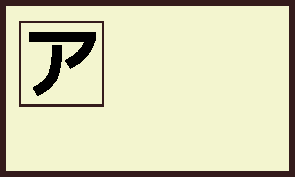
\includegraphics[scale=1.5]{../share/i/fcak.pdf}% Katakana
}{}
\\
\end{tabular}
\end{center}

        \caption{Flashcard type 1 (rōmaji - kana) }
        \label{fig:FlashCardTypeOne}
\end{figure}

\normalsize

Or to learn both:

\begin{figure}[H]
        \begin{center}
\begin{tabular}{cc}
\textbf{Front site rōmaji}&\textbf{Back site both}\\
\includegraphics[scale=1.5]{../share/i/fcar.pdf}% Rōmaji
&
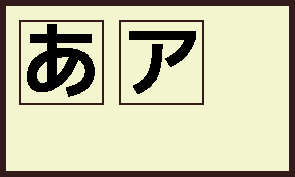
\includegraphics[scale=1.5]{../share/i/fcahk.pdf}% Hiragana/ Katakana
\\
\end{tabular}
\end{center}

        \caption{Flashcard type 2 (rōmaji - 2 kana)}
        \label{fig:FlashCardTypeTwo}
\end{figure}

\normalsize

To dive deep into Japanese of course skipping rōmaji is the preferred method:

\begin{figure}[H]
        \begin{center}
\begin{tabular}{cc}
\textbf{Front site Katakana}&\textbf{Back site Hiragana}\\
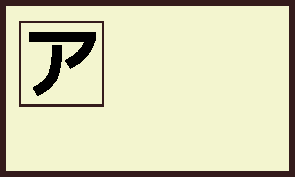
\includegraphics[scale=1.5]{../share/i/fcak.pdf}% Katakana
&
\includegraphics[scale=1.5]{../share/i/fcah.pdf}% Hiragana
\\
\end{tabular}
\end{center}

        \caption{Flashcard type 3 (katakana - hiragana)}
        \label{fig:FlashCardTypeThree}
\end{figure}

This training chapter can be used as an additional aid to learn
\textbf{\jtopic}. And also here it is important to develop ones own method.
However some hints on learning with this training chapter can be given.

\begin{description}

\item[Reading Loud:] While writing a \textbf{\jtopic} character in this book
        (and probably also later), read out loud the sound of the character.
        Always.

\item[Invent your own cribs:] One can (maybe should?) invent one crib per
        character by oneself. Especially if the characters is difficult to
        remember. It might be useful to write it down on the self created
        flashcard for that specific character.

\item[Regular Repetition:] It is of course possible to fill out all fields for
        one character in a very short time. The learning effect should be
        minimal though. Better is to fill out one row and then the second row
        an hour later, the third row the next day and so own. Oneself has to
        decide the rhythm of the repetition.

\item[Transcription:]  Search for a  \textbf{\jtopic} text and read it. Write
        for every \jtopic word the Roman letters. If this is possible without
        looking up the \jtopic, then the transcription should be reversed. Find
        some Japanese text written in Rōmaji and transcribe them to \jtopic on
        a different piece of paper.

\end{description}

\newpage

                                             % Katakana Hiragana
%----------------------------------------------------------------------------
\section{Katakana \jtl{a} Row}\jsec{片仮名ア行}\label{sec:KatakanaARow}

\Krow{arow}{a}{i}{u}{e}{o}

\label{letter:a}\KLETTER{a} The \jkatakana{} \jquotesingleja{ア} derives from
the \hyperref[sec:Radical]{radical} of the
\hyperref[sec:PhoneticCharacter]{phonetic character} \jquotesingleja{阿}.
Together with the \jkatakana{} \jquotesingleja{フ} \jtl{fu} the smaller sized
\jquotesingleja{ァ} gives the combination \jquotesingleja{ファ} and is
pronounced as such \jtl{fa}.

\label{letter:i}\KLETTER{i} The \jkatakana{} \jquotesingleja{イ} derives from
the \hyperref[sec:PhoneticCharacter]{phonetic characters} \jquotesingleja{伊}
left element (\hyperref[sec:Radical]{radical}). A smaller version
\jquotesingleja{ィ} is used in combinations with other letters and represents a
\hyperref[sec:Diphthong]{diphthong}.

\label{letter:u}\KLETTER{u} The \jkatakana{} \jquotesingleja{ウ} derives from
the \hyperref[sec:PhoneticCharacter]{phonetic character} \jquotesingleja{宇}. A
smaller version \jquotesingleja{ゥ} is used in combinations with other letters
and represents a \hyperref[sec:Diphthong]{diphthong} and is written as "w".
Even though the combination \jquotesingleja{トゥ} \jtl{tu} exist, it is
relatively new and many words do not use it. In this cases \jquotesingleja{ツ}
\jtl{tsu} is used. \jquotesingleja{ウ} can take \hyperref[sec:Dakuten]{dakuten}
to form \jquotesingleja{ヴ} \jtl{vu}, which is relatively new and can replace
\jquotesingleja{ブ} \jtl{bu}.

% UFuWaSimilarity
\subsection{\jtl{u}, \jtl{fu} and \jtl{wa} Similarity} \label{subsec:UFuWaSimilarity}

The Katakana characters \jquotesingleja{ウ}, \jquotesingleja{フ} and
\jquotesingleja{ワ} can be easily distinguished. All three have a different
stroke count. However the shape is similar. Therefore they can be mistaken.
Especially when they have no context.

\bigskip

\begin{figure}[H]
\begin{center}
\begin{tabular}{|c|c|c|}\hline
\KLETTER{u}&\KLETTER{fu}&\KLETTER{wa}\\\hline
\end{tabular}
\end{center}
\caption{\jtl{u}, \jtl{fu} and \jtl{wa} similarity}
\label{fig:UuFuAndWaSimilarity}
\end{figure}




\newpage

\label{letter:e}\KLETTER{e} The \jkatakana{} \jquotesingleja{エ} derives from
the \hyperref[sec:PhoneticCharacter]{phonetic characters} \jquotesingleja{江}
right element (\hyperref[sec:Radical]{radical}). A smaller version
\jquotesingleja{ェ} is used in combinations with other letters and express
\hyperref[sec:Mora]{morae} of foreign origin. For example \jquotesingleja{ヴェ}
is pronounced \jtl{ve}.

\label{letter:o}\KLETTER{o} The \jkatakana{} \jquotesingleja{オ} derives from
the \hyperref[sec:PhoneticCharacter]{phonetic character} \jquotesingleja{於}. A
smaller version \jquotesingleja{ォ} is used in combinations with other letters
and express' \hyperref[sec:Mora]{morae} of foreign origin. For example
\jquotesingleja{フォ } is pronounced \jtl{fo}.

\newpage

% ---------------------------------------------------------------------------
\subsection{\jtl{a}}\jsubsec{\jquotesingleja{ア}} \label{sec:KatakanaA}

\KatakanaHeader{a}{ The Katakana \jquotesingleja{ア} is written with two
        strokes. The first stroke starts horizontal. The second stroke is a
        curve with can be attached to the first stroke in hand writing, but not
        at the horizontal part - at the end of the first line.}
        \KatakanaTraining{a}

% ---------------------------------------------------------------------------
\subsection{\jtl{i}}\jsubsec{\jquotesingleja{イ}} \label{sec:KatakanaI}

\KatakanaHeader{i}{ The Katakana \jquotesingleja{イ} is written with one
stroke. The first stroke is a curve from upper right to lower left. The second
stroke is a vertical line attached to the first at the top.}
\KatakanaTraining{i}

% ---------------------------------------------------------------------------
\subsection{\jtl{u}}\jsubsec{\jquotesingleja{ウ}} \label{sec:KatakanaU}

\KatakanaHeader{u}{The Katakana \jquotesingleja{ウ} is written with three
strokes. The first stroke a small vertical line. The second a small vertical
line again and the third line a horizontal line connection the two others.}
\KatakanaTraining{u}

% ---------------------------------------------------------------------------
\subsection{\jtl{e}}\jsubsec{\jquotesingleja{エ}} \label{sec:KatakanaE}

\KatakanaHeader{e}{The Katakana \jquotesingleja{エ} is written with three
strokes. It is very geometrically consisting only out of horizontal and
vertical lines connected together.} \KatakanaTraining{e}

% ---------------------------------------------------------------------------
\subsection{\jtl{o}}\jsubsec{\jquotesingleja{オ}} \label{sec:KatakanaO}

\KatakanaHeader{o}{The Katakana \jquotesingleja{オ} is written with three
strokes. The first line is horizontal and together with the second stroke it
constructs a perfect crossing. The third stroke beginning lies at the center of
the crossing.} \KatakanaTraining{o}

% ---------------------------------------------------------------------------
\subsection{\jtl{a} Row Training}\jsubsec{片仮名ア行練習}
\Padding
\begin{longtable}[c]{p{2cm}p{2cm}p{3cm}p{6cm}p{2cm}}
\textit{Katakana}&\textit{Rōmaji}&\textit{Original}&\textit{Remark}&Origin\\\hline
ウエア&wuea&ware&          &English\\
エア  &ea  &air &          &English\\
エイ  &ei  &A   &the letter&English\\
\end{longtable}

\KanaSimpleTraining{Katakana to Rōmaji}{
\Transcribe{1.}{ウエア}{}{wear, ware}
\Transcribe{2.}{エア}{}{air}
\Transcribe{3.}{エイ}{}{A (the letter)}
\Transcribe{4.}{アイ}{}{I (the letter)}
\Transcribe{5.}{オウ}{}{O (the letter)}
%\Transcribe{6.}{イア}{}{ear}
}

\KanaSimpleTraining{Rōmaji to Katakana}{
\Transcribe{1.}{ea}{}{air}
\Transcribe{2.}{ai}{}{I (the letter)}
\Transcribe{3.}{ou}{}{O (the letter)}
\Transcribe{4.}{ei}{}{A (the letter)}
\Transcribe{5.}{uea}{}{wear, ware}
%\Transcribe{6.}{ia}{}{ear}
}

\newpage
\Padding
\begin{longtable}[c]{p{2cm}p{2cm}p{3cm}p{6cm}p{2cm}}
\textit{Katakana}&\textit{Rōmaji}&\textit{Original}&\textit{Remark}&Origin\\\hline
アイ  &ai  &I   &the letter&English\\
オウ  &ou  &O   &the letter&English\\
イア  &ia  &ear &          &English\\
\end{longtable}

\KanaSimpleTraining{English to Rōmaji}{
\Transcribe{1.}{ear}{}{}
\Transcribe{2.}{I (the letter)}{}{}
\Transcribe{3.}{air}{}{}
\Transcribe{4.}{O (the letter)}{}{}
\Transcribe{5.}{wear, ware}{}{}
%\Transcribe{6.}{A (the letter)}{}{}
}

\KanaSimpleTraining{English to Katakana}{
\Transcribe{1.}{I (the letter)}{}{}
\Transcribe{2.}{O (the letter)}{}{}
\Transcribe{3.}{air}{}{}
\Transcribe{4.}{ear}{}{}
\Transcribe{5.}{wear, ware}{}{}
%\Transcribe{6.}{A (the letter)}{}{}
}
\newpage
   % OK       OK
% ---------------------------------------------------------------------------
\section{Katakana \jtl{ka} Row}\jsec{片仮名カ行}\label{sec:KatakanaKaRow}

\Krow{karow}{ka}{ki}{ku}{ke}{ko}

\label{letter:ka}\KLETTER{ka} The  \textbf{katakana} \jquotesingleja{カ} is
pronounced \jtl{ka} and  derives from the
\hyperref[sec:PhoneticCharacter]{phonetic character}s \jquotesingleja{加} left
\hyperref[sec:Radical]{radical}.  A \hyperref[sec:Dakuten]{dakuten} version
exists and pronounced as \jtl{ga}.

%\hyperref[sec:Handakuten]{handakuten} does not exist in daily Japanese.
% \jquotesingleja{一ヵ所} {【いちかしょ】} (one place)
% \jquotesingleja{一ヶ所} {【いちかしょ】} (one place).
% 十ヵ条(十ヶ条)

\Note{Note}{

A smaller version \jquotesingleja{ヵ} is rare but used in combinations with
number particles.  For example in \jquotesingleja{一ヵ月} {【いっかげつ】} (one
month) and others.  This cases can also be written \jquotesingleja{一ヶ月}
{【いっかげつ】} (one month). Please see also \nameref{sec:KatakanaKe}. \Link
\href{https://ja.wikipedia.org/wiki/\%E3\%83\%B5}{ヵ}

}

\label{letter:ki}\KLETTER{ki} The \textbf{katakana} \jquotesingleja{キ} derives
from the \hyperref[sec:PhoneticCharacter]{phonetic character}s middle part of
either \jquotesingleja{機} or \jquotesingleja{幾}.  It is pronounced as
\jtl{ki}.  A \hyperref[sec:Dakuten]{dakuten} version exists and pronounced as
\jtl{gi}.


\label{letter:ku}\KLETTER{ku} The \textbf{katakana} \jquotesingleja{ク} derives
from the \hyperref[sec:PhoneticCharacter]{phonetic character}s left upper part
of \jquotesingleja{久}.  It is pronounced as \jtl{ku}.  A
\hyperref[sec:Dakuten]{dakuten} version exists and pronounced as \jtl{gu}.  A
smaller version exists, but is used for the Ainu Language.

\label{letter:ke}\KLETTER{ke} The \textbf{katakana} \jquotesingleja{ケ} derives
from the \hyperref[sec:PhoneticCharacter]{phonetic character}s upper and left
part of \jquotesingleja{介}.  It is pronounced as \jtl{ke}.  A
\hyperref[sec:Dakuten]{dakuten} version exists and pronounced as \jtl{ge}.  The
smaller version \jquotesingleja{ヶ} is explained in the following note.

\newpage

\Note{Note}{

A smaller version \jquotesingleja{ヶ} is rare but used in combinations with
number particles.  For example in \jquotesingleja{一ヶ月} {【いっかげつ】} (one
month) and others.  This cases can also be written \jquotesingleja{一ヵ月}
{【いっかげつ】} (one month). There are cases where only \jquotesingleja{ヶ}
can be written {七ヶ宿} {【シチカシュク】} (Place at the south west border of
the prefecture Miyagi).  In other rare cases this character can be pronounced
different \jquotesingleja{関ヶ原} {【せきがはら】} (Place at the south border
of the Gifu prefecture, known by the battle at 1600.). Please see also
\nameref{sec:KatakanaKa}. \Link
\href{https://ja.wikipedia.org/wiki/\%E3\%83\%B5}{ヵ}

}

\label{letter:ko}\KLETTER{ko} The \textbf{katakana} \jquotesingleja{コ} derives
from the \hyperref[sec:PhoneticCharacter]{phonetic character}s upper part of
\jquotesingleja{己}.  It is pronounced as \jtl{ko}.  A
\hyperref[sec:Dakuten]{dakuten} version exists and pronounced as \jtl{go}.



\newpage

% ---------------------------------------------------------------------------
\subsection{\jtl{ka}}\jsubsec{\jquotesingleja{カ}} \label{sec:KatakanaKa}

\KatakanaHeader{ka}{ \jtl{ka} is written with 2 strokes. Basically the same way
as the Hiragana \jquotesingleja{か} it looks like a squarish version, but
without the last stroke. The hook at the second stroke is less significant or
important.  } \KatakanaTraining{ka}

% ---------------------------------------------------------------------------
\subsection{\jtl{ki}}\jsubsec{\jquotesingleja{キ}} \label{sec:KatakanaKi}

\KatakanaHeader{ki}{ The shape alignment of the \jquotesingleja{キ} character
is not straight towards its environment. However the junctions are more or less
90 degrees.  } \KatakanaTraining{ki}

% ---------------------------------------------------------------------------
\subsection{\jtl{ku}}\jsubsec{\jquotesingleja{ク}} \label{sec:KatakanaKu}
% ---------------------------------------------------------------------------

\KatakanaHeader{ku}{ The first stroke is similar the stroke of
\jquotesingleja{ケ} is a curve. While the second stroke start aligned and
straight. } \KatakanaTraining{ku}

% ---------------------------------------------------------------------------
\subsection{\jtl{ke}}\jsubsec{\jquotesingleja{ケ}} \label{sec:KatakanaKe}

\KatakanaHeader{ke}{ The \jquotesingleja{ケ} is written with 3 strokes and the
first stroke is similar to the \jquotesingleja{ク}. The second stroke is
aligned and straight.  While the last stroke is a curve.  }
\KatakanaTraining{ke}

% ---------------------------------------------------------------------------
\subsection{\jtl{ko}}\jsubsec{\jquotesingleja{コ}} \label{sec:KatakanaKo}

\KatakanaHeader{ko}{ This character is almost a geometric figure composed out
of two strokes. However unless in European languages this are only 2 strokes
and not 3. The first stroke is the longest one and done similar with all
{漢字}. } \KatakanaTraining{ko}

% ---------------------------------------------------------------------------
\subsection{\jtl{ka} Row Training}\jsubsec{片仮名カ行練習}

\Padding
\begin{longtable}[c]{p{2cm}p{1.5cm}p{1.5cm}p{3cm}p{7cm}}
\textit{Katakana}&\textit{Rōmaji}&\textit{Original}&\textit{Remark}&Origin\\\hline
カキ  &kaki &kaki &柿 persimon&Japanese\\
ケア  &kea  &care &          &English\\
ケイ  &kei  &K    &the letter&English\\
\end{longtable}

\KanaSimpleTraining{Katakana to Rōmaji}{
\Transcribe{1.}{カキ}{}{persimmon}
\Transcribe{2.}{ココア}{}{cocoa}
\Transcribe{3.}{ケア}{}{care}
\Transcribe{4.}{コア}{}{core}
\Transcribe{5.}{ケーキ}{}{cake}
%\Transcribe{6.}{ケイ}{}{K (the letter)}
}

\KanaSimpleTraining{Rōmaji to Katakana}{
\Transcribe{1.}{kokoa}{}{cocoa}
\Transcribe{2.}{k$\overline{\mbox{e}}$ki}{}{cake}
\Transcribe{3.}{kea}{}{care}
\Transcribe{4.}{koa}{}{core}
\Transcribe{5.}{kaki}{}{persimmon}
%\Transcribe{6.}{kei}{}{K (the letter)}
}

\newpage

\Padding
%\begin{longtable}[c]{p{2cm}p{2cm}p{3cm}p{6cm}p{2cm}}
\begin{longtable}[c]{p{2cm}p{2.0cm}p{3.5cm}p{4cm}p{2.5cm}}
\textit{Katakana}&\textit{Rōmaji}&\textit{Original}&\textit{Remark}&Origin\\\hline
コア  &koa  &core &          &English\\
ココア&kokoa&cocoa& hot chocolate &English, from metathesis of Spanish cacao, from Nahuatl cacahuatl\\
ケーキ&kēki &cake &          &English\\
\end{longtable}


\KanaSimpleTraining{English to Rōmaji}{
\Transcribe{1.}{persimon}{}{}
\Transcribe{2.}{cocoa}{}{}
\Transcribe{3.}{care}{}{}
\Transcribe{4.}{core}{}{}
\Transcribe{5.}{K (the letter)}{}{}
%\Transcribe{6.}{cake}{}{}
}

\KanaSimpleTraining{English to Katakana}{
\Transcribe{1.}{cocoa}{}{}
\Transcribe{2.}{cake}{}{}
\Transcribe{3.}{care}{}{}
\Transcribe{4.}{persimon}{}{}
\Transcribe{5.}{K (the letter)}{}{}
%\Transcribe{6.}{core}{}{}
}

\newpage
  % OK
%----------------------------------------------------------------------------
\section{Katakana \jtl{sa} Row}\jsec{片仮名サ行}\label{sec:KatakanaSaRow}

\Krow{sarow}{sa}{shi}{su}{se}{so}

\label{letter:sa}\KLETTER{sa} The  \textbf{katakana} \jquotesingleja{サ} is
pronounced \jtl{sa} and derives from the
\hyperref[sec:PhoneticCharacter]{phonetic character}s \jquotesingleja{散} upper
left corner \hyperref[sec:Radical]{radical}.  A \hyperref[sec:Dakuten]{dakuten}
version exists and pronounced as \jtl{za}.

\label{letter:shi}\KLETTER{shi} The \textbf{katakana} \jquotesingleja{シ}
derives from the \hyperref[sec:PhoneticCharacter]{phonetic character} 
\jquotesingleja{之 }.  It is pronounced as \jtl{shi}.  A
\hyperref[sec:Dakuten]{dakuten} version exists and pronounced as \jtl{ji}.

\Note{Note}{Please see section \nameref{subsec:ShiTsuAmbiguity} for the
explanation how to write and distinguish \jtl{shi} and \jtl{tsu}.  }

\label{letter:su}\KLETTER{su} The \textbf{katakana} \jquotesingleja{ス} derives
from the \hyperref[sec:PhoneticCharacter]{phonetic character}s right lower part
of \jquotesingleja{須}.  It is pronounced as \jtl{su}.  A
\hyperref[sec:Dakuten]{dakuten} version exists and pronounced as \jtl{zu}.

\label{letter:se}\KLETTER{se} The \textbf{katakana} \jquotesingleja{セ} derives
from the \hyperref[sec:PhoneticCharacter]{phonetic character}s middle left part
of \jquotesingleja{世}.  It is pronounced as \jtl{se}.  A
\hyperref[sec:Dakuten]{dakuten} version exists and pronounced as \jtl{ze}.

\newpage

\label{letter:so}\KLETTER{so} The \textbf{katakana} \jquotesingleja{ソ} derives
from the \hyperref[sec:PhoneticCharacter]{phonetic character}s upper right part
of \jquotesingleja{曽}.  It is pronounced as \jtl{so}.  A
\hyperref[sec:Dakuten]{dakuten} version exists and pronounced as \jtl{zo}.

% SoRiNAmbiguity
\subsection{\jtl{so}, \jtl{ri} and \jtl{n} Ambiguity} \label{subsec:SoRiNAmbiguity}

The Katakana characters \jquotesingleja{ソ}, \jquotesingleja{リ} and
\jquotesingleja{ン} can be difficult to distinguish. All three are made out of
only 2 strokes. And especially \jtl{so} and \jtl{n} can be hard to tell. In a
sentence of course the context can help a lot.  But what are the rules for this
characters to write properly and distinguish?

\bigskip

\begin{figure}[H]
\begin{center}
\begin{tabular}{|c|c|c|}\hline
\KLETTER{so}&\KLETTER{n}&\KLETTER{ri}\\\hline
\end{tabular}
\end{center}
\caption{\jtl{so}, \jtl{ri} and \jtl{n} ambiguity}
\label{fig:SoRiAndNAmbiguity}
\end{figure}

\CharacterExplanation{soexplanation}{

To write the letter \jtl{so} it is important to align both lines
\textbf{horizontally} (red line) and to \textbf{non-align} the ends (blue line)
vertically. In this way it is possible to distinguish \jtl{so} from \jtl{n},
but not from \jtl{ri}. To also distinguish it from \jtl{ri} you have to write
the first stroke not horizontally nor vertically (green line).

}

\CharacterExplanation{nexplanation}{

To write the letter \jtl{n} it is important to a align both lines
\textbf{vertically} (red line) and to \textbf{non-align} the ends (blue line).
In this way it is possible to distinguish \jtl{n} from \jtl{so}. If both lines
are aligned there should not be a problem to distinguish it from \jtl{ri}.
Usually the angle of the green line is different, but only a small indicator.

}

\CharacterExplanation{riexplanation}{

To write the letter \jtl{ri} it is important to \textbf{align} both of the line
beginnings \textbf{horizontally} (red line) and to make sure that both lines
are \textbf{parallel} (green lines). There should be \textbf{no alignment} on
the left side (blue line) \textbf{vertically}. The difference between \jtl{so}
and \jtl{ri} is that \jtl{ri} need to start with two \textbf{parallel} lines
wile \jtl{so} should not. Please compare the left green line for an
explanation.

}



\newpage
% ---------------------------------------------------------------------------
\subsection{\jtl{sa}}\jsubsec{\jquotesingleja{サ}}\label{sec:KatakanaSa}

\KatakanaHeader{sa}{ Katakana \jquotesingleja{サ} is written with three
strokes. All crossings of strokes are in a 90 degree angle.  The starts of all
strokes are aligned either horizontally or vertically. The last stroke has a
curve.} \KatakanaTraining{sa}

% ---------------------------------------------------------------------------
\subsection{\jtl{shi}}\jsubsec{\jquotesingleja{シ}}\label{sec:KatakanaShi}

\KatakanaHeader{shi}{ The Katakana \jquotesingleja{シ} is written with three
strokes. All three strokes are aligned vertically in the beginning. Please see
section \nameref{subsec:ShiTsuAmbiguity}.} \KatakanaTraining{shi}

% ---------------------------------------------------------------------------
\subsection{\jtl{su}}\jsubsec{\jquotesingleja{ス}}\label{sec:KatakanaSu}

\KatakanaHeader{su}{The Katakana \jquotesingleja{ス} is written with two
strokes. The first stroke starts horizontally aligned. The second stroke
touches the first stroke at the beginning.} \KatakanaTraining{su}

% ---------------------------------------------------------------------------
\subsection{\jtl{se}}\jsubsec{\jquotesingleja{セ}}\label{sec:KatakanaSe}

\KatakanaHeader{se}{ The Katakana \jquotesingleja{セ} is written with two
strokes. The crossing has \textbf{no} 90 degree angle. The curve of the second
stroke as almost a 90 degree angle. } \KatakanaTraining{se}

% ---------------------------------------------------------------------------
\subsection{\jtl{so}}\jsubsec{\jquotesingleja{ソ}}\label{sec:KatakanaSo}

\KatakanaHeader{so}{ The Katakana \jquotesingleja{ソ} is written with two
strokes. The first stroke is not aligned vertically but it is aligned
horizontally withe the second stroke. Please see section
\nameref{subsec:SoRiNAmbiguity}.} \KatakanaTraining{so}

% ---------------------------------------------------------------------------
\subsection{\jtl{sa} Row Training}\jsubsec{片仮名サ行練習}\label{sec:SaRowTraining}
% 3 78 エキス
%3 357 スカイ
%3 360 スキー
%3 3 アイス
%3 111 ガーゼ
%3 146 イエス
\Padding
\begin{longtable}[c]{p{2cm}p{2cm}p{3cm}p{6cm}p{2cm}}
\textit{Katakana}&\textit{Rōmaji}&\textit{Original}&\textit{Remark}&\textit{Origin}\\\hline
エキス&ekisu&ex(tract)&extract&Dutch\\
スカイ&sukai&sky&&English\\
スキー&sukī&ski&noun for skiing&English\\
\end{longtable}
\KanaSimpleTraining{Katakana to Rōmaji}{
\Transcribe{1.}{エキス}{}{extract}      % ekisu
\Transcribe{2.}{スカイ}{}{sky}          % sukai
\Transcribe{3.}{スキー}{}{ski}          % sukī
\Transcribe{4.}{アイス}{}{ice}          % aisu
\Transcribe{5.}{ガーゼ}{}{gauze}        % gāze
%\Transcribe{6.}{イエス}{}{Jesus}        % iesu
}

\KanaSimpleTraining{Rōmaji to Katakana}{
\Transcribe{1.}{sukai}{}{sky}         % sukai
\Transcribe{2.}{ekisu}{}{extract}     % ekisu
\Transcribe{3.}{aisu}{}{ice}          % aisu
\Transcribe{4.}{suki}{}{ski}          % sukī
\Transcribe{5.}{iesu}{}{Jesus}        % iesu
%\Transcribe{6.}{gāze}{}{gauze}        % gāze
}

\newpage

\Padding
\begin{longtable}[c]{p{2cm}p{2cm}p{3cm}p{6cm}p{2cm}}
\textit{Katakana}&\textit{Rōmaji}&\textit{Original}&\textit{Remark}&Origin\\\hline
アイス&aisu&ice&water ice, ice cream&English\\
ガーゼ&gāze&Gaze&gauze&German\\
イエス&iesu&Jesus&Jesus&Portuguese\\
\end{longtable}
\KanaSimpleTraining{English to Rōmaji}{
\Transcribe{1.}{extract}{}{}       % ekisu
\Transcribe{2.}{sky}{}{}           % sukai
\Transcribe{3.}{Jesus}{}{}         % iesu
\Transcribe{4.}{gauze}{}{}         % gāze
\Transcribe{5.}{ice}{}{}           % aisu
%\Transcribe{6.}{ski}{}{}           % sukī
}

\KanaSimpleTraining{English to Katakana}{
\Transcribe{1.}{sky}{}{}           % sukai
\Transcribe{2.}{gauze}{}{}         % gāze
\Transcribe{3.}{ice}{}{}           % aisu
\Transcribe{4.}{Jesus}{}{}         % iesu
\Transcribe{5.}{extract}{}{}       % ekisu
%\Transcribe{6.}{ski}{}{}           % sukī
}

\newpage
  % OK
% ---------------------------------------------------------------------------
\section{Katakana \jtl{ta} Row}\jsec{片仮名タ行}\label{sec:KatakanaTaRow}

\Krow{tarow}{ta}{chi}{tsu}{te}{to}

\label{letter:ta}\KLETTER{ta} The  \textbf{katakana} \jquotesingleja{タ} is
pronounced \jtl{ta} and derives from the
\hyperref[sec:PhoneticCharacter]{phonetic character}s \jquotesingleja{多 }
upper or lover \hyperref[sec:Radical]{radical}.  A
\hyperref[sec:Dakuten]{dakuten} version exists and pronounced as \jtl{da}.

\label{letter:chi}\KLETTER{chi} The \textbf{katakana} \jquotesingleja{チ}
derives from the \hyperref[sec:PhoneticCharacter]{phonetic character} 
\jquotesingleja{千}.  It is pronounced as \jtl{chi}.  A
\hyperref[sec:Dakuten]{dakuten} version exists and pronounced as \jtl{ji}.

\label{letter:tsu}\KLETTER{tsu} The \textbf{katakana} \jquotesingleja{ツ}
derives from the \hyperref[sec:PhoneticCharacter]{phonetic character}s
\jquotesingleja{州} or \jquotesingleja{川} .  It is pronounced as \jtl{tsu}.  A
\hyperref[sec:Dakuten]{dakuten} version exists and pronounced as \jtl{zu}.

\label{letter:te}\KLETTER{te} The \textbf{katakana} \jquotesingleja{テ} derives
from the \hyperref[sec:PhoneticCharacter]{phonetic character}s lower left part
of \jquotesingleja{天 }.  It is pronounced as \jtl{te}.  A
\hyperref[sec:Dakuten]{dakuten} version exists and pronounced as \jtl{de}.

\newpage

\label{letter:to}\KLETTER{to} The \textbf{katakana} \jquotesingleja{ト} derives
from the \hyperref[sec:PhoneticCharacter]{phonetic character}s right part of
\jquotesingleja{止}.  It is pronounced as \jtl{to}.  A
\hyperref[sec:Dakuten]{dakuten} version exists and pronounced as \jtl{do}.

% ShiTsuAmbiguity
\subsection{\jtl{shi} and \jtl{tsu} Ambiguity} \label{subsec:ShiTsuAmbiguity}

% シ
% ツ

The Katakana characters \jquotesingleja{シ} and \jquotesingleja{ツ} are
difficult to distinguish.  Both are made out of 3 strokes and even the length
are equal. In a sentence of course the context can help a lot. But what are the
rules for this characters to write properly and distinguish?

\bigskip

\begin{figure}[H]
\begin{center}
\begin{tabular}{|c|c|}\hline
\KLETTER{shi}&\KLETTER{tsu}\\\hline
\end{tabular}
\end{center}
\caption{\jtl{shi} and \jtl{tsu} ambiguity}
\label{fig:ShiAndTsuAmbiguity}
\end{figure}

\CharacterExplanation{shiexplanation}{

To write the letter \jtl{shi} it is important to align three lines
\textbf{vertically} (red line) and to \textbf{non-align} the ends (blue line).
In this way it is possible to distinguish \jtl{shi} from \jtl{tsu}. Of course
also the angle of the frist two lines are different, but in hadwriting this is
difficult to match. As a rule of thumb make the third line double as long as
the first two but short enough to not align it at the end.

}

\CharacterExplanation{tsuexplanation}{

To write the letter \jtl{tsu} it is important to align all tree lines
\textbf{horizontally} (red line) and to \textbf{non-align} the ends (blue
line). In this way it is possible to distinguish \jtl{tsu} from \jtl{shi}. Of
course also the angle of the first two lines are different, but in handwriting
this is difficult to match. As a rule of thumb make the third line double as
long as the first two but short enough to not align it at the end.

}



\newpage

% ---------------------------------------------------------------------------
\subsection{\jtl{ta}}\jsubsec{\jquotesingleja{タ}}\label{sec:KatakanaTa}

\KatakanaHeader{ta}{ Katakana \jtl{ta} is written with three strokes. The first
stroke is a small curve. The secosnd stroke starts horizontally attached to the
first stroke. The third stroke ends at the second stroke.}
\KatakanaTraining{ta}

% ---------------------------------------------------------------------------
\subsection{\jtl{chi}}\jsubsec{\jquotesingleja{チ}}\label{sec:KatakanaChi}

\KatakanaHeader{chi}{ Katakana \jtl{chi} is written with three strokes. The
first stroke is a light curve. The second ihorizontally straight line. The
third line is a curve that joints the first and the second.}
\KatakanaTraining{chi}

% ---------------------------------------------------------------------------
\subsection{\jtl{tsu}}\jsubsec{\jquotesingleja{ツ}}\label{sec:KatakanaTsu}

\KatakanaHeader{tsu}{Katakana \jtl{tsu} is written with three strokes. The
first and second stroke are short. And the beginning of all three strokes is
aligned horizontally. The third stroke is the longest, but the end is not
alignd wit the beginning of the first stroke. } \KatakanaTraining{tsu}

% ---------------------------------------------------------------------------
\subsection{\jtl{te}}\jsubsec{\jquotesingleja{テ}}\label{sec:KatakanaTe}

\KatakanaHeader{te}{ Katakana \jtl{te} is written with three strokes. The first
stroke is the shortest and horizontally. The second stroke is not aligned
vertically in the beginning, but also perfectly horizontally. The third stroke
is a small curve attached to the middle of the second stroke. }
\KatakanaTraining{te}

% ---------------------------------------------------------------------------
\subsection{\jtl{to}}\jsubsec{\jquotesingleja{ト}}\label{sec:KatakanaTo}

\KatakanaHeader{to}{ Katakana \jtl{to} is written with 2 strokes. The first
stroke is a vertical line. Attached to this line there is short straight line
to the right. In some hand writings this line is a small curve to the right.}
\KatakanaTraining{to}

% ---------------------------------------------------------------------------
\subsection{\jtl{ta} Row Training}\jsubsec{片仮名タ行練習}
\Padding
\begin{longtable}[c]{p{2cm}p{2cm}p{3cm}p{6cm}p{2cm}}
\textit{Katakana}&\textit{Rōmaji}&\textit{Original}&\textit{Remark}&\textit{Origin}\\\hline
エステ        &esutei    &esthé(tique)&beauty salon, esthetic clinic    &French\\
サイト        &saito     &site        &&English\\
タスク        &tasuku    &task        &&English\\
\end{longtable}

\KanaSimpleTraining{Katakana to Rōmaji}{
\Transcribe{1.}{エステ}{}{esthé(tique)}
\Transcribe{2.}{サイト}{}{site}
\Transcribe{3.}{タスク}{}{task}
\Transcribe{4.}{テスト}{}{test}
\Transcribe{5.}{スーツアクター}{}{suit actor}
%\Transcribe{6.}{テキスト}{}{text}
}

\KanaSimpleTraining{Rōmaji to Katakana}{
\Transcribe{1.}{saito}{}{site}
\Transcribe{2.}{tasuku}{}{task}
\Transcribe{3.}{esute}{}{esthé(tique)}
\Transcribe{4.}{sūtsuakutā}{}{suit actor}
\Transcribe{5.}{tesuto}{}{test}
%\Transcribe{6.}{テキスト}{}{text}
}

\newpage
\Padding
\begin{longtable}[c]{p{2.6cm}p{2cm}p{1.8cm}p{6.6cm}p{1.8cm}}
\textit{Katakana}&\textit{Rōmaji}&\textit{Original}&\textit{Remark}&\textit{Origin}\\\hline
テスト        &tesuto    &test        &                                 &English\\
スーツアクター&sūtsuakutā&suit actor  &wearing cartoon-character costume&English\\
テキスト      &tekisuto  &text        &                                 &English\\
\end{longtable}

\KanaSimpleTraining{English to Rōmaji}{
\Transcribe{1.}{task}{}{}
\Transcribe{2.}{esthé(tique)}{}{}
\Transcribe{3.}{text}{}{}
\Transcribe{4.}{test}{}{}
\Transcribe{5.}{suit actor}{}{}
%\Transcribe{6.}{site}{}{}
}

\KanaSimpleTraining{English to Katakana}{
\Transcribe{2.}{esthé(tique)}{}{}
\Transcribe{4.}{test}{}{}
\Transcribe{5.}{suit actor}{}{}
\Transcribe{3.}{text}{}{}
\Transcribe{6.}{site}{}{}
%\Transcribe{1.}{task}{}{}
}

\newpage
  % OK
% ---------------------------------------------------------------------------
\section{Katakana \jtl{na} Row}\jsec{片仮名ナ行}\label{sec:KatakanaNaRow}

\Krow{narow}{na}{ni}{nu}{ne}{no}

\label{letter:na}\KLETTER{na} The  \textbf{katakana} \jquotesingleja{ナ} is
pronounced \jtl{na} and  derives from the
\hyperref[sec:PhoneticCharacter]{phonetic character}s \jquotesingleja{奈} upper
left corner part.  A \hyperref[sec:Dakuten]{dakuten} version  or
\hyperref[sec:Handakuten]{handakuten} do not exist.

\label{letter:ni}\KLETTER{ni} The  \textbf{katakana} \jquotesingleja{ニ} is
pronounced \jtl{ni} and  derives from the
\hyperref[sec:PhoneticCharacter]{phonetic character}s \jquotesingleja{奈} upper
right part.  A \hyperref[sec:Dakuten]{dakuten} version  or
\hyperref[sec:Handakuten]{handakuten} do not exist.

\label{letter:nu}\KLETTER{nu} The  \textbf{katakana} \jquotesingleja{ヌ} is
pronounced \jtl{nu} and  derives from the
\hyperref[sec:PhoneticCharacter]{phonetic character}s \jquotesingleja{奴} right
part.  A \hyperref[sec:Dakuten]{dakuten} version  or
\hyperref[sec:Handakuten]{handakuten} do not exist.

\Note{Note}{%

The characters \hyperref[letter:no]{\jquotesingleja{ノ}},
\hyperref[letter:me]{\jquotesingleja{メ}} and
\hyperref[letter:nu]{\jquotesingleja{ヌ}} are similar and it is easy to make a
mistake. To distinguish \jquotesingleja{メ} it is important to make all strokes
long enough.

}%


\newpage

\label{letter:ne}\KLETTER{ne} The  \textbf{katakana} \jquotesingleja{ネ} is
pronounced \jtl{ne} and  derives from the
\hyperref[sec:PhoneticCharacter]{phonetic character}s \jquotesingleja{祢} upper
left  part.  A \hyperref[sec:Dakuten]{dakuten} version  or
\hyperref[sec:Handakuten]{handakuten} do not exist.

\label{letter:no}\KLETTER{no} The  \textbf{katakana} \jquotesingleja{ノ} is
pronounced \jtl{no} and  derives from the
\hyperref[sec:PhoneticCharacter]{phonetic character}s \jquotesingleja{乃} upper
left part.  A \hyperref[sec:Dakuten]{dakuten} version  or
\hyperref[sec:Handakuten]{handakuten} do not exist.

\Note{Note}{%

The characters \hyperref[letter:no]{\jquotesingleja{ノ}},
\hyperref[letter:me]{\jquotesingleja{メ}} and
\hyperref[letter:nu]{\jquotesingleja{ヌ}} are similar and it is easy to make a
mistake. To distinguish \jquotesingleja{メ} it is important to make all strokes
long enough.

}%

\newpage

% ---------------------------------------------------------------------------
\subsection{\jtl{na}}\jsubsec{\jquotesingleja{ナ}} \label{sec:KatakanaNa}

\KatakanaHeader{na}{ Katakana \jtl{na} is written with two strokes.} \KatakanaTraining{na}

% ---------------------------------------------------------------------------
\subsection{\jtl{ni}}\jsubsec{\jquotesingleja{ニ}} \label{sec:KatakanaNi}

\KatakanaHeader{ni}{ Katakana \jtl{ni} is written with two strokes.} \KatakanaTraining{ni}

% ---------------------------------------------------------------------------
\subsection{\jtl{nu}}\jsubsec{\jquotesingleja{ヌ}} \label{sec:KatakanaNu}

\KatakanaHeader{nu}{Katakana \jtl{nu} is written with two strokes.} \KatakanaTraining{nu}

% ---------------------------------------------------------------------------
\subsection{\jtl{ne}}\jsubsec{\jquotesingleja{ネ}} \label{sec:KatakanaNe}

\KatakanaHeader{ne}{Katakana \jtl{ne} is written with three strokes.} \KatakanaTraining{ne}

% ---------------------------------------------------------------------------
\subsection{\jtl{no}}\jsubsec{\jquotesingleja{ノ}} \label{sec:KatakanaNo}

\KatakanaHeader{no}{Katakana \jtl{no} is written with one stroke.} \KatakanaTraining{no}

% ---------------------------------------------------------------------------
\subsection{ \jtl{na} Row Training}\jsubsec{片仮名ナ行練習}
\Padding
\begin{longtable}[c]{p{2cm}p{2cm}p{3cm}p{6cm}p{2cm}}
\textit{Katakana}&\textit{Rōmaji}&\textit{Original}&\textit{Remark}&\textit{Origin}\\\hline
ナース  &nāsu &nurse      &                                        &English\\
ネット  &netto&net(work)  &                                        &English\\
アニス &anisu&anise      &pimpinella anisum                       &\\
\end{longtable}

\KanaSimpleTraining{Katakana to Rōmaji}{
\Transcribe{1.}{ネット}{}{net(work)}
\Transcribe{2.}{ナース}{}{nurse}
\Transcribe{3.}{アニス}{}{anise}
\Transcribe{4.}{ニート}{}{NEET}
\Transcribe{5.}{ナイター}{}{night + -er}
%\Transcribe{6.}{ノート}{}{note}
}

\KanaSimpleTraining{Rōmaji to Katakana}{
\Transcribe{1.}{nōto}{}{note}
\Transcribe{2.}{netto}{}{net(work)}
\Transcribe{3.}{anisu}{}{anise}
\Transcribe{4.}{nāsu}{}{nurse}
\Transcribe{5.}{naitā}{}{night + -er}
%\Transcribe{4.}{ニート}{}{NEET}
}

\newpage
\Padding
\begin{longtable}[c]{p{2cm}p{2cm}p{3cm}p{6cm}p{2cm}}
\textit{Katakana}&\textit{Rōmaji}&\textit{Original}&\textit{Remark}&\textit{Origin}\\\hline
ニート  &nīto &NEET       &Not in Education, Employment or Training&English\\
ナイター&naitā&night + -er&     a night game                       &English\\
ノート  &nōto &note       & note, notebook                         &English\\
\end{longtable}
\KanaSimpleTraining{English to Rōmaji}{
\Transcribe{1.}{anise}{}{}
\Transcribe{2.}{net(work)}{}{}
\Transcribe{3.}{note}{}{}
\Transcribe{4.}{nurse}{}{}
\Transcribe{5.}{NEET}{}{}
%\Transcribe{5.}{night + -er}{}{}
}

\KanaSimpleTraining{English to Katakana}{
\Transcribe{1.}{nurse}{}{}
\Transcribe{2.}{note}{}{}
\Transcribe{3.}{net(work)}{}{}
\Transcribe{4.}{anise}{}{}
\Transcribe{5.}{night + -er}{}{}
%\Transcribe{4.}{NEET}{}{}
}

\newpage
  %
% ---------------------------------------------------------------------------
\section{ Katakana \jtl{ha} Row}\jsec{片仮名ハ行}\label{sec:KatakanaHaRow}

\Krow{harow}{ha}{hi}{fu}{he}{ho}

\label{letter:ha}\KLETTER{ha} The \textbf{katakana} \jquotesingleja{ハ} is
pronounced \jtl{ha} and derives from the
\hyperref[sec:PhoneticCharacter]{phonetic character} \jquotesingleja{八 }.  A
\hyperref[sec:Dakuten]{dakuten} version exists and pronounced as \jtl{ba}.

\label{letter:hi}\KLETTER{hi} The \textbf{katakana} \jquotesingleja{ヒ} derives
from the \hyperref[sec:PhoneticCharacter]{phonetic characters}
\jquotesingleja{比} reight \hyperref{sec:Radical}{radical}. It is pronounced as
\jtl{hi}. A \hyperref[sec:Dakuten]{dakuten} version exists and pronounced as
\jtl{bi}.

\label{letter:fu}\KLETTER{fu} The \textbf{katakana} \jquotesingleja{フ} derives
from the \hyperref[sec:PhoneticCharacter]{phonetic characters} upper left part
of \jquotesingleja{不 }. It is pronounced as \jtl{fu}. A
\hyperref[sec:Dakuten]{dakuten} version exists and pronounced as \jtl{bu}.

\label{letter:he}\KLETTER{he} The \textbf{katakana} \jquotesingleja{ヘ} derives
from the \hyperref[sec:PhoneticCharacter]{phonetic characters} right
\hyperref{sec:Radical}{radical} of \jquotesingleja{部}. It is pronounced as
\jtl{he}. A \hyperref[sec:Dakuten]{dakuten} version exists and pronounced as
\jtl{be}.

\Warn{Warning}{The Katakana \jquotesingleja{ヘ} is the same character as the
        \hyperref[sec:Hiragana]{hiragana} \jquotesingleja{へ}. In some
        documents they can be distinguished because the font is different.
        However in genral they are the same. }

\label{letter:ho}\KLETTER{ho} The \textbf{katakana} \jquotesingleja{ホ} derives
from the \hyperref[sec:PhoneticCharacter]{phonetic characters} lower right part
of \jquotesingleja{保} which by itself is the \hyperref[sec:Radical]{radical}
and \hyperref[sec:Kanji]{kanji} of tree. It is pronounced as \jtl{ho}. A
\hyperref[sec:Dakuten]{dakuten} version exists and pronounced as \jtl{bo}.

% UFuWaSimilarity
\subsection{\jtl{u}, \jtl{fu} and \jtl{wa} Similarity} \label{subsec:UFuWaSimilarity}

The Katakana characters \jquotesingleja{ウ}, \jquotesingleja{フ} and
\jquotesingleja{ワ} can be easily distinguished. All three have a different
stroke count. However the shape is similar. Therefore they can be mistaken.
Especially when they have no context.

\bigskip

\begin{figure}[H]
\begin{center}
\begin{tabular}{|c|c|c|}\hline
\KLETTER{u}&\KLETTER{fu}&\KLETTER{wa}\\\hline
\end{tabular}
\end{center}
\caption{\jtl{u}, \jtl{fu} and \jtl{wa} similarity}
\label{fig:UuFuAndWaSimilarity}
\end{figure}




\newpage

% ハヒフヘホ
% ---------------------------------------------------------------------------
\subsection{\jtl{ha}}\jsubsec{\jquotesingleja{ハ}} \label{sec:KatakanaHa}

\KatakanaHeader{ha}{ The Katakana \jquotesingleja{ハ} is written with two
strokes. Non of them is straight.} \KatakanaTraining{ha}

% ---------------------------------------------------------------------------
\subsection{\jtl{hi}}\jsubsec{\jquotesingleja{ヒ}} \label{sec:KatakanaHi}

\KatakanaHeader{hi}{ The Katakana \jquotesingleja{ヒ} is written with two
strokes. One stroke from right to left. The other stroke from up to down and
then a curve.  The difficulty of this character is to hit the first stroke with
the second. } \KatakanaTraining{hi}

% ---------------------------------------------------------------------------
\subsection{\jtl{fu}}\jsubsec{\jquotesingleja{フ}} \label{sec:KatakanaFu}

\KatakanaHeader{fu}{The pronunciation of Katakana \jquotesingleja{フ} is
\textbf{not} \jtl{hu} it is \jtl{fu} and it is written with only one stroke. }
\KatakanaTraining{fu}

% ---------------------------------------------------------------------------
\subsection{\jtl{he}}\jsubsec{\jquotesingleja{ヘ}} \label{sec:KatakanaHe}

\KatakanaHeader{he}{Katakana \jquotesingleja{ヘ} is written with one stroke
from left to right. This is the same character as
\hyperref[sec:Hiragana]{hiragana} \jtl{he}.} \KatakanaTraining{he}

% ---------------------------------------------------------------------------
\subsection{\jtl{ho}}\jsubsec{\jquotesingleja{ホ}} \label{sec:KatakanaHo}

\KatakanaHeader{ho}{

The Katakana \jquotesingleja{ホ} character reminds at the Kanji for tree and is
also written in the same order and with the same amount of stroke. However the
left and right 'root' is not connected to the base. In cursive writing the
character is written with a hook-stroke as the second stroke. This is abstract
available even in the bold form where the second stroke has a small curve at
the end.

}
\KatakanaTraining{ho}

% ---------------------------------------------------------------------------
\subsection{\jtl{ha} Row Training}\jsubsec{片仮名ハ行練習}\label{sec:HaRowTraining}
\Padding
\begin{longtable}[c]{p{3cm}p{2cm}p{3cm}p{5cm}p{2cm}}
\textit{Katakana}&\textit{Rōmaji}&\textit{Original}&\textit{Remark}&\textit{Origin}\\\hline
ホットケーキ&hottokēki&hotcake    &a pancake                         &English\\
コーヒー    &kōhī     &koffie     &珈琲  coffee                      &Dutch\\
ソフト      &sofuto   &soft(ware) &                                  &English \\
\end{longtable}

\KanaSimpleTraining{Katakana to Rōmaji}{
\Transcribe{1.}{ホットケーキ}{}{hotcake}
\Transcribe{2.}{コーヒー}{}{coffee}
\Transcribe{3.}{ソフト}{}{soft(ware)}
\Transcribe{4.}{ハイタッチ}{}{high five}
\Transcribe{5.}{ハウス}{}{house}
%\Transcribe{6.}{ハイネック}{}{high neck}
}

\KanaSimpleTraining{Rōmaji to Katakana}{
\Transcribe{1.}{kōhī}{}{coffee}
\Transcribe{2.}{hottokēki}{}{hotcake}
\Transcribe{3.}{haitacchi}{}{high five}
\Transcribe{4.}{sofuto}{}{soft(ware)}
\Transcribe{5.}{hainekku}{}{high neck}
%\Transcribe{6.}{hausu}{}{house}
}

\newpage
\Padding
\begin{longtable}[c]{p{2cm}p{2cm}p{3cm}p{6cm}p{2cm}}
\textit{Katakana}&\textit{Rōmaji}&\textit{Original}&\textit{Remark}&\textit{Origin}\\\hline
ハイタッチ  &haitacchi&high touch &high five                         &English\\
ハウス      &hausu    &Haus, house&                                  &English, German\\
ハイネック  &hainekku &high neck  &turtle neck style sweater or shirt&English\\
\end{longtable}
\KanaSimpleTraining{English to Rōmaji}{
\Transcribe{1.}{coffee}{}{}
\Transcribe{2.}{hotcake}{}{}
\Transcribe{3.}{high five}{}{}
\Transcribe{4.}{software}{}{}
\Transcribe{5.}{high neck}{}{}
%\Transcribe{6.}{house}{}{}
}

\KanaSimpleTraining{English to Katakana}{
\Transcribe{1.}{hotcake}{}{}
\Transcribe{2.}{high five}{}{}
\Transcribe{3.}{coffee}{}{}
\Transcribe{4.}{high neck}{}{}
\Transcribe{5.}{house}{}{}
%\Transcribe{6.}{software}{}{}
}

\newpage
  % OK
% ---------------------------------------------------------------------------
\section{Katakana \jtl{ma} Row}\jsec{片仮名マ行}\label{sec:KatakanaMaRow}

\Krow{marow}{ma}{mi}{mu}{me}{mo}

\label{letter:ma}\KLETTER{ma} The  \textbf{katakana} \jquotesingleja{マ} is
pronounced \jtl{ma} and derives from the
\hyperref[sec:PhoneticCharacter]{phonetic character}s \jquotesingleja{末} upper
two parallel horizontal strokes.  A \hyperref[sec:Dakuten]{dakuten} or
\hyperref[sec:Handakuten]{handakuten} version do not exist.

\label{letter:mi}\KLETTER{mi} The  \textbf{katakana} \jquotesingleja{ミ} is
pronounced \jtl{mi} and derives from the
\hyperref[sec:PhoneticCharacter]{phonetic character} \jquotesingleja{三}.  A
\hyperref[sec:Dakuten]{dakuten} or \hyperref[sec:Handakuten]{handakuten}
version do not exist.

\label{letter:mu}\KLETTER{mu} The  \textbf{katakana} \jquotesingleja{ム} is
pronounced \jtl{mu} and derives from the
\hyperref[sec:PhoneticCharacter]{phonetic character}s \jquotesingleja{牟 }
upper part.  A \hyperref[sec:Dakuten]{dakuten} or
\hyperref[sec:Handakuten]{handakuten} version do not exist.

\newpage

\label{letter:me}\KLETTER{me} The  \textbf{katakana} \jquotesingleja{メ} is
pronounced \jtl{me} and derives from the
\hyperref[sec:PhoneticCharacter]{phonetic character}s \jquotesingleja{女}
ilower right part.  A \hyperref[sec:Dakuten]{dakuten} or
\hyperref[sec:Handakuten]{handakuten} version do not exist.

\Note{Note}{%

The characters \hyperref[letter:no]{\jquotesingleja{ノ}},
\hyperref[letter:me]{\jquotesingleja{メ}} and
\hyperref[letter:nu]{\jquotesingleja{ヌ}} are similar and it is easy to make a
mistake. To distinguish \jquotesingleja{メ} it is important to make all strokes
long enough.

}%


\label{letter:mo}\KLETTER{mo} The  \textbf{katakana} \jquotesingleja{モ} is
pronounced \jtl{mo} and derives from the
\hyperref[sec:PhoneticCharacter]{phonetic character}s \jquotesingleja{毛} lower
part exluding the first stroke.  A \hyperref[sec:Dakuten]{dakuten} or
\hyperref[sec:Handakuten]{handakuten} version do not exist.

\newpage

\subsection{\jtl{ma}}\jsubsec{\jquotesingleja{マ}} \label{sec:KatakanaMa}

\KatakanaHeader{ma}{ Katakana \jtl{ma} is written with three strokes.}
\KatakanaTraining{ma}

\subsection{\jtl{mi}}\jsubsec{\jquotesingleja{ミ}} \label{sec:KatakanaMi}

\KatakanaHeader{mi}{ Katakana \jtl{mi} is written with three strokes.}
\KatakanaTraining{mi}

\subsection{\jtl{mu}}\jsubsec{\jquotesingleja{ム}} \label{sec:KatakanaMu}

\KatakanaHeader{mu}{ Katakana \jtl{mu} is written with three strokes.}
\KatakanaTraining{mu}

\subsection{\jtl{me}}\jsubsec{\jquotesingleja{メ}} \label{sec:KatakanaMe}

\KatakanaHeader{me}{ Katakana \jtl{me} is written with three strokes.}
\KatakanaTraining{me}

\subsection{\jtl{mo}}\jsubsec{\jquotesingleja{モ}} \label{sec:KatakanaMo}

\KatakanaHeader{mo}{ Katakana \jtl{mo} is written with three strokes.}
\KatakanaTraining{mo}

\subsection{\jtl{ma} Row Training}\jsubsec{片仮名マ行練習}
\Padding
\begin{longtable}[c]{p{2cm}p{1.5cm}p{2.5cm}p{3cm}p{5cm}}
\textit{Katakana}&\textit{Rōmaji}&\textit{Original}&\textit{Remark}&Origin\\\hline
テーマ  &tēma    &Thema                 &theme                 &German\\
ママ    &mama    &mamá                  &mom                   &Spanish\\
ホーム  &hōmu    &(plat)form            &railway platform      &English\\
\end{longtable}

%シーエム        shīemu    C.M. (Commercial Message)       television commercial   English
%アニメ          anime     anima(tion)                  animated cartoons or films English

\KanaSimpleTraining{Katakana to Rōmaji}{
\Transcribe{1.}{テーマ}{}{theme}
\Transcribe{2.}{ママ}{}{mom}
\Transcribe{3.}{ホーム}{}{railway platform }
\Transcribe{4.}{アメフト}{}{American football}
\Transcribe{5.}{ハモる}{}{to harmonize (singing)}
%\Transcribe{6.}{マスコミ}{}{mass media}
}

\KanaSimpleTraining{Rōmaji to Katakana}{
\Transcribe{1.}{mama}{}{mom}
\Transcribe{2.}{tēma}{}{theme}
\Transcribe{3.}{amefuto}{}{American football}
\Transcribe{4.}{masukomi}{}{mass media}
\Transcribe{5.}{hōmu}{}{railway platform }
%\Transcribe{6.}{hamoru}{}{to harmonize (singing)}
}

\newpage
\Padding
\begin{longtable}[c]{p{2cm}p{2cm}p{4cm}p{4cm}p{3cm}}
\textit{Katakana}&\textit{Rōmaji}&\textit{Original}&\textit{Remark}&Origin\\\hline
アメフト&amefuto &Ame(rican) foot(ball) &American football     &English\\
ハモる  &hamoru  &harmo(ny) + -ru       &to harmonize (singing)&English, Japanese\\
マスコミ&masukomi&mass communication    &mass media            &English\\
\end{longtable}
\KanaSimpleTraining{English to Rōmaji}{
\Transcribe{1.}{theme}{}{}
\Transcribe{2.}{American football}{}{}
\Transcribe{2.}{mom}{}{}
\Transcribe{3.}{to harmonize (singing)}{}{}
\Transcribe{4.}{railway platform }{}{}
%\Transcribe{5.}{mass media}{}{}
}

\KanaSimpleTraining{English to Katakana}{
\Transcribe{1.}{American football}{}{}
\Transcribe{2.}{mom}{}{}
\Transcribe{3.}{railway platform }{}{}
\Transcribe{4.}{theme}{}{}
\Transcribe{5.}{mass media}{}{}
%\Transcribe{6.}{to harmonize (singing)}{}{}
}

\newpage
  %
\input{\jpseclt/YaRow}  %
% ---------------------------------------------------------------------------
\section{Katakana \jtl{ra} row}\jsec{片仮名ラ行}\label{sec:KatakanaRaRow}

\Krow{rarow}{ra}{ri}{ru}{re}{ro}

\KLETTER{ra} The  \textbf{katakana} \jquotesingleja{ラ} is pronounced  \jtl{ra}
(flapped 'r') and  derives from the \hyperref[sec:PhoneticCharacter]{phonetic
character}s \jquotesingleja{良} upper right corner part.  A
\hyperref[sec:Dakuten]{dakuten}  or \hyperref[sec:Handakuten]{handakuten}
version  do not exist.

\Note{Note}{

The sound of the Japanese /r/ is  neither a central nor a lateral flap, but may
vary between the two. To an English speaker, its pronunciation varies between a
flapped 'd' (as in American English buddy) and a flapped 'l'.
\href{https://en.wikipedia.org/wiki/Japanese_phonology}{(Wikipedia Japanese
Phonology)}.

}

\KLETTER{ri} The  \textbf{katakana} \jquotesingleja{リ} is pronounced  \jtl{ri}
(flapped 'r') and  derives from the \hyperref[sec:PhoneticCharacter]{phonetic
character}s \jquotesingleja{利}  right site part.  A
\hyperref[sec:Dakuten]{dakuten}  or \hyperref[sec:Handakuten]{handakuten}
version  do not exist.

%\Note{Note}{Please see section \nameref{subsec:SoRiNAmbiguity} for the explanation
%how to write and distinguish \jtl{so}, \jtl{n} and \jtl{ri}.
%}

\KLETTER{ru} The  \textbf{katakana} \jquotesingleja{ル} is pronounced  \jtl{ru}
(flapped 'r') and  derives from the \hyperref[sec:PhoneticCharacter]{phonetic
character}s \jquotesingleja{流} lower left corner part.  A
\hyperref[sec:Dakuten]{dakuten}  or \hyperref[sec:Handakuten]{handakuten}
version  do not exist.

\KLETTER{re} The  \textbf{katakana} \jquotesingleja{レ} is pronounced  \jtl{re}
(flapped 'r') and  derives from the \hyperref[sec:PhoneticCharacter]{phonetic
character}s \jquotesingleja{礼} upper right site part.  A
\hyperref[sec:Dakuten]{dakuten}  or \hyperref[sec:Handakuten]{handakuten}
version  do not exist.

\KLETTER{ro} The  \textbf{katakana} \jquotesingleja{ロ} is pronounced  \jtl{ro}
(flapped 'r') and  derives from the \hyperref[sec:PhoneticCharacter]{phonetic
character}s \jquotesingleja{呂} upper part.  A \hyperref[sec:Dakuten]{dakuten}
or \hyperref[sec:Handakuten]{handakuten} version  do not exist.

% SoRiNAmbiguity
\subsection{\jtl{so}, \jtl{ri} and \jtl{n} Ambiguity} \label{subsec:SoRiNAmbiguity}

The Katakana characters \jquotesingleja{ソ}, \jquotesingleja{リ} and
\jquotesingleja{ン} can be difficult to distinguish. All three are made out of
only 2 strokes. And especially \jtl{so} and \jtl{n} can be hard to tell. In a
sentence of course the context can help a lot.  But what are the rules for this
characters to write properly and distinguish?

\bigskip

\begin{figure}[H]
\begin{center}
\begin{tabular}{|c|c|c|}\hline
\KLETTER{so}&\KLETTER{n}&\KLETTER{ri}\\\hline
\end{tabular}
\end{center}
\caption{\jtl{so}, \jtl{ri} and \jtl{n} ambiguity}
\label{fig:SoRiAndNAmbiguity}
\end{figure}

\CharacterExplanation{soexplanation}{

To write the letter \jtl{so} it is important to align both lines
\textbf{horizontally} (red line) and to \textbf{non-align} the ends (blue line)
vertically. In this way it is possible to distinguish \jtl{so} from \jtl{n},
but not from \jtl{ri}. To also distinguish it from \jtl{ri} you have to write
the first stroke not horizontally nor vertically (green line).

}

\CharacterExplanation{nexplanation}{

To write the letter \jtl{n} it is important to a align both lines
\textbf{vertically} (red line) and to \textbf{non-align} the ends (blue line).
In this way it is possible to distinguish \jtl{n} from \jtl{so}. If both lines
are aligned there should not be a problem to distinguish it from \jtl{ri}.
Usually the angle of the green line is different, but only a small indicator.

}

\CharacterExplanation{riexplanation}{

To write the letter \jtl{ri} it is important to \textbf{align} both of the line
beginnings \textbf{horizontally} (red line) and to make sure that both lines
are \textbf{parallel} (green lines). There should be \textbf{no alignment} on
the left side (blue line) \textbf{vertically}. The difference between \jtl{so}
and \jtl{ri} is that \jtl{ri} need to start with two \textbf{parallel} lines
wile \jtl{so} should not. Please compare the left green line for an
explanation.

}



\newpage

% ラリルレロ
\subsection{\jtl{ra}}\jsubsec{\jquotesingleja{ラ}} \label{sec:KatakanaRa}

\KatakanaHeader{ra}{ Katakana \jtl{ra} is written with two strokes.} \KatakanaTraining{ra}

\subsection{\jtl{ri}}\jsubsec{\jquotesingleja{リ}} \label{sec:KatakanaRi}

\KatakanaHeader{ri}{ Katakana \jtl{ri} is written with two strokes.} \KatakanaTraining{ri}

\subsection{\jtl{ru}}\jsubsec{\jquotesingleja{ル}} \label{sec:KatakanaRu}

\KatakanaHeader{ru}{ Katakana \jtl{ru} is written with two strokes.} \KatakanaTraining{ru}

\subsection{\jtl{re}}\jsubsec{\jquotesingleja{レ}} \label{sec:KatakanaRe}

\KatakanaHeader{re}{ Katakana \jtl{re} is written with one stroke.} \KatakanaTraining{re}

\subsection{\jtl{ro}}\jsubsec{\jquotesingleja{ロ}} \label{sec:KatakanaRa}

\KatakanaHeader{ro}{ Katakana \jtl{ro} is written with three strokes.} \KatakanaTraining{ro}

\subsection{\jtl{ra} Row Training}\jsubsec{片仮名ラ行練習}
\Padding
\begin{longtable}[c]{p{2cm}p{1.5cm}p{2.5cm}p{3cm}p{6cm}}
\textit{Katakana}&\textit{Rōmaji}&\textit{Original}&\textit{Remark}&Origin\\\hline
ヒステリー  &hisuterī  &Hysterie      &hysteria               &German\\
メール      &mēru      &e-mail        &electronic mail        &English\\
イラスト    &irasuto   &illust(ration)&illustration           &English\\
\end{longtable}
\Padding

%ロスタイム      rosutaimu       loss time       added time, additional time     English


\KanaSimpleTraining{Katakana to Rōmaji}{
\Transcribe{1.}{ヒステリー}{}{hysteria}
\Transcribe{2.}{メール}{}{e-mail}
\Transcribe{3.}{イラスト}{}{illustration}
\Transcribe{4.}{プレイガイド}{}{play guide}
\Transcribe{5.}{ノイローゼ}{}{neurosis}
\Transcribe{6.}{アロエ}{}{aloe}
}

\KanaSimpleTraining{Rōmaji to Katakana}{
\Transcribe{1.}{mēru}{}{e-mail}
%\Transcribe{2.}{irasuto}{}{illustration}
\Transcribe{3.}{hisuterī}{}{hysteria}
\Transcribe{4.}{noirōze}{}{neurosis}
\Transcribe{5.}{pureigaido}{}{play guide}
\Transcribe{6.}{aroe}{}{aloe}
}

\newpage
\begin{longtable}[c]{p{2.5cm}p{2.5cm}p{2.5cm}p{5.5cm}p{2cm}}
\textit{Katakana}&\textit{Rōmaji}&\textit{Original}&\textit{Remark}&Origin\\\hline
プレイガイド&pureigaido&play + guide  &(theater) ticket agency&English\\
ノイローゼ  &noirōze   &Neurose       &neurosis               &German\\
アロエ      &aroe      &Aloë          &aloe                   &Dutch\\
\end{longtable}
\KanaSimpleTraining{English to Rōmaji}{
%\Transcribe{1.}{e-mail}{}{}
\Transcribe{2.}{play guide}{}{}
\Transcribe{3.}{hysteria}{}{}
\Transcribe{4.}{neurosis}{}{}
\Transcribe{5.}{illustration}{}{}
\Transcribe{6.}{aloe}{}{}
}

\KanaSimpleTraining{English to Katakana}{
\Transcribe{1.}{illustration}{}{}
%\Transcribe{2.}{play guide}{}{}
\Transcribe{3.}{aloe}{}{}
\Transcribe{4.}{neurosis}{}{}
\Transcribe{5.}{hysteria}{}{}
\Transcribe{6.}{mēru}{}{e-mail}
}

\newpage
  %
% ---------------------------------------------------------------------------
\section{Katakana \jtl{wa} Row}\jsec{片仮名ワ行}\label{sec:KatakanaWaRow}

\Krow{warow}{wa}{s}{s}{s}{wo}

\label{letter:wa}\KLETTER{wa} The \textbf{katakana} \jquotesingleja{ワ} is
pronounced \jtl{wa} and derives from the
\hyperref[sec:PhoneticCharacter]{phonetic characters} \jquotesingleja{和} right
site part. A \hyperref[sec:Dakuten]{dakuten} do, a
\hyperref[sec:Handakuten]{handakuten} do not exist. The
\hyperref[sec:Dakuten]{dakuten} version \jquotesingleja{ヷ} was introduced
recently and is not well understood especially by older people who would read
it as \jtl{ba}.

\begin{table}[H]
\begin{center}\begin{tabular}{lll}
\textit{Rōmaji}&\textit{Katakana}&\textit{Alternatives}\\
\jtl{wa}           &ワ               &\\
\jtl{va}           &ヷ               &\small ヴァ、ヴぁ、う゛ぁ\\
\jtl{wā}           &ワー             &\\
\jtl{vā}           &ヷー             &\small ヴァア、ヴぁア、う゛ぁあ\\
\end{tabular}\end{center}
\caption{\jtl{wa} or \jtl{va} with alternatives}
\label{tab:WaOrVaWithAlternatives}
\end{table}


\label{letter:wo}\KLETTER{wo} The \textbf{katakana} \jquotesingleja{ヲ} is
pronounced \jtl{wo} and derives from the
\hyperref[sec:PhoneticCharacter]{phonetic characters} \jquotesingleja{乎}. A
\hyperref[sec:Dakuten]{dakuten} do and a \hyperref[sec:Handakuten]{handakuten}
do not exist.

\begin{table}[H]
\begin{center}\begin{tabular}{lll}
\textit{Rōmaji}&\textit{Katakana}&\textit{Alternatives}\\
\jtl{wo}           &ヲ               &\\
\jtl{vo}           &ヺ               &seldomly used, more often: ヴォ\\
\end{tabular}\end{center}
\caption{\jtl{wo} or \jtl{vo} with alternatives}
\label{tab:WoOrVoWithAlternatives}
\end{table}

\Note{Note}{%

It is safe to skip learning this character. See
\nameref{subsec:SeldomlyUsedKatakana} on page
\pageref{subsec:SeldomlyUsedKatakana} for a detailed description.

}

\newpage
% UFuWaSimilarity
\subsection{\jtl{u}, \jtl{fu} and \jtl{wa} Similarity} \label{subsec:UFuWaSimilarity}

The Katakana characters \jquotesingleja{ウ}, \jquotesingleja{フ} and
\jquotesingleja{ワ} can be easily distinguished. All three have a different
stroke count. However the shape is similar. Therefore they can be mistaken.
Especially when they have no context.

\bigskip

\begin{figure}[H]
\begin{center}
\begin{tabular}{|c|c|c|}\hline
\KLETTER{u}&\KLETTER{fu}&\KLETTER{wa}\\\hline
\end{tabular}
\end{center}
\caption{\jtl{u}, \jtl{fu} and \jtl{wa} similarity}
\label{fig:UuFuAndWaSimilarity}
\end{figure}




% VaAmbiguity
\subsection{\jtl{va}  Ambiguity} \label{subsec:VaAmbiguity}

The \jtl{va} ambiguity is mostly not a letter difficulty, it is a sound
representation problem. The Rōmaji \jtl{va} can be written in many different
ways and that is true for some other characters of the \jtl{wa} row too. The
lack of standardization and consistency make it hard to guess how one should
write a certain word with this sound.

\bigskip

\begin{table}[H]
\begin{center}
\begin{tabular}{p{4cm}p{5cm}p{5cm}p{1cm}}
%\KLETTER{so}&\KLETTER{n}&\KLETTER{ri}\\\hline
\ifthenelse{\equal{hiragana}{\jtopic}}{%
\textit{Hiragana}     &ゔぁ            &わ゙                &ば           \\\hline%
\textit{Romaji}       &\texttt{va}     &\texttt{va}       &\texttt{ba}  \\%\hline
\textit{Input}        &\texttt{va}     &                  &\texttt{ba}  \\%\hline
}{}
\ifthenelse{\equal{katakana}{\jtopic}}{%
\textit{Karakana}     &\textbf{ヴァ}   &ヷ                &バ           \\%
\textit{Romaji}       &\texttt{va}     &\texttt{va}       &\texttt{ba}  \\%\hline
\textit{Input}        &\texttt{va,ba}  &                  &\texttt{ba}  \\%\hline
}{}
\textit{Pronunciation}&usually \jtl{va}     &usually \jtl{va}     &\jtl{ba}\\%\hline
                      &some people \jtl{ba} &older people \jtl{ba}&             \\%\hline
                      &older people \jtl{ba}&                 &             \\%\hline
\end{tabular}
\end{center}
\caption{\jtl{va} ambiguity}
\label{tab:VaAmbiguity}
\end{table}

\footnotesize
\begin{verbatim}
Unicode:
ヷ U+30F7, &#12535 KATAKANA LETTER VA; Composition: ワ [U+30EF] + ◌゙ [U+3099]
ヴ U+30F4, &#12532 KATAKANA LETTER VU; Composition: ウ [U+30A6] + ◌゙ [U+3099]
ァ U+30A1, &#12449 KATAKANA LETTER SMALL;
\end{verbatim}



% ヴィオロン    = violin
% ヴァイオリン  = violin
% バイオリン    = violin

\newpage

%ワヲ
\subsection{\jtl{wa}}\jsubsec{\jquotesingleja{ワ}}\label{sec:KatakanaWa}

\KatakanaHeader{wa}{ Katakana \jtl{wa} is written with two strokes.}
\KatakanaTraining{wa}

\subsection{\jtl{wo}}\jsubsec{\jquotesingleja{ヲ}}\label{sec:KatakanaWo}

\KatakanaHeader{wo}{ Katakana \jtl{wo} is written with two strokes. }
\KatakanaTraining{wo}

\subsection{\jtl{wa} Row Training}\jsubsec{片仮名ワ行練習}

\Padding
\begin{longtable}[c]{p{3cm}p{2.5cm}p{3.5cm}p{5cm}p{2cm}}
\textit{Katakana}&\textit{Rōmaji}&\textit{Original}&\textit{Remark}&Origin\\\hline
ホワイトデー&howaitodē &White + Day       &White Day, March 14th &English\\
ワープロ    &wāpuro    &wor(d) pro(cessor)&word processor        &English\\
\end{longtable}
\KanaSimpleTraining{Katakana to Rōmaji}{
\Transcribe{1.}{ホワイトデー}{}{White + Day}
\Transcribe{2.}{ワープロ}{}{word processor}
\Transcribe{3.}{ワイシャツ}{}{dress shirt}
\Transcribe{4.}{ヷ}{}{}
\Transcribe{5.}{ヴァルヴ}{}{valve}
}

\KanaSimpleTraining{Rōmaji to Katakana}{
\Transcribe{1.}{wāpuro}{}{word processor}
\Transcribe{2.}{howaitodē}{}{White + Day}
\Transcribe{3.}{va}{}{}
\Transcribe{4.}{waishatsu}{}{dress shirt}
\Transcribe{5.}{varuvu}{}{valve}
}

\newpage
\Padding
\begin{longtable}[c]{p{2cm}p{2.5cm}p{4.5cm}p{3cm}p{3cm}}
\textit{Katakana}&\textit{Rōmaji}&\textit{Original}&\textit{Remark}&Origin\\\hline
ワイシャツ  &waishatsu &Y shirt (from "white shirt")&dress shirt           &English\\
ヷ          &va        &                            &different writing     &\\
ヴァルヴ    &varuvu    &valve                       &                      &English\\
\end{longtable}

\KanaSimpleTraining{English to Rōmaji}{
\Transcribe{1.}{dress shirt}{}{}
\Transcribe{2.}{White + Day}{}{}
\Transcribe{3.}{valve}{}{}
\Transcribe{4.}{word processor}{}{}
\Transcribe{5.}{va}{}{}
}

\KanaSimpleTraining{English to Katakana}{
\Transcribe{1.}{valve}{}{}
\Transcribe{2.}{White + Day}{}{}
\Transcribe{3.}{dress shirt}{}{}
\Transcribe{4.}{word processor}{}{}
\Transcribe{5.}{va}{}{}
}

\newpage
  %
% ---------------------------------------------------------------------------
\section{Katakana \jtl{n} Row}\jsec{片仮名ン行}\label{sec:KatakanaNrow}

\Krow{nrow}{n}{s}{s}{s}{s}

\KLETTER{n} The  \textbf{katakana} \jquotesingleja{ン} is pronounced  \jtl{n}
and  derives from the \hyperref[sec:PhoneticCharacter]{phonetic character}s
\jquotesingleja{尓} upper part.  A \hyperref[sec:Dakuten]{dakuten} or
\hyperref[sec:Handakuten]{handakuten} version do not exist.

The \hyperref[sec:Kana]{kana} \jquotesingleja{ン}  is the only Japanese
character which do not end\footnote{%

In some cases the ending of other \hyperref[sec:Kana]{kana} like
\jquotesingleja{す} in the word {です} for example is not pronounced.

}%

in a vowel. The \hyperref[sec:Kana]{kana} \jquotesingleja{む} or
\jquotesingleja{ム} with the sound \jtl{mu} was originally\footnote{%

The character \jquotesingleja{ん} was an exceptional character (Hentaigana)
used for \jtl{n} and \jtl{mu} and was declared obsolete in 1900.

}%

used for the \jtl{n} sound and become an official character in 1900.

The \jquotesingleja{ん} character is the only Japanese letter which can not be
used\footnote{An exception are the Ryukyu languages. For example \jtl{nnsu} as
ンース (Ryukyu: miso) } to started a word. However it is possible to start
foreign words with the \jquotesingleja{ン} character. For example Ngorongoro as
ンゴロンゴロ.

In some computer systems {(漢字片仮名変換)} {【かんじかたかなへんかん】} it
is needed to press 'nn' (2x 'n') to get a single \jquotesingleja{ん} or
\jquotesingleja{ン}.

On the other hand, see the following table for notation of 'n' and 'nn':
\bigskip

\Note{Note}{
\begin{center}
\begin{tabular}{ccc}
\textit{Rōmaji}&\textit{Hiragana}&\textit{Katakana}\\
n     &ん      &ン\\
nn    &んん    &ンン\\
nh    &んー    &ンー\\
\end{tabular}
\end{center}
}

%\Note{Note}{Please see section \nameref{subsec:SoRiNAmbiguity} for the explanation
%how to write and distinguish \jtl{so}, \jtl{n} and \jtl{ri}.
%}

% SoRiNAmbiguity
\subsection{\jtl{so}, \jtl{ri} and \jtl{n} Ambiguity} \label{subsec:SoRiNAmbiguity}

The Katakana characters \jquotesingleja{ソ}, \jquotesingleja{リ} and
\jquotesingleja{ン} can be difficult to distinguish. All three are made out of
only 2 strokes. And especially \jtl{so} and \jtl{n} can be hard to tell. In a
sentence of course the context can help a lot.  But what are the rules for this
characters to write properly and distinguish?

\bigskip

\begin{figure}[H]
\begin{center}
\begin{tabular}{|c|c|c|}\hline
\KLETTER{so}&\KLETTER{n}&\KLETTER{ri}\\\hline
\end{tabular}
\end{center}
\caption{\jtl{so}, \jtl{ri} and \jtl{n} ambiguity}
\label{fig:SoRiAndNAmbiguity}
\end{figure}

\CharacterExplanation{soexplanation}{

To write the letter \jtl{so} it is important to align both lines
\textbf{horizontally} (red line) and to \textbf{non-align} the ends (blue line)
vertically. In this way it is possible to distinguish \jtl{so} from \jtl{n},
but not from \jtl{ri}. To also distinguish it from \jtl{ri} you have to write
the first stroke not horizontally nor vertically (green line).

}

\CharacterExplanation{nexplanation}{

To write the letter \jtl{n} it is important to a align both lines
\textbf{vertically} (red line) and to \textbf{non-align} the ends (blue line).
In this way it is possible to distinguish \jtl{n} from \jtl{so}. If both lines
are aligned there should not be a problem to distinguish it from \jtl{ri}.
Usually the angle of the green line is different, but only a small indicator.

}

\CharacterExplanation{riexplanation}{

To write the letter \jtl{ri} it is important to \textbf{align} both of the line
beginnings \textbf{horizontally} (red line) and to make sure that both lines
are \textbf{parallel} (green lines). There should be \textbf{no alignment} on
the left side (blue line) \textbf{vertically}. The difference between \jtl{so}
and \jtl{ri} is that \jtl{ri} need to start with two \textbf{parallel} lines
wile \jtl{so} should not. Please compare the left green line for an
explanation.

}



\newpage

\subsection{\jtl{n}}\jsubsec{\jquotesingleja{ン}} \label{sec:KatakanaN}
%
\KatakanaHeader{n}{ Katakana \jtl{n} is written with two strokes.}
\KatakanaTraining{n}

%\subsection{\jtl{n} Row Training}\jsubsec{片仮名ン行練習}
%
%\KanaSimpleTraining{Katakana to Rōmaji}{
%\Transcribe{1.}{ココア}{}{cocoa}
%}
%
%\KanaSimpleTraining{Rōmaji to Katakana}{
%\Transcribe{1.}{kokoa}{}{cocoa}
%}
%
%\newpage
%\KanaSimpleTraining{English to Rōmaji}{
%\Transcribe{1.}{persimon}{}{}
%}

%\KanaSimpleTraining{English to Katakana}{
%\Transcribe{1.}{cocoa}{}{}
%}

%\newpage
   %

             % 4 chap:{Katakana | Hiragana} Training
    % ===========================================================================
\chapter{Terminology}\jchap{専門用語}
% [o] LABEL
\label{chap:Terminology}
\label{sec:Terminology}
% [o] INDEX DESTINATIOn (DEF)
\ifor{terminology}{専門用語}{せんもんようご}{Fachbegriffe}
% [o] INDEX TARGET

The following sections (ordered Latin alphabetically) can be used by itself to
understand some key concepts of the Japanese language by explaining keywords
or \ivoc{technical terms}{専門用語}{せんもんようご}{Fachbegriffe}.

\begingroup
\setlength{\cftbeforejtermtitleskip}{-2em}
\listofjterminology
\endgroup

% A
% B
% C
% D
% ---------------------------------------------------------------------------
\section{Dakuten}\jsec{濁点}
%
\label{sec:Dakuten}
\label{sec:Tenten}
% INDEX
%\ithree{diacritic sign}{濁点}{Diakritisches Zeichen}% Nigorierungszeichen
%\ithree{diacritic sign}{だくてん}{Diakritisches Zeichen}%Nigorierungszeichen
\ithree{diacritic sign, colloquial}{点々}{Diakritisches Zeichen, umgangsspr.}% Nigorierungszeichen
\ithree{diacritic sign, colloquial}{てんてん}{Diakritisches Zeichen, umgangsspr.}% Nigorierungszeichen
\ithree{umlaut}{ウムラウト}{Umlaut}
\ithree{syllable}{音節}{Silbe}
\ithree{kana}{仮名}{Kana}

\ifor{diacritic sign}{濁点}{だくてん}{diakritisches Zeichen}% Nigorierungszeichen

\newcommand{\ldakuten}{\ivoc{dakuten}{濁点}{だくてん}{diakritisches Zeichen}}
\newcommand{\lkana}{\ivoc{kana}{仮名}{かな}{Kana}}
\newcommand{\ltenten}{\ivoc{tenten}{点々}{てんてん}{tenten}}

The \ldakuten{} is written with two strokes \jquotesingleja{゙} and can be
attached not to all but certain \hyperref[sec:Kana]{kana} letters to mark them.
As a consequence the pronunciation of the kana letter changes in a similar way
as a German umlaut. The dakuten is a  diacritic sign and referenced colloquial
as \ltenten{}. For other dakuten, please see \textit{\nameref{sec:Iteration}}
on page \pageref{sec:Iteration}.

\begin{table}[H]
  \begin{center}
    \begin{tabular}{lllll}
      \textbf{Dakuten:}&\textbf{Kana without}&\textbf{Kana with}&\textbf{Reading without}&\textbf{Reading with}\\
      \jHiragana:      &か                    &が                & \jtl{ka}               & \jtl{ga}            \\
      \jKatakana:      &カ                   &ガ                & \jtl{ka}               & \jtl{ga}            \\
    \end{tabular}
  \end{center}
  \caption{Examples for dakuten}
  \label{tab:ExamplesForDakuten}
\end{table}

    % label sec:Dakuten
% ---------------------------------------------------------------------------
\section{Diphthong}\jsec{二重母音} \label{sec:Diphthong}
\ithree{diphthong}{二重母音}{Diphthong}
\ithree{diphthong}{にじゅうぼいん}{Diphthong}
\ithree{syllable}{音節}{Silbe}
\ija{「アエ」}
\ija{「アイ」}
\ija{「アウ」}
\ija{「アオ」}
\ija{「ウエ」}
\ija{「ウイ」}
\ija{「オエ」}
\ija{「オイ」}
\ija{「オウ」}

A \textbf{diphthong} {二重母音} {【にじゅうぼいん】} is a sound that is
constructed from two different sounds that glide into each other while
pronouncing and form a \hyperref[sec:Syllable]{syllable}. A \textbf{diphthong}
is made out of vocals.  Examples for a \textbf{diphthong} in Japanese are {姪}
|me.i| and {甥} |o.i|.  Also  {「アエ」}, {「アイ」}, {「アウ」},
{「アオ」}、{「ウエ」}, {「ウイ」}, {「オエ」}, {「オイ」} or {「オウ」} are
likely to appear as a \textbf{diphthong} in normal conversation in Japanese.
However, they becomes vowel connections when it is pronounced slowly and it is
treated as two vowels in the consciousness of the Japanese speaker.
  % label sec:Diphthong
% E
% F
% ---------------------------------------------------------------------------
\section{Furigana}\jsec{振り仮名} \label{sec:Furigana}\label{sec:Rubi}
\label{sec:Yomigana}
\ifor{furigana}{振り仮名}{ふりがな}{Furigana}
\ifor{kanji}{漢字}{かんじ}{Kanji}
\ifor{katakana}{片仮名}{かたかな}{Katakana}
\ifor{rōmaji}{ローマ字}{ろーまじ}{Rōmaji}

\newcommand{\lfurigana}{\ivoc{furigana}{振り仮名}{ふりがな}{Furigana}}

The Japanese language has the pronunciation hint build in on demand. It is
called \lfurigana{} and it is an aid for reading \hyperref[sec:Kanji]{kanji}.
Mostly \textbf{furigana} are \hyperref[sec:Kana]{kana}, so basically
\hyperref[sec:Hiragana]{hiragana} or \hyperref[sec:Katakana]{katakana}.
Japanese \textbf{furigana} are written next to the character (mostly
\hyperref[sec:Kanji]{kanji}) which reading can not be expected to be known,
mostly as annotative glosses. At first unknown or difficult
\hyperref[sec:Kanji]{kanji} are candidates for \textbf{furigana} but also in
books for children some if not all \hyperref[sec:Kanji]{kanji} have
\textbf{furigana}. But even in books, for learning English for example,
\textbf{furigana} can be found next to words written in
\hyperref[sec:Romaji]{rōmaji}.

\ifor{hiragana}{平仮名}{ひらがな}{Hiragana}
\ifor{space character}{空白文字}{くうはく・もじ}{Leerzeichen}

When text is written horizontally \textbf{furigana} are written mostly above
the referenced character. In vertically written text \textbf{furigana} are
written on the right site next to the character. \textbf{Good}
\textbf{furigana} tries to place the reading distinguishable to each character
separately. So the first example (kanji+hiragana) is \textbf{not} good. While
the second (kanji+hiragana) is a \textbf{good} usage of \textbf{furigana}. As a
matter of fact \textbf{furigana} is one rare case of using the
\hyperref[sec:SpaceCharacter]{space character}.

\begin{table}[H]
\begin{center}
\begin{tabular}{rl}
 \normalsize over:&\Huge \ruby{東京}{とうきょう} 
 \ruby{東}{とう}\ruby{京}{きょう} 
 \ruby{東}{トー}\ruby{京}{キョー} 
 \ruby{東}{tō}\ruby{京}{kyō} \\
 \normalsize behind:& \Huge 東京(とうきょう)  東京【とうきょう】\\
 \end{tabular}
\end{center}
\caption{Different types of furigana}
\label{tab:DifferentTypesOfFurigana}
\end{table}

\begin{tabular}{ll}
\raisebox{10\height}{
 \framebox[20mm][r]{
 \rotatebox{-90}{
  \begin{minipage}{2.0cm}
\setCJKfamilyfont{cjk-vert}[Script=CJK,RawFeature=vertical]{IPAPMincho}
\renewcommand{\rubysep}{-0.5ex}
  \CJKfamily{cjk-vert}
   \Huge \ruby{東}{とう}\ruby{京}{ きょう}
  \end{minipage}
 }
}
}
&\begin{minipage}{14cm}
Vertically written Tōkyō, as it also can be seen on many signs.\smallskip

\newcommand{\lrubi}{\ivoc{rubi, ruby}{ルビ}{るび}{Rubi}}
\newcommand{\lyomigana}{\ivoc{yomigana}{読み仮名}{よみがな}{Yomigana}}

Other names for \textbf{furigana} are \lrubi{} or \lyomigana{}. The name Ruby
(Japanese {ルビ} \jtl{rubi}) is also known to be a annotation system that can be
used in \LaTeX or HTML. Also in China, Taiwan and Korea \textbf{rubi} are
common.

\end{minipage} \\
\end{tabular}
\medskip

\begin{tabular}{ll}
\begin{minipage}{13cm}

A common example for using \textbf{furigana} for adults would be to rename
(better re-read) single words to give them a specific connotation. In science
fictions some astronaut could use the Japanese word {ふるさと} \jtl{furusato} with
the meaning of "my hometown" to refer to the planet Earth {( = {地球}
{【ちきゅう】})}.

\end{minipage}&
\hspace{2em}\begin{minipage}{3cm}
\Huge \ruby{地球}{ふるさと} 
\end{minipage}\\
\end{tabular}\medskip

\begin{tabular}{ll}
\begin{minipage}{13cm}

Or to make it more fancy and international example (maybe also with the
connotation that Japan has no space in the future): Here {アース} refers to
'earth', but {地球} is better understandable by the Japanese audience, if the
Japanese \hyperref[sec:Kanji]{kanji} and the \textbf{furigana} is seen
together.

\end{minipage}&
\hspace{2em}\begin{minipage}{3cm}
\Huge\ruby{地球}{アース}
\end{minipage}\\
\end{tabular}


   % label sec:Furigana
% G
% +---------------------------------------------------------------------------+
% | content/tab/Gojuonzu.tex                                                  |
% |                                                                           |
% | 50 sound table in hiragana or katakana                                    |
% |                                                                           |
% | Version: 0.1.0                                                            |
% |                                                                           |
% | Changes:                                                                  |
% |                                                                           |
% | 0.1.0 2020-07-10 Christian Külker <c@c8i.org>                             |
% |     - Initial release                                                     |
% |                                                                           |
% +---------------------------------------------------------------------------+
\ifthenelse{\equal{hiragana}{\jtopic}}{%
% あいうえお
% かきくけこ
% さしすせそ
% たちつてと
% なにぬねの
% はひふへほ
% まみむめも
% やゆよ
% らりるれろ
% わを
% ん
\ien{hiragana gojūonzu}
\ien{hiragana}
\ien{gojūon}
\ija{平仮名五十音図}
\ifor{gojūonzu}{五十音図}{ごじゅうおんず}{50 Laute Tafel}
\bigskip
\begin{center}
%\Huge
\Padding
%\begin{tabular}{m{1.0cm}||m{1.0cm}|m{1.0cm}|m{1.0cm}|m{1.0cm}|m{1.0cm}|}
\begin{tabular}{r||c|c|c|c|c|}
          & \textbf{a}& \textbf{i}& \textbf{u}& \textbf{e}& \textbf{o}\\ \hline \hline
\textbf{-}&あ&い&う&え&お\\\hline
\textbf{k}&か&き&く&け&こ\\\hline
\textbf{s}&さ&し&す&せ&そ\\\hline
\textbf{t}&た&ち&つ&て&と\\\hline
\textbf{n}&な&に&ぬ&ね&ノ\\\hline
\textbf{h}&は&ひ&ふ&へ&ほ\\\hline
\textbf{m}&ま&み&む&め&も\\\hline
\textbf{y}&や&  &ゆ&  &よ\\\hline
\textbf{r}&ら&り&る&れ&ろ\\\hline
\textbf{w}&わ&  &  &  &を\\\hline
\textbf{*}&ん&  &  &  &  \\\hline
\end{tabular}
\end{center}
}{}
\ifthenelse{\equal{katakana}{\jtopic}}{%
% アイウエオ
% カキクケコ
% サシスセソ
% タチツテト
% ナニヌネノ
% ハヒフヘホ
% マミムメモ
% ヤユヨ
% ラリルレロ
% ワヲ
% ン
\ien{katakana!gojūonzu}
\ien{katakana}
\ien{gojūon}
\ija{片仮名五十音図}
\ifor{gojūonzu}{五十音図}{ごじゅうおんず}{50 Laute Tafel}
\bigskip
\begin{center}
%\Huge
\Padding
%\begin{tabular}{m{1.0cm}||m{1.0cm}|m{1.0cm}|m{1.0cm}|m{1.0cm}|m{1.0cm}|}
\begin{tabular}{r||c|c|c|c|c|}
             & \textbf{a}& \textbf{i}& \textbf{u}& \textbf{e}& \textbf{o}\\ \hline \hline
\textbf{-}&ア&イ&ウ&エ&オ\\\hline
\textbf{k}&カ&キ&ク&ケ&コ\\\hline
\textbf{s}&サ&シ&ス&セ&ソ\\\hline
\textbf{t}&タ&チ&ツ&テ&ト\\\hline
\textbf{n}&ナ&ニ&ヌ&ネ&ノ\\\hline
\textbf{h}&ハ&ヒ&フ&ヘ&ホ\\\hline
\textbf{m}&マ&ミ&ム&メ&モ\\\hline
\textbf{y}&ヤ&  &ユ&  &ヨ\\\hline
\textbf{r}&ラ&リ&ル&レ&ロ\\\hline
\textbf{w}&ワ&  &  &  &ヲ\\\hline
\textbf{*}&ン&  &  &  &  \\\hline
\end{tabular}
\end{center}
}{}
   % label sec:Gojuonzu
% H
% ---------------------------------------------------------------------------
\section{Handakuten}\jsec{半濁点} \label{sec:Handakuten}
\ifor{Handakuten}{半濁点}{はんだくてん}{Handakuten}
\ifor{Dakuten}{濁点}{だくてん}{Dakuten}
\ifor{circle}{丸}{まる}{Kreis}
\ithree{"゚"}{「゚」}{"゚"}
\ien{|h|} \ide{|h|}
\ien{|p|} \ide{|p|}
\ien{pronunciation shift} \ide{Ausprache Verschiebung}

In Japanese two different {濁点} {【だくてん】} are used. The {濁点}  and  the
{半濁点} {【はんだくてん】} has the marker of a little circle {「゚」} and is
therefore colloquially described as {丸} {【まる】} and indicates when the
pronunciation shifts from |h| to |p|.

 % label sec:Handakuten
% +---------------------------------------------------------------------------+
% | chap/Hentaigana                                                           |
% |                                                                           |
% | This chapter introduces Japanese hentaigana. It summarizes shortly        |
% | history, contemporary usage and examples. It gives a table of             |
% | hentaigana.                                                               |
% |                                                                           |
% | Version: 0.1.0                                                            |
% |                                                                           |
% | Status: Not in use                                                        |
% |                                                                           |
% | I18n: english                                                             |
% |                                                                           |
% | Changes:                                                                  |
% |                                                                           |
% | 0.1.0 2022-08-30  Christian Külker <c@c8i.org>                            |
% |     - Initial release                                                     |
% |                                                                           |
% +---------------------------------------------------------------------------+
%
% TODO:
% [ ] Make all code points display
% [ ] Write history
% [ ] Write contemporary usage
% [ ] Write examples
% [o] Write hentaigana table
%
\chapter{Hentaigana}\jchap{変体仮名}\label{chap:Hentaigana}
\ithree{Hentaigana tables}{変体仮名図}{Hentaigana Tabellen}

\section{History}\jsec{歴史}\label{sec:HentaiganaHistory}
\section{Usage}\jsec{使い方}\label{sec:HentaiganaUsage}
\section{Some Examples}\jsec{少数例}\label{sec:HentaiganaSomeExamples}
\section{Hentaigana Table}\jsec{変体仮名のレファレンス}\label{sec:HentaiganaTable}
\JapaneseFontN %Not all code points are displayed
% +---------------------------------------------------------------------------+
% | table/Hentaigana.tex                                                      |
% |                                                                           |
% | Table of some Hentaigana                                                  |
% |                                                                           |
% | Version: 0.1.0                                                            |
% |                                                                           |
% | Changes:                                                                  |
% |                                                                           |
% | 0.1.0 2020-07-10 Christian Külker <c@c8i.org>                             |
% |     - initial release                                                     |
% |                                                                           |
% +---------------------------------------------------------------------------+
% HINT:
% use gvim, plumar to edit this file (not vi or vim)

\ide{Basistabelle Hentaigana}
\ide{Hentaigana}
\ija{変体仮名の五十音図}

\bigskip
\begin{center}
\Huge

% Hentaigana
\begin{tabular}{m{1.0cm}||m{2.5cm}|m{2.5cm}|m{2.5cm}|m{2.5cm}|m{2.5cm}|}
& \textbf{a}& \textbf{i}& \textbf{u}& \textbf{e}& \textbf{o}\\
& \textbf{あ(安)}& \textbf{い(以)}& \textbf{う(宇)}& \textbf{え(衣)}& \textbf{お(於)}\\ \hline \hline
\textbf{-}&\smallskip 𛀂(安) 𛀅(惡) 𛀃(愛) 𛀄(阿)
          &\smallskip 𛀆(以) 𛀇(伊) 𛀈(意) 𛀉(移)
          &\smallskip 𛀊(宇) 𛀋(宇) 𛀌(憂) 𛀍(有) 𛀎(雲)
          &\smallskip 𛀁(江) 𛀏(盈) 𛀐(縁) 𛀑(衣) 𛀒(衣) 𛀓(要)
          &\smallskip 𛀔(於) 𛀕(於) 𛀖(隱) \\ \hline
\end{tabular}

\begin{tabular}{m{1.0cm}||m{2.5cm}|m{2.5cm}|m{2.5cm}|m{2.5cm}|m{2.5cm}|}
& \textbf{a}& \textbf{i}& \textbf{u}& \textbf{e}& \textbf{o}\\
& \textbf{か(加)}& \textbf{き(幾)}& \textbf{く(久)}& \textbf{け(計)}& \textbf{こ(己)}\\ \hline \hline
\textbf{k}&\smallskip 𛀗(佳) 𛀘(加) 𛀙(可) 𛀚(可) 𛀛(嘉) 𛀢(家) 𛀜(我) 𛀝(歟) 𛀞(賀) 𛀟(閑) 𛀠(香) 𛀡(駕)
          &\smallskip 𛀣(喜) 𛀤(幾) 𛀥(幾) 𛀦(支) 𛀻(期) 𛀧(木) 𛀨(祈) 𛀩(貴) 𛀪(起)
          &\smallskip 𛀫(久) 𛀬(久) 𛀭(九) 𛀮(供) 𛀯(倶) 𛀰(具) 𛀱(求)
          &\smallskip 𛀳(介) 𛀲(介) 𛀢(家) 𛀴(希) 𛀵(氣) 𛀶(計) 𛀷(遣)
          &\smallskip 𛀸(古) 𛂘(子) 𛀹(故) 𛀻(期) 𛀺(許) \\ \hline
\end{tabular}

\begin{tabular}{m{1.0cm}||m{2.5cm}|m{2.5cm}|m{2.5cm}|m{2.5cm}|m{2.5cm}|}
& \textbf{a}& \textbf{i}& \textbf{u}& \textbf{e}& \textbf{o}\\
& \textbf{さ(左)}& \textbf{し(之}& \textbf{す(寸)}& \textbf{せ(世)}& \textbf{そ(曾)}\\ \hline \hline
\textbf{s}&\smallskip 𛀼(乍) 𛀽(佐) 𛀾(佐) 𛀿(左) 𛁀(差) 𛁁(散) 𛁂(斜) 𛁃(沙)
          &\smallskip 𛁄(之) 𛁅(之) 𛁆(事) 𛁇(四) 𛁈(志) 𛁉(新)
          &\smallskip 𛁊(受) 𛁋(壽) 𛁌(數) 𛁍(數) 𛁎(春) 𛁏(春) 𛁐(須) 𛁑(須)
          &\smallskip 𛁒(世) 𛁓(世) 𛁔(世) 𛁕(勢) 𛁖(聲)
          &\smallskip 𛁗(所) 𛁘(所) 𛁙(曾) 𛁚(曾) 𛁛(楚) 𛁜(蘇) 𛁝(處) \\ \hline
\end{tabular}

\begin{tabular}{m{1.0cm}||m{2.5cm}|m{2.5cm}|m{2.5cm}|m{2.5cm}|m{2.5cm}|}
& \textbf{a}& \textbf{i}& \textbf{u}& \textbf{e}& \textbf{o}\\
& \textbf{た(太)}& \textbf{ち(知)}& \textbf{つ(州)}& \textbf{て(天)}& \textbf{と(止)}\\ \hline \hline
\textbf{t}&\smallskip 𛁞(堂) 𛁟(多) 𛁠(多) 𛁡(當)
          &\smallskip 𛁢(千) 𛁣(地) 𛁤(智) 𛁥(知) 𛁦(知) 𛁧(致) 𛁨(遲)
          &\smallskip 𛁩(川) 𛁪(川) 𛁫(津) 𛁬(都) 𛁭(徒)
          &\smallskip 𛁮(亭) 𛁯(低) 𛁰(傳) 𛁱(天) 𛁲(天) 𛁳(天) 𛁴(帝) 𛁵(弖) 𛁶(轉) 𛂎(而)
          &\smallskip 𛁷(土) 𛁸(度) 𛁹(東) 𛁺(登) 𛁻(登) 𛁼(砥) 𛁽(等) 𛁭(徒) \\ \hline
\end{tabular}

\begin{tabular}{m{1.0cm}||m{2.5cm}|m{2.5cm}|m{2.5cm}|m{2.5cm}|m{2.5cm}|}
& \textbf{a}& \textbf{i}& \textbf{u}& \textbf{e}& \textbf{o}\\
& \textbf{な(奈)}& \textbf{に(仁)}& \textbf{ぬ(奴)}& \textbf{ね(祢)}& \textbf{の(乃)}\\ \hline \hline
\textbf{n}&\smallskip 𛁾(南) 𛁿(名) 𛂀(奈) 𛂁(奈) 𛂂(奈) 𛂃(菜) 𛂄(那) 𛂅(那) 𛂆(難)
          &\smallskip 𛂇(丹) 𛂈(二) 𛂉(仁) 𛂊(兒) 𛂋(爾) 𛂌(爾) 𛂍(耳) 𛂎(而)
          &\smallskip 𛂏(努) 𛂐(奴) 𛂑(怒)
          &\smallskip 𛂒(年) 𛂓(年) 𛂔(年) 𛂕(根) 𛂖(熱) 𛂗(禰) 𛂘(子)
          &\smallskip 𛂙(乃) 𛂚(濃) 𛂛(能) 𛂜(能) 𛂝(農) \\ \hline
\end{tabular}

\begin{tabular}{m{1.0cm}||m{2.5cm}|m{2.5cm}|m{2.5cm}|m{2.5cm}|m{2.5cm}|}
& \textbf{a}& \textbf{i}& \textbf{u}& \textbf{e}& \textbf{o}\\
& \textbf{は(波)}& \textbf{ひ(比)}& \textbf{ふ(不)}& \textbf{へ(部)}& \textbf{ほ(保)}\\ \hline \hline
\textbf{h}&\smallskip 𛂞(八) 𛂟(半) 𛂠(婆) 𛂡(波) 𛂢(盤) 𛂣(盤) 𛂤(破) 𛂥(者) 𛂦(者) 𛂧(葉) 𛂨(頗)
          &\smallskip 𛂩(悲) 𛂪(日) 𛂫(比) 𛂬(避) 𛂭(非) 𛂮(飛) 𛂯(飛)
          &\smallskip 𛂰(不) 𛂱(婦) 𛂲(布)
          &\smallskip 𛂳(倍) 𛂴(弊) 𛂵(弊) 𛂶(遍) 𛂷(邊) 𛂸(邊) 𛂹(部)
          &\smallskip 𛂺(保) 𛂻(保) 𛂼(報) 𛂽(奉) 𛂾(寶) 𛂿(本) 𛃀(本) 𛃁(豊) \\ \hline
\end{tabular}

% XeLaTeX or fonts-hanazono bug?
% code points U+1B11D HEINTAIGANA LETTER N-MU-MO-1 𛄝
%             U+1B11E HEINTAIGANA LETTER N-MU-MO-2 𛄞
% are visible with HanMinA (Hanazono Mincho Reguar) with font-manager, pluma, 
% gvim on Debian Buster, but are not visible in the PDF

\begin{tabular}{m{1.0cm}||m{2.5cm}|m{2.5cm}|m{2.5cm}|m{2.5cm}|m{2.5cm}|}
& \textbf{a}& \textbf{i}& \textbf{u}& \textbf{e}& \textbf{o}\\
& \textbf{ま(末)}& \textbf{み(美)}& \textbf{む(武)}& \textbf{め(女)}& \textbf{も(毛)}\\ \hline \hline
\textbf{m}&\smallskip 𛃂(万) 𛃃(末) 𛃄(末) 𛃅(滿) 𛃆(滿) 𛃇(萬) 𛃈(麻) 𛃖(馬)
          &\smallskip 𛃉(三) 𛃊(微) 𛃋(美) 𛃌(美) 𛃍(美) 𛃎(見) 𛃏(身)
          &\smallskip 𛃐(武) 𛃑(無) 𛃒(牟) 𛃓(舞) 𛄝(无) 𛄞(无)
          &\smallskip 𛃔(免) 𛃕(面) 𛃖(馬)
          &\smallskip 𛃗(母) 𛃘(毛) 𛃙(毛) 𛃚(毛) 𛃛(茂) 𛃜(裳) 𛄝(无) 𛄞(无) \\ \hline
\end{tabular}
%

\begin{tabular}{m{1.0cm}||m{2.5cm}|m{2.5cm}|m{2.5cm}|m{2.5cm}|m{2.5cm}|}
& \textbf{a}& \textbf{i}& \textbf{u}& \textbf{e}& \textbf{o}\\
& \textbf{や(也)}& \textbf{𛀆(以)}& \textbf{ゆ(由)}& \textbf{𛀁(江)}& \textbf{よ(与)}\\ \hline \hline
\textbf{y}&\smallskip 𛃝(也) 𛃞(也) 𛃟(屋) 𛃠(耶) 𛃡(耶) 𛃢(夜)
          &\smallskip 𛀆(以)
          &\smallskip 𛃣(游) 𛃤(由) 𛃥(由) 𛃦(遊)
          &\smallskip 𛀁(江)
          &\smallskip 𛃧(代) 𛃨(余) 𛃩(與) 𛃪(與) 𛃫(與) 𛃬(餘) 𛃢(夜) \\ \hline
\end{tabular}

\begin{tabular}{m{1.0cm}||m{2.5cm}|m{2.5cm}|m{2.5cm}|m{2.5cm}|m{2.5cm}|}
& \textbf{a}& \textbf{i}& \textbf{u}& \textbf{e}& \textbf{o}\\
& \textbf{ら(良)}& \textbf{り(利)}& \textbf{る(留)}& \textbf{れ(礼)}& \textbf{ろ(呂)}\\ \hline \hline
\textbf{r}&\smallskip 𛃭(羅) 𛃮(良) 𛃯(良) 𛃰(良) 𛁽(等)
          &\smallskip 𛃱(利) 𛃲(利) 𛃳(李) 𛃴(梨) 𛃵(理) 𛃶(里) 𛃷(離)
          &\smallskip 𛃸(流) 𛃹(留) 𛃺(留) 𛃻(留) 𛃼(累) 𛃽(類)
          &\smallskip 𛃾(禮) 𛃿(禮) 𛄀(連) 𛄁(麗)
          &\smallskip 𛄂(呂) 𛄃(呂) 𛄄(婁) 𛄅(樓) 𛄆(路) 𛄇(露) \\ \hline
\end{tabular}

\begin{tabular}{m{1.0cm}||m{2.5cm}|m{2.5cm}|m{2.5cm}|m{2.5cm}|m{2.5cm}|}
& \textbf{a}& \textbf{i}& \textbf{u}& \textbf{e}& \textbf{o}\\
& \textbf{わ(和)}& \textbf{ゐ(為)}& \textbf{(汙)}& \textbf{ゑ(恵)}& \textbf{を(遠)}\\ \hline \hline
\textbf{w}&\smallskip 𛄈(倭) 𛄉(和) 𛄊(和) 𛄋(王) 𛄌(王)
          &\smallskip 𛄍(井) 𛄎(井) 𛄏(居) 𛄐(爲) 𛄑(遺)
          &\smallskip
          &\smallskip 𛄒(惠) 𛄓(衞) 𛄔(衞) 𛄕(衞)
          &\smallskip 𛄖(乎) 𛄗(乎) 𛄘(尾) 𛄙(緒) 𛄚(越) 𛄛(遠) 𛄜(遠) 𛀅(惡) \\ \hline
\end{tabular}

% Not printable /wu/ 汙  https://kobunworld.blog.fc2.com/blog-entry-5.html

\begin{tabular}{m{1.0cm}||m{2.5cm}|m{2.5cm}|m{2.5cm}|m{2.5cm}|m{2.5cm}|}
& \textbf{a}& \textbf{i}& \textbf{u}& \textbf{e}& \textbf{o}\\
& \textbf{ん(无)}& \textbf{}& \textbf{}& \textbf{}& \textbf{}\\ \hline \hline
\textbf{*}&\smallskip 𛄝(无) 𛄞(无)
          &\smallskip
          &\smallskip
          &\smallskip
          &\smallskip   \\ \hline
\end{tabular}
\end{center}


 % label sec:Hentaigana
% ---------------------------------------------------------------------------
\section{Hepburn System}\jsec{ヘボン式}
%[o] LABEL
\label{sec:Hepburn}
\label{sec:HepburnSystem}
\label{sec:OlderHepburnSystem}
\label{sec:NewerHepburnSystem}
% [o] INDEX
\ifor{Hepburn system}{ヘボン式}{へぼんしき}{Hepburn System}
\ifor{Hepburn system!older}{標準ヘボン式ローマ字}{ひょうじゅん・へぼん・ろまあじ}{Hepburn System!altes}
\ifor{Hepburn system!newer}{修正ヘボン式ローマ字}{しゅうせい・へぼんしき・ろうまじ}{Hepburn System!neueres}
\ithree{James Curtis Hepburn}{James Curtis Hepburn}{James Curtis Hepburn}

\newcommand{\lhepburnsystem}{\ivoc{Hepburn system}{ヘボン式}{へぼんしき}{Hepburn System}}
\newcommand{\loldhepburnsystem}{\ivoc{old Hepburn system}{標準ヘボン式ローマ字}{ひょうじゅん・へぼん・ろまあじ}{altes Hepburn System}}
\newcommand{\lnewhepburnsystem}{\ivoc{new Hepburn system}{修正ヘボン式ローマ字}{しゅうせい・へぼんしき・ろうまじ}{neues Hepburn System}}

\begin{tabular}{lr}
\begin{minipage}{10.5cm}

The \lhepburnsystem{} is one of the two most important transcription systems
for the Japanese written \hyperref[sec:Mora]{morae} based language. The
\textbf{Hepburn system} is the most used system worldwide and in Japan.

The word {ヘボン} /hebon/ is an old writing of the name \textbf{Hepburn}, a US
American physician, translator, educator and a Christian missionary, who used
the transcription system in his first Japanese English Dictionary (3rd ed.) in
1867.

There are mainly two different variants: The \loldhepburnsystem{} variant,
which is used for signs at train stations. And the newer variant the
\lnewhepburnsystem{} which is used as a revised system since 1954 in Kenkyusha
dictionaries. Most western scientists are using this system. This system is
also used in this book.

\Link \href{https://en.wikipedia.org/wiki/James_Curtis_Hepburn}{Hepburn}

\end{minipage}
&
\raisebox{-.47\height}{
\includegraphics[scale=0.5,trim= 00 00 00 00]{../share/ei/James_Curtis_Hepburn.jpg}}
\\
\end{tabular}


         % label sec:Hepburn
% +---------------------------------------------------------------------------+
% | content/english/para/Hiragana.tex                                         |
% |                                                                           |
% | Brief paragraph about hiragana suited for the introduction                |
% |                                                                           |
% | Version: 0.1.0                                                            |
% |                                                                           |
% | Changes:                                                                  |
% |                                                                           |
% | 0.1.0 2022-09-14 Christian Külker <c@c8i.org>                             |
% |     - Initial versioned release (fixes in time, and others)               |
% |                                                                           |
% +---------------------------------------------------------------------------+

\ifor{kanji}{漢字}{かんじ}{Kanji}
\ifor{hiragana}{平仮名}{ひらがな}{Hiragana}
\ifor{katakana}{片仮名}{かたかな}{Katakana}
\ifor{okurigana}{送り仮名}{おくりがな}{Okurigana}

Approximately in the 9th century the \lhiragana{} script was developed by
simplifying Chinese characters used for pronunciation. The number of
contemporary \hyperref[sec:Hiragana]{hiragana} where reduced and today 46 are
in use. It is a \hyperref[sec:Mora]{morae} alphabet which is mostly constructed
out of syllables. In the modern Japanese language \textbf{hiragana} is used for
\hyperref[sec:Okurigana]{okurigana} like verb endings, other endings as well as
for phonetic transcription and for all other words which can or should not be
written with \hyperref[sec:Kanji]{kanji}, except words which are written in
\hyperref[sec:Katakana]{katakana}. A simple rule of thumb: if it is not known
whether the word should be written in kanji or katakana, it should probably be
written in \textbf{hiragana}.
   % label sec:Hiragana
\section{Homophone}\jsec{同音異語}
% [o] LABEL
\label{sec:Homophone}
% [o] INDEX DESTINATION (DEF)
\ifor{homophone}{同音異語}{どうおん・いご}{Homofon}
% [o] INDEX TARGET
\ifor{Kanji}{漢字}{かんじ}{Kanji}

% Used:
% - 同音異語     どうおん・いご   1. homophone
% Others:
% - 同音異義語   どうおんいぎご  1. homophone; homonym 2. Homonym [ling.]
% - 同音異字     どうおんいじ    1. homophony 2 Homophone
% - 同音語       どうおんご      1. homophone
% - 同訓         どうくん        1. kun homophone

\newcommand{\lhomophone}{\ivoc{homophone}{同音異語}{どうおん・いご}{Homofon}}

The linguistic term \lhomophone{} references the fact that some words in a
language are pronounced equal but posses' a different meaning. The spelling of
a \textbf{homophone} may be equal or different.

\begin{center}\begin{tabular}{lllll}
\textbf{Language}&\textbf{word 1}&\textbf{meaning 1}&\textbf{word 2}&\textbf{meaning 2}\\\hline
German (same writing)      &Fliege&the insect  &Fliege &the bow tie \\
German (different writing) &aß    &ate (to eat)&Aas    &carrion     \\
English (same writing)     &does  &to do       &does   &plural of doe\\
English (different writing)&eight &8           &ate    &to eat       \\
\end{tabular}\end{center}

In general the meaning of a \textbf{homophone} can be deducted from the
context.  The is especially true if the spelling is different and if the
\textbf{homophone} occurs while reading. It is more difficult, but generally in
most cases possible, to deduct the meaning also in the spoken language.

Homophones are rare in European languages like English or German. In Japanese
homophones are extraordinarily often. One reason\footnote{Except the one that
people accept it and may even like it do nothing to reduce them.} is the mass
import of Chinese words centuries ago by 'neglecting' the pronunciation. While
some Chinese words can be distinguished by pitch, they become a true
\textbf{homophone} by flattening all pitches to only two.

To give an extreme case, the following 22 \hyperref[sec:Kanji]{kanji} words
(two \hyperref[sec:Kanji]{kanji} each) are all pronounced /kikō/.

\begin{center}
{機構} {紀行} {稀覯} {騎行} {貴校} {奇功} {貴公} {起稿} {奇行} {機巧} {寄港}\\
{帰校} {気功} {寄稿} {機甲} {帰航} {奇効} {季候} {気孔} {起工} {気候} {帰港}
\end{center}

Even though they sound the same, in written language they can be
differentiated.

% TODO: what if the meaning is equal? Are they still homophones?
  % label sec:Homophone
% I
\section{Iroha}\jsec{伊呂波}
% [o] LABEL
\label{sec:Iroha}
% [o] INDEX DESTINATION (DEF)
\ifor{Iroha}{伊呂波}{いろは}{Iroha}
% [o] INDEX TARGET
\ifor{Gojūonzu}{五十音図}{ごじゅうおんず}{50@50 Laute Tafel}
\ifor{Hiragana}{平仮名}{ひらがな}{Hiragana}

\newcommand{\liroha}{\ivoc{iroha}{伊呂波}{いろは}{Iroha}}

The word \liroha{} stands for /iroha uta/ (iroha song) and is a Japanese poem
of the Heian era that contains all \hyperref[sec:Kana]{kana} characters. It was
used to order and memorize \hyperref[sec:Kana]{kana}. In contrast to today it
also contains more or less unused letters, like /we/ or /wi/ and it do not
contain the newer /n/. Usual the poem is written in
\hyperref[sec:Hiragana]{hiragana} from top to down.

\begin{center}
%\raisebox{10\height}{
%\framebox[20mm][r]{
\rotatebox{-90}{
\begin{minipage}{2.0cm}
    \setCJKfamilyfont{cjk-vert}[Script=CJK,RawFeature=vertical]{IPAPMincho}
    \renewcommand{\rubysep}{-0.5ex}
    \CJKfamily{cjk-vert}
いろはにほへとちりぬるをわかよたれそつねならむうゐのおくやまけふこえてあさきゆめみしゑひもせす
\end{minipage}
}
%}
%}
\end{center}

In this book the modern \hyperref[sec:Gojuonzu]{gojūonzu} is used.

      % label sec:Iroha
% ---------------------------------------------------------------------------
\section{Katakana Iteration Marks - ??? } \label{sec:Iteration}

As with {漢字} {【かんじ】} also {片仮名} has a iteration mark.  「ヽ」 and its
{濁点} {【だくてん】} form {「ヾ」}. This can only be
found in rare cases. For example the personal name Misuzu 【みすゞ】might
contain this character. And since the difference between the second last
and the last mora is only a change in pronunciation the {濁点} is added.

In vertical writing exist another iteration marker {くの字点} {【くのじてん】}
which consist out of two characters {「〳」+「〵」} and the {濁点} form
is {「〴」+「〵」}

  % label sec:Iteration
% J
% K
% ---------------------------------------------------------------------------
\section{Kana}\jsec{仮名}
% [o] LABEL
\label{sec:Kana}
% [o] INDEX
\ifor{kana}{仮名}{かな}{Kana}
\ifor{mora}{モーラ}{もーら}{Mora}
\ifor{kanji}{漢字}{かんじ}{Kanji}
\ifor{okurigana}{送り仮名}{おくりがな}{Okurigana}
\ifor{hentaigana}{変体仮名}{へんたいがな}{Hentaigana}
\ifor{hiragana}{平仮名}{ひらがな}{Hiragana}
\ifor{katakana}{片仮名}{かたかな}{Katakana}
\ifor{man'yōgana}{万葉仮名}{まんようがな}{Man'yōgana}

%\newcommand{\lkana}{\ivoc{kana}{仮名}{かな}{Kana}}

The Japanese script category \lkana{} is a subordinate concept of Japanese
\hyperref[sec:Mora]{mōra} scripts ending with \textit{-kana} or \textit{-gana}.
Some Japanese scripts like \hyperref[sec:Kanji]{kanji} or
\hyperref[sec:Romaji]{rōmaji}, that are ending in \textit{-ji}, are excluded
and \textbf{kana} is often used in contrast to \hyperref[sec:Kanji]{kanji} and
\hyperref[sec:Romaji]{rōmaji} as these are not \hyperref[sec:Mora]{mōra} based
scripts. The concept of \textbf{kana} is also used sometimes to contrast
\hyperref[sec:Kanji]{kanji}, because \hyperref[sec:Kanji]{kanji} possess a
meaning while \textbf{kana} exhibit none.

It is easy to see that in contemporary Japanese scripts like
\hyperref[sec:Hiragana]{hiragana} and \hyperref[sec:Katakana]{katakana} are in
fact \textbf{kana} scripts. However some script categories, like
\hyperref[sec:Okurigana]{okuriagana} or \hyperref[sec:Furigana]{furigana}, are
scripts usually written in \hyperref[sec:Hiragana]{hiragana}, sometimes
\hyperref[sec:Katakana]{katakana}, and are therefore not \textbf{kana} in the
sense of a distinct script. \hyperref[sec:Okurigana]{Okuriagana} or
\hyperref[sec:Furigana]{furigana} are \textbf{kana} used for a certain purpose
and point to a specific function. \hyperref[sec:Furigana]{Furigana} are for
example \textbf{kana} that are used to add endings to words.

Other \textbf{kana} like \hyperref[sec:Hentaigana]{hentaigana} are obsolete and
depreciated versions of \hyperref[sec:Hiragana]{hiragana}.

Historically for very \hyperref[sec:Mora]{mōra} there can often be more than
one \hyperref[sec:Hiragana]{hiragana} found that where stylistic variants or
distinct alternatives.

And finally \hyperref[sec:Manyogana]{man'yōgana} are Chinese characters that
have been used as phonetic characters around mid 7th century. The name suggest
that this \textbf{kana} are \textbf{kana} in relation to \textit{man'yō} which
points to an old text, the \textit{Man'yōshū}. This name is somewhat misleading
since this Chinese characters where not only used in the \textit{Man'yōshū} in
this fashion as phonetic characters. The same characters have been used over a
long time and the number of characters weren't been constant and also this
characters had a dual use as phonetic characters and ordinary
\hyperref[sec:Kanji]{kanji}.

       % label sec:Kana
1300 years ago the first endeavours where undertaken to display the Japanese
language with the only known alphabet in the region, the Chinese writing
system. While the Japanese language where hardly suited for the writing system
it was an  economical choice since the Chinese characters where well developed
at that time and introduced many new ideas in lexis. The 'borrowing' of Chinese
characters was not a one shot operation it took centuries and more then one
attempt. This long winded process led to the fact that some characters where
imported more then once from China from different times and different regions.
And because of this one Chinese character can have more then one pronunciation.
We hope that this will consolidate over the next centuries.  Today this
imported characters are known as \textbf{Kanji} in Japan.  \textbf{Kanji} is
written \textit{Hanzi} in Chinese and referencing the character from the Han
period of China. Even though today all Chinese based characters (and even some
self invented) are referenced nowadays as \textbf{Kanji}, it does not strictly
mean that they only from the Han period.

A standard Japanese text do contain \textbf{Kanji}. To master the Japanese
language over a certain level and to be over come the problem of personal
illiteracy in Japan it is highly encouraged to learn at least 600 to 800
characters. To become fully literate member of the Japanese society 2000 to
2300 \textbf{Kanji} should be learned.

Today  \textbf{Kanji} in written Japanese language are used for substantives/
nouns, verbs, adjectives and names.
                  % label sec:Kanji
% +---------------------------------------------------------------------------+
% | content/english/para/Katakana.tex                                         |
% |                                                                           |
% | Brief paragraph about katakana suited for the introduction                |
% |                                                                           |
% | Version: 0.1.0                                                            |
% |                                                                           |
% | Changes:                                                                  |
% |                                                                           |
% | 0.1.0 2022-09-15 Christian Külker <c@c8i.org>                             |
% |     - Initial versioned release (fixes in time, and others)               |
% |                                                                           |
% +---------------------------------------------------------------------------+

\ifor{hiragana}{平仮名}{ひらがな}{Hiragana}
\ifor{katakana}{片仮名}{かたかな}{Katakana}
\ifor{manga}{漫画}{まんが}{manga, Comic}

At roughly the same time as \hyperref[sec:Hiragana]{hiragana}, also
\ivoc{katakana}{片仮名}{かたかな}{Katakana} letters were invented by
simplifying Chinese characters used for pronunciation. However the look and
feel of \textbf{katakana} is more 'square' not so 'rounded' as hiragana.  The
word katakana \jquotesingleja{片仮名} means \jquotedouble{fragmentary kana}.
Katakana characters are derived from \textbf{components}, so called radical's,
of kanji constructed from multiple components.

\textbf{Katakana} is used today for writing words of foreign origin (gairaigo)
and for emphasizing (in commercials or \hyperref[sec:Manga]{manga} for
example), scientific terms, minerals as well as words in the fauna or flora and
onomatopoeia (words that mimic sound). In its emphasizing function it resembled
English text written in \textit{italics}. Some Japanese companies are written
in katakana.

   % label sec:Katakana
\newpage
\section{Kunrei System}\jsec{訓令式ローマ字}
% [o] LABEL
\label{sec:Kunrei}
\label{sec:KunreiSystem}
\label{sec:JapanSystemLatinLetters}
% [o] INDEX
\ifor{kunrei system}{訓令式ローマ字}{くんれいろうまじ}{Kunrei System}
\ifor{Japan system Latin letters}{日本式ローマ字}{にほんしきろうまじ}{Lateinische Buchstaben des Japanischen Systems}
\ifor{katakana}{片仮名}{かたかな}{Katakana}
\ifor{hiragana}{平仮名}{ひらがな}{Hiragana}
\ifor{gojūonzu}{五十音図}{ごじゅうおんず}{50@50 Laute Tafel}


% l, r, c, i or o = left, right, center, inner or outer
\begin{wrapfigure}{r}{0.4\textwidth}
        \raisebox{-.5\height}{
        \includegraphics[scale=0.25,trim= 00 00 00 00]{../share/ei/Aikitsu_Tanakadate_r.jpg}}
        \caption{Aikitsu Tanakadate}
        \label{fig:AikitsuTanakadate}
\end{wrapfigure}

The modern \ivoc{kunrei system}{訓令式ローマ字}{くんれいろうまじ}{Kunrei
System} (訓令 = directive; instructions) is the official government-authorized
writing system of Japan, sometimes called \textit{Monbushō system}. It maps
\hyperref[sec:Kana]{kana} (\hyperref[sec:Hiragana]{hiragana} and
\hyperref[sec:Katakana]{katakana}) to \ivoc{rōmaji}{ローマ字}{ろうまじ}{Rōmaji}
(Latin letters). The system was introduced in 1937 and confirmed in 1994 by the
cabinet and is available as ISO 3602:1989.

The \textbf{kunrei system's} predecessor was introduced in 1885 by \Link
\href{https://en.wikipedia.org/wiki/Tanakadate_Aikitsu}{Dr. Aikitsu Tanakadate}
({田中舘愛橘}) as
\ivoc{nihon-/nipponshikiromaji}{日本式ローマ字}{にほんしきろうまじ}{Nihon-/Nipponshikiromaji}
(Japan style Latin letters) known as \textit{Nihonshiki} and tried a more
systematical approach to map \hyperref[sec:Hiragana]{hiragana} and
\hyperref[sec:Katakana]{katakana} to equal Latin letters
(\hyperref[sec:Romaji]{rōmaji}) compared to the \nameref{sec:Hepburn}.

The difference between the \textbf{kunrei system} and the \textit{Nihonshiki}
is that the \textbf{kunrei system} merges the syllable pairs ぢ/じ /di/zi/,
づ/ず /du/zu/, ぢゃ/じゃ /dya/zya/, ぢゅ/じゅ /dyu/zyu/, ぢょ/じょ /dyo/zyo/,
ゐ/い /wi/i/, ゑ/え /we/e/, くゎ/か /kwa/ka/, and ぐゎ/が /gwa/ga/ as the
pronounciation is now identical in modern Japanese.

However, the modern \hyperref[sec:Gojuonzu]{gojūonzu} in the \textbf{kunrei
system} is as follows:

\Info{訓令式ローマ字 - Kunrei System}{
\begin{center}
\begin{tabular}{|c|c|c|c|c|}\hline
   a & i& u& e& o\\\hline
   ka&ki&ku&ke&ko\\\hline
   sa&si&su&se&so\\\hline
   ta&ti&tu&te&to\\\hline
   na&ni&nu&ne&no\\\hline
   ha&hi&hu&he&ho\\\hline
   ma&mi&mu&me&mo\\\hline
   ya&  &yu&  &yo\\\hline
   ra&ri&ru&re&ro\\\hline
   wa&  &  &  & o\\\hline
     &  &  &  & n\\\hline
\end{tabular}
\end{center}
}{true}

Even tough the system is official, many entities (like the train system) or
even the Japanese state is not using it always. Sometimes they use the Hepburn
system. The Japanese state uses the Hepburn system for passports and road
signs, the train system use the Hapburn system for station names for example.

The \textbf{kunrei system} is not used in this book and therefore not part of
this book. Please see \nameref{sec:Hepburn} (on page \pageref{sec:Hepburn}) for
the system used in this book.
          % label sec:Kunrei
% L
% M
% ---------------------------------------------------------------------------
\section{Manga - マンが} \label{sec:Manga
}

TODO
      % label sec:Manga
% ---------------------------------------------------------------------------
\section{Man'yōgana}\jsec{万葉仮名} \label{sec:Manyogana}

The development of distinct Japanese writing begun 600 AD by writers and
scholars reducing some Chinese characters to its bare phonetic value. The
meaning of this characters where ignored. Around 760 a collection of Japanese
poetry was published, the \Link
\href{http://en.wikipedia.org/wiki/Man%27y%C5%8Dsh%C5%AB}{万葉集
【まんようしゅう】}, in which Chinese characters where uses as phonetic
letters. In regard to {万葉集} {【まんようしゅう】} the characters are named
{万葉仮名} {【まんようがな】}

The origin of the \textbf{Man'yōgana} script in poetry and art lead to some
problems in the understanding for the reader. Since the usage of phonetic
Chinese characters where mixed with regular Chinese characters and the
reasoning about which character to use was more form and shape aesthetic then
pragmatic, the meaning was difficult to grasp.

However the royal household or other scholars did not see a necessity to change
the status quo, because the high aim was to write poetry and other texts in
Chinese and \textbf{Man'yōgana} was considered appropriate only for notes,
diaries and love letters.

\Note{Note}{\footnotesize By the end of the 8th Century 970
\hyperref[sec:Kanji]{{漢字} {【かんじ】}} where used to pronounce the 90
\hyperref[sec:Mora]{morae}. This directly shows that there was no bijective map
between sound and character. For |ka| for example the following
\textbf{Man'yōgana} can be used {「可」}, {「何」}, {「加」}, {「架」},
{「香」}, {「蚊」}, {「迦」}. }

The number of \textbf{Man'yōgana} from which \hyperref[sec:Katakana]{Katakana}
likely derived is smaller.  

\Hint{Man'yōgana used for creation of {片仮名} {【かたかな】}}{
\begin{center}
\begin{tabular}{|c||c|c|c|c|c|}\hline
 & a& i  & u  & e& o\\\hline\hline
-&阿&伊  &宇  &江&於\\\hline
k&加&機幾&久  &介&己\\\hline
s&散&之  &須  &世&曽\\\hline
t&多&千  &州川&天&止\\\hline
n&奈&仁  &奴  &祢&乃\\\hline
h&八&比  &不  &部&保\\\hline
m&末&三  &牟  &女&毛\\\hline
y&也&    &由  &  &與\\\hline
r&良&利  &流  &礼&呂\\\hline
w&和&井  &    &恵&乎\\\hline
*&尓&    &    &  &  \\\hline
\end{tabular}
\end{center}
}

The scientific term \textbf{Man'yōgana} is used by Western and Japanese
scientists. However it is not without critique. The term \textbf{Man'yōgana}
might lead to the illusion that it was a defined set of characters in use for
transcribing Chinese or writing Japanese texts or the second illusion that one
sound is represented by only  one \textbf{Man'yōgana}. Both is not true. First,
all Chinese Characters could in principle be used as \textbf{Man'yōgana} (and
therefore the term is basically useless). Actually the reason to chose one
character was sometimes just because out of aesthetic reasons, the shape or
some additional meaning. And second, normally many different
\textbf{Man'yōgana} (Chinese characters) where used for the same pronunciation
in the same text.  Making it efficient or easy was not the target of the
scholars using this kind of \hyperref[sec:PhoneticCharacter]{phonetic
characters} at that time.


\Link \href{http://en.wikipedia.org/wiki/Manyogana}{Man'yōgana}
\Link \href{http://en.wikipedia.org/wiki/Man%27y%C5%8Dsh%C5%AB}{万葉集}

  % label sec:Manyogana
% ---------------------------------------------------------------------------
\section{Mora - モーラ} \label{sec:Mora}

The concept of \textbf{mora}  (plural morae or moras; often symbolized μ) is
used in the science of linguistics. It describes a joint unit in pronunciation
(phonology) that constructs a syllable. The definition of a \textbf{mora} can
vary.  In Japanese the detection of \textbf{morae} is comparably simple. The
world {「チョコレート」} for example consist out of the following 5
\textbf{morae} {「チョ」},{「コ」},{「レ」},{「ー」} and {「ト」} while it
consist only out of four \hyperref[sec:Syllable]{syllables}
{(\hyperref[sec:Syllable]{音節} 【おんせつ】)} {「チョ」},{「コ」},{「レー」}
and {「ト」}.

       % label sec:Mora
% N
% O
% ---------------------------------------------------------------------------
\section{Okurigana}\jsec{送り仮名}
% [o] LABEL
\label{sec:Okurigana}
\label{sec:Nokurigana}
% [o] INDEX
\ifor{okurigana}{送り仮名}{おくりがな}{Okurigana}
\ifor{katakana}{片仮名}{かたかな}{Katakana}
\ifor{kana}{仮名}{かな}{Kana}
\ifor{hiragana}{平仮名}{ひらがな}{Hiragana}
\ifor{kanji}{漢字}{かんじ}{Kanji}
\ifor{nokurigana}{ノくり仮名}{のくりがな}{Nokurigana}

The term \ivoc{okurigana}{送り仮名}{おくりがな}{Okurigana} in Japanese is
\textit{not} a script by its own as the name \hyperref[sec:Kana]{kana} suggest.
\textbf{Okurigana} are \hyperref[sec:Kana]{kana} but either
\hyperref[sec:Hiragana]{hiragana} or \hyperref[sec:Katakana]{katakana} that are
used to write the ending of words in most cases verbs. More precise
\textbf{okuriagna} are suffixes of \hyperref[sec:Kanji]{kanji}. After 1945 only
\hyperref[sec:Hiragana]{hiragana} are used to write \textbf{okurigana} while
before \hyperref[sec:Katakana]{katakana} was used.

\textbf{Okurigana} are the mandatory compromise using static Chinese letters to
write the Japanese language. Next to make \hyperref[sec:Kanji]{kanji} flexible
the other function is to mark the beginning are ending of words in sentences.

\textbf{Okurigana} have two purposes. (1) conjugate (a) verbs and (b)
adjectives. With very few exceptions\footnote{ {皮肉る} {【ひにくる】},
{牛耳る}  {【ぎゅうじる】} and {退治る} {【たいじる】}.}  \textbf{okurigana}
will only inflect \hyperref[sec:Kanji]{kanji} as \textit{kun'yomi}.  (2) Change
the meaning or reading of a \hyperref[sec:Kanji]{kanji} by different
\textbf{okurigana}.

\textit{Example: Okuriagana change the meaning (tense):}

\medskip
\begin{tabular}{ll}
\hspace{2cm}(1) {見る} {【みる】} & see \\
\hspace{2cm}(2) {見た} {【みた】} & saw \\
\end{tabular}

\medskip
In the above example the \textbf{okurigana} of (1) is {「る」} and the
\textbf{okurigana} of (2) is {「た」}.

\textit{Example: Okuriagana change the reading:}

\medskip
\begin{tabular}{ll}
\hspace{2cm}(1) {下さる} {【くださる】} & to give \\
\hspace{2cm}(2) {下りる} {【おりる】} &  to get off (a train for example)/ to descend \\
\hspace{2cm}(3) {下がる} {【さがる】} &  to dangle (intransitive)\\
\end{tabular}

\medskip
So in many cases the \textbf{okurigana} directly after the
\hyperref[sec:Kanji]{kanji} changes the meaning.

\textit{Example: Okuriagana change the meaning (transitivity) :}

\medskip
\begin{tabular}{ll}
\hspace{2cm}(1) {下がる} {【さがる】} &  to dangle (intransitive)\\
\hspace{2cm}(2){下げる} {【さげる】} &  to let off (transitive)\\
\end{tabular}

\medskip
As in the above case many Japanese verbs come in transitive and intransitive
pairs. The reading of the \hyperref[sec:Kanji]{kanji} is often shared.

\subsection*{Okurigana in the Middle}

\textbf{Okurigana} can also be found in the middle of Japanese words.

\textit{Example:}

\begin{center}\begin{tabular}{ll}
(1) {繰り返し} {【くりかえし】} &  to repeat\\
\end{tabular}\end{center}

\subsection*{Invisible Okuriagna - ノくり仮名}

The term \ivoc{nokurigana}{ノくり仮名}{のくりがな}{Nokurigana} was inspired by
the site \texttt{https://kanjidamage.com} but the writing was changed from
\hyperref[sec:Romaji]{rōmaji} to katakana+okurigana+kanji (The
        \hyperref[sec:Katakana]{katakana} {「ノ」} derives from the English
        'no', and the word as such is a violation of the Japanese
        \textbf{okurigana}\footnote{Because \hyperref[sec:Katakana]{katakana}
                do not have \textbf{okurigana}. But also in case there would be
no violation the /o/ of /okuri/ would be vilify to a honorific prefix and then
to be ripped out by the 'no' in a very non polite way.} which describes a
violation of \textbf{okurigana}) Of course the term  is not official, but quite
funny in this case, that basically one should be very angry with the fact that
there are some Japanese words witch do have \textbf{okurigana} but are not
written (but of course pronounced!). The not so funny part with those words is
that if one knows the reading of the \hyperref[sec:Kanji]{kanji} it is
impossible to look them up in a dictionary. So lets strike back and spread the
word of the \textbf{nokurigana} - {ノくり仮名}.

\begin{center}\begin{tabular}{ll}
(1) {取引} = {取り引き} {【と(り)ひ(き)】} &  Transaction\\
(2) {受付} = {受け付け} {【う(け)つ(け)】} &  Reception\\
\end{tabular}\end{center}


\Link \href{https://kanjidamage.com/tags/43}{https://kanjidamage.com/tags/43}








  % label sec:Okurigana
% P
\section{Phonetic Character - } \label{sec:PhoneticCharacter}

In this document the term \textbf{Phonetic Character} refers genetically to a
Chinese characters reading and the usage of this character just for this
purpose and \textit{not} for its meaning. This common set expression has been
used in avoidance of the term \hyperref[sec:Manyogana]{Manyogana}. See the
section \nameref{sec:Manyogana} on page \pageref{sec:Manyogana} to understand
the critique.

 % label sec:PoneticCharacter
% Q
% R
% ---------------------------------------------------------------------------
\section{部首- Radical} \label{sec:Radical}

A radical {部首} {【ぶしゅ】} is a root particle or character of a Sino-Japanese 
character {漢字} {【かんじ】}. It is the most significant part of a Sino-Japanese
character. The concept was developed in China for Chinese characters and is
today known under the same name {部首} (pinyin: bùshǒu).

There is no general definition what a radical is or how many are existing and it 
can vary a lot. The author of a dictionary has the power to defined what a radical
is and how much there will be in that dictionary.

In more traditional Chinese or Japanese dictionaries a number of 214 or 244
radicals is quite common. However some modern approaches like the
\href{http://www.hadamitzky.de/english/works_books.htm#KD}{\textit{The Kanji
Dictionary} of Marc Spahn and Wolfgang Hadamitzky from 1996} a totally
different number of 79 can be found.

\Note{Note}{\footnotesize Before buying a {漢字} dictionary, make sure that the
radical system used suits your taste. Sometimes it can be observed that
Japanese dictionaries are stricter in the definition of a radical because a
given {漢字} can only be retrieved via exactly \textbf{one} radical. While in
many Chinese dictionaries \textbf{every} radical of a Chinese character can be
used to find it. The Japanese approach is of course good in terms of systematic
and didactic for learners, however it can take significant longer to look up a
character by radical.  }

    % label sec:Radical
% ---------------------------------------------------------------------------
\section{Rōmaji  - ローマ字} \label{sec:Romaji}


% ---------------------------------------------------------------------------
\ifor{Rōmaji}{ローマ字}{ろーまじ}{Rōmaji}

In temporary Japan words written in western letters become more popular and
some parts of the written language is already westernized, like (Indian/
Arabic) numbers written in horizontal text almost per default. This western
Latin letters are called \textbf{Rōmaji} and are written in Japanese as
{ローマ字} {【ろおまじ】}, even though some of them are from different origin
like Indian numbers for example.



The western characters are mainly used for writing numbers in the horizontal
writing. Also for abbreviations capital and small letters are used. Sometimes
they are modified. For example the measurement of distance in the metric entity
"km" occupies to places in western scripts "k" + "m" while it only hold one
place in Japanese {「㎞」} or even one place in
\hyperref[sec:Katakana]{Katakana}  {「㌔」}. While the latter is ambiguous to
us, because colloquial kilogram is referenced as only "kilo".

\Note{One Space Rōmaji}{\begin{center}\small
\begin{tabular}{ll}
\textit{Western Multiple Space Letters}&\textit{One Space Rōmaji}\\
mg&㎎\\
mm&㎜\\
kg&㎏\\
cm&㎝\\
km&㎞\\
qm&㎡\\
qcc&㏄\\
\end{tabular}
\end{center}
}

There are other shapes of Rōmaji for numbers or letters:

%\fontspec{IPAPMincho}
\fontspec{IPAPGothic}

\begin{center}
\begin{tabular}{ll}
Roman       &ⅠⅡⅢⅣⅤⅥⅦⅧⅨⅩⅪⅫ...\\
Blac circle & ❶❷❸❹❺❻❼❽❾❿...\\
Withe circle &①②③④⑤⑥⑦⑧⑨⑩...\\
Withe double circle & ⓵⓶⓷⓸⓹⓺⓻⓼⓽⓾...\\
Letters             &ⓐⓑⓒ...\\
\end{tabular}
\end{center}
\newpage
\fontspec{FreeSans}

In a number of incidents in typography multiple Katakana are condensed
into one space, where normally only one Katakana would exist. In some cases the
direction of writing is even diagonal. This part of exception are not part of
this document and should be viewed under the peculiar aesthetic of Japanese
printing.

\Note{One Space Katakana}{\begin{center}\small
\begin{tabular}{ll}
\textit{Western Meaning}&\textit{One Space Katakana}\\
&㌃\\
calorie&㌍\\
kilo&㌔\\
gram&㌘\\
centi-&㌢\\
cent&㌣\\
\$&㌦\\
t&㌧\\
\%&㌫\\
ha&㌶\\
pages&㌻\\
milli-&㍉\\
mbar (millibar)&㍊\\
m (meter)&㍍\\
l (liter)&㍑\\
&㍗\\
\end{tabular}
\end{center}
}

Citation of foreign books are also done in western letters an can pop up
without warning the middle of the text.
     % label sec:Romaji
% S
\section{Space Character}\jsec{空白文字} 
% [o] LABEL
\label{sec:SpaceCharacter}
% [o] INDEX DESTINATION (DEF)
\ifor{space character}{空白文字}{くうはく ・ もじ}{Leerzeichen}
% [o] INDEX TARGET
\ifor{Katakana}{片仮名}{かたかな}{Katakana}
\ifor{Kanji}{漢字}{かんじ}{Kanji}
\ifor{Hiragana}{平仮名}{ひらがな}{Hiragana}
\ifor{Rōmaji}{ローマ字}{ろーまじ}{Rōmaji}

The \textit{space character} in Western (Latin letter based) languages is used
to separate words. In antique texts a separation of words was \textbf{not}
common and those where difficult to read.  In the 7th century AD the word
separation was introduced. In the beginning of printed books the space wide was
fixed and to archive this the width of the letters where not fixed which
produced an easy to read text body.

The invention of typewriters and computers destroyed this approach of
aesthetically advanced typography. The typewriters had still a fixed (too
large) space width but also fixed letters. While the computer on screen behave
not better as a typewriter in the beginning and in printing, the spaces are
variable and the letters are fixed, the opposite of the elegant book printing
of the 15th century AD.

With the invention of Unicode the \textit{space character} is not longer a
singularity.  The Unicode fonts have now many\footnote{To give an example:
U+2008 Punctuation Space, U+2009 Thin Space, ..., U+FEFF Zero Width No-Break
Space, to just name a few.} \textit{space characters}. 

The Japanese computer fonts do have a \textit{space character}. Traditionally
more then one.  The most important \textit{space character} is the double wide
\textit{space character} which is exactly as wide as a
\hyperref[sec:Kanji]{Kanji} character. And the single wide space character that
is as wide as \hyperref[sec:Romaji]{Rōmaji} or half wide
\hyperref[sec:Hiragana]{Hiragana} or \hyperref[sec:Katakana]{Katakana}. 

However even though there is a \textit{space character} nowadays in Japanese
fonts it is \textbf{not} used to separate words from each other. Because of
this the word border can only be detected by heuristics and changes in scripts,
for example: \hyperref[sec:Katakana]{Katakana} to \hyperref[sec:Kanji]{Kanji},
\hyperref[sec:Hiragana]{Hiragana} to \hyperref[sec:Kanji]{Kanji},
\hyperref[sec:Katakana]{Katakana} to \hyperref[sec:Hiragana]{Hiragana} and so
on. Detecting words is a major task in learning Japanese.

The \textit{space character} in Japan is used to indent text to mark
paragraphs. To separate functional entities in the text like author from
heading. 

As a matter of fact the \textit{space character} in modern Japanese plays a
very unimportant role. 

This was not always so. In old Japanese there where an additional usage of
\textit{space characters} as {闕字} {【けつじ】} to leave space in front of
names of important persons or verbs to honor them.

\smallskip
\textbf{Example:}

\begin{center}\Padding\begin{tabular}{p{4cm}p{3cm}p{4cm}}
 {「  上様」} & {【うえさま】}      & Mister Ue \\
 {「登  城」} &  {【とう じょう】} & registered castle\\
\end{tabular}\end{center}
\smallskip

However this usage was abandoned in the Meiji era. 

\Link \href{http://ja.wikipedia.org/wiki/%E9%97%95%E5%AD%97}{http://ja.wikipedia.org/wiki/闕字}

 % sec:SpaceCharacter
% ---------------------------------------------------------------------------
\section{Syllable}\jsec{音節}
% [o] LABEL
\label{sec:Syllable}
% [o] INDEX
\ifor{syllable}{音節}{おんせつ}{Silbe} % DESTINATION
\ifor{mora}{モーラ}{もーら}{Mora}      % TARGET

A \textbf{syllable} {音節}  {【おんせつ】}  is a phonetic building block for
words. It influences the rhythm of a spoken language. In Western languages a
\textbf{syllable} is made out of one or more letters. In Japanese it is often
one character (of \hyperref[sec:Kana]{Kana}), but not always. For a better
understanding of the Japanese it is important to understand the concept of
\hyperref[sec:Mora]{mora}.

\Link \href{http://en.wikipedia.org/wiki/Syllable}{Syllable}
\Link \href{http://ja.wikipedia.org/wiki/%E9%9F%B3%E7%AF%80}{音節}

   % label sec:Syllable
% T
% U
% V
% W
% X
% Y
% Z

          % 5 chap:Terminology

% === [ APPENDIX ] ============================================================
\appendix

\chapter{Katakana Tables}\jchap{平仮名図} \label{chap:KatakanaTables}
\ithree{Katakana!tables}{平仮名図}{Katakana!Tabellen}

\section{Katakana Reference}\jsec{片仮名のレファレンス}
\begin{center}
\Padding
\begin{tabular}{|c||c|c|c|c|c|}\hline
                   &\Huge    a &\Huge    i & \Huge   u &\Huge    e &\Huge    o\\\hline\hline
\Huge *&\Kletter{a}&\Kletter{i}&\Kletter{u}&\Kletter{e}&\Kletter{o}\\\hline
\Huge k&\Kletter{ka}&\Kletter{ki}&\Kletter{ku}&\Kletter{ke}&\Kletter{ko}\\\hline
\Huge s&\Kletter{sa}&\Kletter{shi}&\Kletter{su}&\Kletter{se}&\Kletter{so}\\\hline
\Huge t&\Kletter{ta}&\Kletter{chi}&\Kletter{tsu}&\Kletter{te}&\Kletter{to}\\\hline
\Huge n&\Kletter{na}&\Kletter{ni}&\Kletter{nu}&\Kletter{ne}&\Kletter{no}\\\hline
\Huge h&\Kletter{ha}&\Kletter{hi}&\Kletter{fu}&\Kletter{he}&\Kletter{ho}\\\hline
\Huge m&\Kletter{ma}&\Kletter{mi}&\Kletter{mu}&\Kletter{me}&\Kletter{mo}\\\hline
\Huge y&\Kletter{ya}&\Kletter{s}&\Kletter{yu}&\Kletter{s}&\Kletter{yo}\\\hline
\Huge r&\Kletter{ra}&\Kletter{ri}&\Kletter{ru}&\Kletter{re}&\Kletter{ro}\\\hline
\Huge w&\Kletter{wa}&\Kletter{s}&\Kletter{s}&\Kletter{s}&\Kletter{wo}\\\hline
\Huge n&\Kletter{n}&\Kletter{s}&\Kletter{s}&\Kletter{s}&\Kletter{s}\\\hline
\end{tabular}
\end{center}


\section{Katakana Writing Reference}\jsec{片仮名の書くレファレンス}
\begin{center}
\Padding
\begin{tabular}{|c||c|c|c|c|c|}\hline
       &\Huge    a &\Huge    i & \Huge   u &\Huge    e &\Huge    o\\\hline\hline
\Huge *&\Kletter{as}&\Kletter{is}&\Kletter{us}&\Kletter{es}&\Kletter{os}\\\hline
\Huge k&\Kletter{kas}&\Kletter{kis}&\Kletter{kus}&\Kletter{kes}&\Kletter{kos}\\\hline
\Huge s&\Kletter{sas}&\Kletter{shis}&\Kletter{sus}&\Kletter{ses}&\Kletter{sos}\\\hline
\Huge t&\Kletter{tas}&\Kletter{chis}&\Kletter{tsus}&\Kletter{tes}&\Kletter{tos}\\\hline
\Huge n&\Kletter{nas}&\Kletter{nis}&\Kletter{nus}&\Kletter{nes}&\Kletter{nos}\\\hline
\Huge h&\Kletter{has}&\Kletter{his}&\Kletter{fus}&\Kletter{hes}&\Kletter{hos}\\\hline
\Huge m&\Kletter{mas}&\Kletter{mis}&\Kletter{mus}&\Kletter{mes}&\Kletter{mos}\\\hline
\Huge y&\Kletter{yas}&\Kletter{s}&\Kletter{yus}&\Kletter{s}&\Kletter{yos}\\\hline
\Huge r&\Kletter{ras}&\Kletter{ris}&\Kletter{rus}&\Kletter{res}&\Kletter{ros}\\\hline
\Huge w&\Kletter{was}&\Kletter{s}&\Kletter{s}&\Kletter{s}&\Kletter{wos}\\\hline
\Huge n&\Kletter{ns}&\Kletter{s}&\Kletter{s}&\Kletter{s}&\Kletter{s}\\\hline
\end{tabular}
\end{center}


%\section{Katakana Hand Writing Reference}\jsec{片仮名の手で書くレファレンス}
%\input{../share/KatakanaHandWritingReference}

\newpage

% ---------------------------------------------------------------------------
\section{Empty Gojūonzu for Training}\jsec{練習のため五十音図}
\ithree{empty Gojūonzu}{練習のため五十音図}{50@50 Laute Tafel!leer}
\ithree{Gojūonzu training}{練習のため五十音図}{50@50 Laute Tafel!trainieren}
\label{app:Leere50LauteTafel} Please fill out this table (as fast as possible)
10 - 20 times a day in the active learning phase.
\begin{center}
\Padding
\begin{tabular}{|c||c|c|c|c|c|}\hline
                   &\Huge    a &\Huge    i & \Huge   u &\Huge    e &\Huge    o\\\hline\hline
\Huge *&\Kletter{s}&\Kletter{s}&\Kletter{s}&\Kletter{s}&\Kletter{s}\\\hline
\Huge k&\Kletter{s}&\Kletter{s}&\Kletter{s}&\Kletter{s}&\Kletter{s}\\\hline
\Huge s&\Kletter{s}&\Kletter{s}&\Kletter{s}&\Kletter{s}&\Kletter{s}\\\hline
\Huge t&\Kletter{s}&\Kletter{s}&\Kletter{s}&\Kletter{s}&\Kletter{s}\\\hline
\Huge n&\Kletter{s}&\Kletter{s}&\Kletter{s}&\Kletter{s}&\Kletter{s}\\\hline
\Huge h&\Kletter{s}&\Kletter{s}&\Kletter{s}&\Kletter{s}&\Kletter{s}\\\hline
\Huge m&\Kletter{s}&\Kletter{s}&\Kletter{s}&\Kletter{s}&\Kletter{s}\\\hline
\Huge y&\Kletter{s}&\Kletter{s}&\Kletter{s}&\Kletter{s}&\Kletter{s}\\\hline
\Huge r&\Kletter{s}&\Kletter{s}&\Kletter{s}&\Kletter{s}&\Kletter{s}\\\hline
\Huge w&\Kletter{s}&\Kletter{s}&\Kletter{s}&\Kletter{s}&\Kletter{s}\\\hline
\Huge n&\Kletter{s}&\Kletter{s}&\Kletter{s}&\Kletter{s}&\Kletter{s}\\\hline
\end{tabular}
\end{center}


% ---------------------------------------------------------------------------
\newpage\section{Katakana Gojūonzu}\jsec{片仮名五十音図}
\ithree{Katakana!Gojūonzu}{片仮名五十音図}{50@50 Laute Tafel!Katakana}
% +---------------------------------------------------------------------------+
% | content/english/para/Katakana.tex                                         |
% |                                                                           |
% | Brief paragraph about katakana suited for the introduction                |
% |                                                                           |
% | Version: 0.1.0                                                            |
% |                                                                           |
% | Changes:                                                                  |
% |                                                                           |
% | 0.1.0 2022-09-15 Christian Külker <c@c8i.org>                             |
% |     - Initial versioned release (fixes in time, and others)               |
% |                                                                           |
% +---------------------------------------------------------------------------+

\ifor{hiragana}{平仮名}{ひらがな}{Hiragana}
\ifor{katakana}{片仮名}{かたかな}{Katakana}
\ifor{manga}{漫画}{まんが}{manga, Comic}

At roughly the same time as \hyperref[sec:Hiragana]{hiragana}, also
\ivoc{katakana}{片仮名}{かたかな}{Katakana} letters were invented by
simplifying Chinese characters used for pronunciation. However the look and
feel of \textbf{katakana} is more 'square' not so 'rounded' as hiragana.  The
word katakana \jquotesingleja{片仮名} means \jquotedouble{fragmentary kana}.
Katakana characters are derived from \textbf{components}, so called radical's,
of kanji constructed from multiple components.

\textbf{Katakana} is used today for writing words of foreign origin (gairaigo)
and for emphasizing (in commercials or \hyperref[sec:Manga]{manga} for
example), scientific terms, minerals as well as words in the fauna or flora and
onomatopoeia (words that mimic sound). In its emphasizing function it resembled
English text written in \textit{italics}. Some Japanese companies are written
in katakana.



% ---------------------------------------------------------------------------
%\newpage\section{Katakana (bold) Gojūonzu}
%

\index{base table Katakana}
\index{Katakana}
\index{print script}
\index{片仮名の五十音図}
\index{カタカナの五十音図}

\newcommand{\sbf}[1]{\smallskip\textbf{#1}}

\bigskip
\begin{center}	
\Huge

%アイウエオカキクケコサシスセソタチツテトナニヌネノハヒフヘホマミムメモヤユヨラリルレロワヲン

% Muster Tabelle der 50 Laute
\begin{tabular}{m{1.0cm}||m{1.0cm}|m{1.0cm}|m{1.0cm}|m{1.0cm}|m{1.0cm}|}
& \textbf{a}& \textbf{i}& \textbf{u}& \textbf{e}& \textbf{o}\\ \hline \hline 
\textbf{-}&\sbf{ア}&\sbf{イ}&\sbf{ウ}&\sbf{エ}&\sbf{オ}\\ \hline 
\textbf{k}&\sbf{カ}&\sbf{キ}&\sbf{ク}&\sbf{ケ}&\sbf{コ}\\ \hline 
\textbf{s}&\sbf{サ}&\sbf{シ}&\sbf{ス}&\sbf{セ}&\sbf{ソ}\\ \hline 
\textbf{t}&\sbf{タ}&\sbf{チ}&\sbf{ツ}&\sbf{テ}&\sbf{ト}\\ \hline 
\textbf{n}&\sbf{ナ}&\sbf{ニ}&\sbf{ヌ}&\sbf{ネ}&\sbf{ノ}\\ \hline 
\textbf{h}&\sbf{ハ}&\sbf{ヒ}&\sbf{フ}&\sbf{ヘ}&\sbf{ホ}\\ \hline 
\textbf{m}&\sbf{マ}&\sbf{ミ}&\sbf{ム}&\sbf{メ}&\sbf{モ}\\ \hline 
\textbf{y}&\sbf{ヨ}&\sbf{  }&\sbf{ユ}&\sbf{  }&\sbf{ヨ}\\ \hline 
\textbf{r}&\sbf{ラ}&\sbf{リ}&\sbf{ル}&\sbf{レ}&\sbf{ロ}\\ \hline 
\textbf{w}&\sbf{ワ}&\sbf{  }&\sbf{  }&\sbf{  }&\sbf{ヲ}\\ \hline 
\textbf{*}&\sbf{ン}&\sbf{  }&\sbf{  }&\sbf{  }&\sbf{  }\\ \hline 
\end{tabular}
\end{center}


% ---------------------------------------------------------------------------
\newpage\JapaneseDejima\section{Katakana Font Dejima}\jsec{出島フォント片仮名}
\ithree{Katakana!Font Dejima}{出島フォント片仮名}{Katakana!Font Dejima }
% +---------------------------------------------------------------------------+
% | content/english/para/Katakana.tex                                         |
% |                                                                           |
% | Brief paragraph about katakana suited for the introduction                |
% |                                                                           |
% | Version: 0.1.0                                                            |
% |                                                                           |
% | Changes:                                                                  |
% |                                                                           |
% | 0.1.0 2022-09-15 Christian Külker <c@c8i.org>                             |
% |     - Initial versioned release (fixes in time, and others)               |
% |                                                                           |
% +---------------------------------------------------------------------------+

\ifor{hiragana}{平仮名}{ひらがな}{Hiragana}
\ifor{katakana}{片仮名}{かたかな}{Katakana}
\ifor{manga}{漫画}{まんが}{manga, Comic}

At roughly the same time as \hyperref[sec:Hiragana]{hiragana}, also
\ivoc{katakana}{片仮名}{かたかな}{Katakana} letters were invented by
simplifying Chinese characters used for pronunciation. However the look and
feel of \textbf{katakana} is more 'square' not so 'rounded' as hiragana.  The
word katakana \jquotesingleja{片仮名} means \jquotedouble{fragmentary kana}.
Katakana characters are derived from \textbf{components}, so called radical's,
of kanji constructed from multiple components.

\textbf{Katakana} is used today for writing words of foreign origin (gairaigo)
and for emphasizing (in commercials or \hyperref[sec:Manga]{manga} for
example), scientific terms, minerals as well as words in the fauna or flora and
onomatopoeia (words that mimic sound). In its emphasizing function it resembled
English text written in \textit{italics}. Some Japanese companies are written
in katakana.

\JapaneseDefault

% ---------------------------------------------------------------------------
\newpage\JapaneseFontA\section{Katakana YOzAb}\jsec{「YOzAb」の片仮名}
\ithree{Katakana!YOzAb}{「YOzAb」の片仮名}{Katakana!YOzAb}
% +---------------------------------------------------------------------------+
% | content/english/para/Katakana.tex                                         |
% |                                                                           |
% | Brief paragraph about katakana suited for the introduction                |
% |                                                                           |
% | Version: 0.1.0                                                            |
% |                                                                           |
% | Changes:                                                                  |
% |                                                                           |
% | 0.1.0 2022-09-15 Christian Külker <c@c8i.org>                             |
% |     - Initial versioned release (fixes in time, and others)               |
% |                                                                           |
% +---------------------------------------------------------------------------+

\ifor{hiragana}{平仮名}{ひらがな}{Hiragana}
\ifor{katakana}{片仮名}{かたかな}{Katakana}
\ifor{manga}{漫画}{まんが}{manga, Comic}

At roughly the same time as \hyperref[sec:Hiragana]{hiragana}, also
\ivoc{katakana}{片仮名}{かたかな}{Katakana} letters were invented by
simplifying Chinese characters used for pronunciation. However the look and
feel of \textbf{katakana} is more 'square' not so 'rounded' as hiragana.  The
word katakana \jquotesingleja{片仮名} means \jquotedouble{fragmentary kana}.
Katakana characters are derived from \textbf{components}, so called radical's,
of kanji constructed from multiple components.

\textbf{Katakana} is used today for writing words of foreign origin (gairaigo)
and for emphasizing (in commercials or \hyperref[sec:Manga]{manga} for
example), scientific terms, minerals as well as words in the fauna or flora and
onomatopoeia (words that mimic sound). In its emphasizing function it resembled
English text written in \textit{italics}. Some Japanese companies are written
in katakana.

\JapaneseDefault

% ---------------------------------------------------------------------------
\newpage\JapaneseFontB\section{Katakana YOzC90b}\jsec{「YOzC90b」の片仮名}
\ithree{Katakana!YOzC90b}{「YOzC90b」の片仮名}{Katakana!YOzC90b}
% +---------------------------------------------------------------------------+
% | content/english/para/Katakana.tex                                         |
% |                                                                           |
% | Brief paragraph about katakana suited for the introduction                |
% |                                                                           |
% | Version: 0.1.0                                                            |
% |                                                                           |
% | Changes:                                                                  |
% |                                                                           |
% | 0.1.0 2022-09-15 Christian Külker <c@c8i.org>                             |
% |     - Initial versioned release (fixes in time, and others)               |
% |                                                                           |
% +---------------------------------------------------------------------------+

\ifor{hiragana}{平仮名}{ひらがな}{Hiragana}
\ifor{katakana}{片仮名}{かたかな}{Katakana}
\ifor{manga}{漫画}{まんが}{manga, Comic}

At roughly the same time as \hyperref[sec:Hiragana]{hiragana}, also
\ivoc{katakana}{片仮名}{かたかな}{Katakana} letters were invented by
simplifying Chinese characters used for pronunciation. However the look and
feel of \textbf{katakana} is more 'square' not so 'rounded' as hiragana.  The
word katakana \jquotesingleja{片仮名} means \jquotedouble{fragmentary kana}.
Katakana characters are derived from \textbf{components}, so called radical's,
of kanji constructed from multiple components.

\textbf{Katakana} is used today for writing words of foreign origin (gairaigo)
and for emphasizing (in commercials or \hyperref[sec:Manga]{manga} for
example), scientific terms, minerals as well as words in the fauna or flora and
onomatopoeia (words that mimic sound). In its emphasizing function it resembled
English text written in \textit{italics}. Some Japanese companies are written
in katakana.

\JapaneseDefault

% ---------------------------------------------------------------------------
\newpage\JapaneseFontC\section{Katakana YOzE90b}\jsec{「YOzE90b」の片仮名}
\ithree{Katakana!YOzE90b}{「YOzE90b」の片仮名}{Katakana!YOzE90b}
% +---------------------------------------------------------------------------+
% | content/english/para/Katakana.tex                                         |
% |                                                                           |
% | Brief paragraph about katakana suited for the introduction                |
% |                                                                           |
% | Version: 0.1.0                                                            |
% |                                                                           |
% | Changes:                                                                  |
% |                                                                           |
% | 0.1.0 2022-09-15 Christian Külker <c@c8i.org>                             |
% |     - Initial versioned release (fixes in time, and others)               |
% |                                                                           |
% +---------------------------------------------------------------------------+

\ifor{hiragana}{平仮名}{ひらがな}{Hiragana}
\ifor{katakana}{片仮名}{かたかな}{Katakana}
\ifor{manga}{漫画}{まんが}{manga, Comic}

At roughly the same time as \hyperref[sec:Hiragana]{hiragana}, also
\ivoc{katakana}{片仮名}{かたかな}{Katakana} letters were invented by
simplifying Chinese characters used for pronunciation. However the look and
feel of \textbf{katakana} is more 'square' not so 'rounded' as hiragana.  The
word katakana \jquotesingleja{片仮名} means \jquotedouble{fragmentary kana}.
Katakana characters are derived from \textbf{components}, so called radical's,
of kanji constructed from multiple components.

\textbf{Katakana} is used today for writing words of foreign origin (gairaigo)
and for emphasizing (in commercials or \hyperref[sec:Manga]{manga} for
example), scientific terms, minerals as well as words in the fauna or flora and
onomatopoeia (words that mimic sound). In its emphasizing function it resembled
English text written in \textit{italics}. Some Japanese companies are written
in katakana.

\JapaneseDefault

% ---------------------------------------------------------------------------
\newpage\JapaneseFontD\section{Katakana AoyagiSosekiFont2}\jsec{「AoyagiSosekiFont2」の片仮名}
\ithree{Katakana!AoyagiSosekiFont2}{「AoyagiSosekiFont2」の片仮名}{Katakana!AoyagiSosekiFont2}
% +---------------------------------------------------------------------------+
% | content/english/para/Katakana.tex                                         |
% |                                                                           |
% | Brief paragraph about katakana suited for the introduction                |
% |                                                                           |
% | Version: 0.1.0                                                            |
% |                                                                           |
% | Changes:                                                                  |
% |                                                                           |
% | 0.1.0 2022-09-15 Christian Külker <c@c8i.org>                             |
% |     - Initial versioned release (fixes in time, and others)               |
% |                                                                           |
% +---------------------------------------------------------------------------+

\ifor{hiragana}{平仮名}{ひらがな}{Hiragana}
\ifor{katakana}{片仮名}{かたかな}{Katakana}
\ifor{manga}{漫画}{まんが}{manga, Comic}

At roughly the same time as \hyperref[sec:Hiragana]{hiragana}, also
\ivoc{katakana}{片仮名}{かたかな}{Katakana} letters were invented by
simplifying Chinese characters used for pronunciation. However the look and
feel of \textbf{katakana} is more 'square' not so 'rounded' as hiragana.  The
word katakana \jquotesingleja{片仮名} means \jquotedouble{fragmentary kana}.
Katakana characters are derived from \textbf{components}, so called radical's,
of kanji constructed from multiple components.

\textbf{Katakana} is used today for writing words of foreign origin (gairaigo)
and for emphasizing (in commercials or \hyperref[sec:Manga]{manga} for
example), scientific terms, minerals as well as words in the fauna or flora and
onomatopoeia (words that mimic sound). In its emphasizing function it resembled
English text written in \textit{italics}. Some Japanese companies are written
in katakana.

\JapaneseDefault

% ---------------------------------------------------------------------------
\newpage\JapaneseFontE\section{Katakana IPAGothic}\jsec{「IPAGothic」の片仮名}
\ithree{Katakana!IPAGothic}{「IPAGothic」の片仮名}{Katakana!IPAGothic}
% +---------------------------------------------------------------------------+
% | content/english/para/Katakana.tex                                         |
% |                                                                           |
% | Brief paragraph about katakana suited for the introduction                |
% |                                                                           |
% | Version: 0.1.0                                                            |
% |                                                                           |
% | Changes:                                                                  |
% |                                                                           |
% | 0.1.0 2022-09-15 Christian Külker <c@c8i.org>                             |
% |     - Initial versioned release (fixes in time, and others)               |
% |                                                                           |
% +---------------------------------------------------------------------------+

\ifor{hiragana}{平仮名}{ひらがな}{Hiragana}
\ifor{katakana}{片仮名}{かたかな}{Katakana}
\ifor{manga}{漫画}{まんが}{manga, Comic}

At roughly the same time as \hyperref[sec:Hiragana]{hiragana}, also
\ivoc{katakana}{片仮名}{かたかな}{Katakana} letters were invented by
simplifying Chinese characters used for pronunciation. However the look and
feel of \textbf{katakana} is more 'square' not so 'rounded' as hiragana.  The
word katakana \jquotesingleja{片仮名} means \jquotedouble{fragmentary kana}.
Katakana characters are derived from \textbf{components}, so called radical's,
of kanji constructed from multiple components.

\textbf{Katakana} is used today for writing words of foreign origin (gairaigo)
and for emphasizing (in commercials or \hyperref[sec:Manga]{manga} for
example), scientific terms, minerals as well as words in the fauna or flora and
onomatopoeia (words that mimic sound). In its emphasizing function it resembled
English text written in \textit{italics}. Some Japanese companies are written
in katakana.

\JapaneseDefault

% ---------------------------------------------------------------------------
\newpage\JapaneseFontF\section{Katakana IPAMincho}\jsec{「IPAMincho」の片仮名}
\ithree{Katakana!IPAMincho}{「IPAMincho」の片仮名}{Katakana!IPAMincho}
% +---------------------------------------------------------------------------+
% | content/english/para/Katakana.tex                                         |
% |                                                                           |
% | Brief paragraph about katakana suited for the introduction                |
% |                                                                           |
% | Version: 0.1.0                                                            |
% |                                                                           |
% | Changes:                                                                  |
% |                                                                           |
% | 0.1.0 2022-09-15 Christian Külker <c@c8i.org>                             |
% |     - Initial versioned release (fixes in time, and others)               |
% |                                                                           |
% +---------------------------------------------------------------------------+

\ifor{hiragana}{平仮名}{ひらがな}{Hiragana}
\ifor{katakana}{片仮名}{かたかな}{Katakana}
\ifor{manga}{漫画}{まんが}{manga, Comic}

At roughly the same time as \hyperref[sec:Hiragana]{hiragana}, also
\ivoc{katakana}{片仮名}{かたかな}{Katakana} letters were invented by
simplifying Chinese characters used for pronunciation. However the look and
feel of \textbf{katakana} is more 'square' not so 'rounded' as hiragana.  The
word katakana \jquotesingleja{片仮名} means \jquotedouble{fragmentary kana}.
Katakana characters are derived from \textbf{components}, so called radical's,
of kanji constructed from multiple components.

\textbf{Katakana} is used today for writing words of foreign origin (gairaigo)
and for emphasizing (in commercials or \hyperref[sec:Manga]{manga} for
example), scientific terms, minerals as well as words in the fauna or flora and
onomatopoeia (words that mimic sound). In its emphasizing function it resembled
English text written in \textit{italics}. Some Japanese companies are written
in katakana.

\JapaneseDefault

% ---------------------------------------------------------------------------
\newpage\JapaneseFontG\section{Katakana KanjiStrokeOrders}\jsec{「KanjiStrokeOrders」の片仮名}
\ithree{Katakana!KanjiStrokeOrders}{「KanjiStrokeOrders」の片仮名}{Katakana!KanjiStrokeOrders}
% +---------------------------------------------------------------------------+
% | content/english/para/Katakana.tex                                         |
% |                                                                           |
% | Brief paragraph about katakana suited for the introduction                |
% |                                                                           |
% | Version: 0.1.0                                                            |
% |                                                                           |
% | Changes:                                                                  |
% |                                                                           |
% | 0.1.0 2022-09-15 Christian Külker <c@c8i.org>                             |
% |     - Initial versioned release (fixes in time, and others)               |
% |                                                                           |
% +---------------------------------------------------------------------------+

\ifor{hiragana}{平仮名}{ひらがな}{Hiragana}
\ifor{katakana}{片仮名}{かたかな}{Katakana}
\ifor{manga}{漫画}{まんが}{manga, Comic}

At roughly the same time as \hyperref[sec:Hiragana]{hiragana}, also
\ivoc{katakana}{片仮名}{かたかな}{Katakana} letters were invented by
simplifying Chinese characters used for pronunciation. However the look and
feel of \textbf{katakana} is more 'square' not so 'rounded' as hiragana.  The
word katakana \jquotesingleja{片仮名} means \jquotedouble{fragmentary kana}.
Katakana characters are derived from \textbf{components}, so called radical's,
of kanji constructed from multiple components.

\textbf{Katakana} is used today for writing words of foreign origin (gairaigo)
and for emphasizing (in commercials or \hyperref[sec:Manga]{manga} for
example), scientific terms, minerals as well as words in the fauna or flora and
onomatopoeia (words that mimic sound). In its emphasizing function it resembled
English text written in \textit{italics}. Some Japanese companies are written
in katakana.

\JapaneseDefault

% ---------------------------------------------------------------------------
\newpage\JapaneseFontH\section{Katakana kiloji - B}\jsec{「kiloji - B」の片仮名}
\ithree{Katakana!kiloji - B}{「kiloji - B」の片仮名}{Katakana!kiloji - B}
% +---------------------------------------------------------------------------+
% | content/english/para/Katakana.tex                                         |
% |                                                                           |
% | Brief paragraph about katakana suited for the introduction                |
% |                                                                           |
% | Version: 0.1.0                                                            |
% |                                                                           |
% | Changes:                                                                  |
% |                                                                           |
% | 0.1.0 2022-09-15 Christian Külker <c@c8i.org>                             |
% |     - Initial versioned release (fixes in time, and others)               |
% |                                                                           |
% +---------------------------------------------------------------------------+

\ifor{hiragana}{平仮名}{ひらがな}{Hiragana}
\ifor{katakana}{片仮名}{かたかな}{Katakana}
\ifor{manga}{漫画}{まんが}{manga, Comic}

At roughly the same time as \hyperref[sec:Hiragana]{hiragana}, also
\ivoc{katakana}{片仮名}{かたかな}{Katakana} letters were invented by
simplifying Chinese characters used for pronunciation. However the look and
feel of \textbf{katakana} is more 'square' not so 'rounded' as hiragana.  The
word katakana \jquotesingleja{片仮名} means \jquotedouble{fragmentary kana}.
Katakana characters are derived from \textbf{components}, so called radical's,
of kanji constructed from multiple components.

\textbf{Katakana} is used today for writing words of foreign origin (gairaigo)
and for emphasizing (in commercials or \hyperref[sec:Manga]{manga} for
example), scientific terms, minerals as well as words in the fauna or flora and
onomatopoeia (words that mimic sound). In its emphasizing function it resembled
English text written in \textit{italics}. Some Japanese companies are written
in katakana.

\JapaneseDefault

% ---------------------------------------------------------------------------
\newpage\JapaneseFontI\section{Katakana KouzanBrushFontGyousyo}\jsec{「KouzanBrushFontGyousyo」の片仮名}
\ithree{Katakana!KouzanBrushFontGyousyo}{「KouzanBrushFontGyousyo」の片仮名}{Katakana!KouzanBrushFontGyousyo}
% +---------------------------------------------------------------------------+
% | content/english/para/Katakana.tex                                         |
% |                                                                           |
% | Brief paragraph about katakana suited for the introduction                |
% |                                                                           |
% | Version: 0.1.0                                                            |
% |                                                                           |
% | Changes:                                                                  |
% |                                                                           |
% | 0.1.0 2022-09-15 Christian Külker <c@c8i.org>                             |
% |     - Initial versioned release (fixes in time, and others)               |
% |                                                                           |
% +---------------------------------------------------------------------------+

\ifor{hiragana}{平仮名}{ひらがな}{Hiragana}
\ifor{katakana}{片仮名}{かたかな}{Katakana}
\ifor{manga}{漫画}{まんが}{manga, Comic}

At roughly the same time as \hyperref[sec:Hiragana]{hiragana}, also
\ivoc{katakana}{片仮名}{かたかな}{Katakana} letters were invented by
simplifying Chinese characters used for pronunciation. However the look and
feel of \textbf{katakana} is more 'square' not so 'rounded' as hiragana.  The
word katakana \jquotesingleja{片仮名} means \jquotedouble{fragmentary kana}.
Katakana characters are derived from \textbf{components}, so called radical's,
of kanji constructed from multiple components.

\textbf{Katakana} is used today for writing words of foreign origin (gairaigo)
and for emphasizing (in commercials or \hyperref[sec:Manga]{manga} for
example), scientific terms, minerals as well as words in the fauna or flora and
onomatopoeia (words that mimic sound). In its emphasizing function it resembled
English text written in \textit{italics}. Some Japanese companies are written
in katakana.

\JapaneseDefault

% ---------------------------------------------------------------------------
\newpage\JapaneseFontJ\section{Katakana MotoyaLMaru}\jsec{「MotoyaLMaru」の片仮名}
\ithree{Katakana!MotoyaLMaru}{「MotoyaLMaru」の片仮名}{Katakana!MotoyaLMaru}
% +---------------------------------------------------------------------------+
% | content/english/para/Katakana.tex                                         |
% |                                                                           |
% | Brief paragraph about katakana suited for the introduction                |
% |                                                                           |
% | Version: 0.1.0                                                            |
% |                                                                           |
% | Changes:                                                                  |
% |                                                                           |
% | 0.1.0 2022-09-15 Christian Külker <c@c8i.org>                             |
% |     - Initial versioned release (fixes in time, and others)               |
% |                                                                           |
% +---------------------------------------------------------------------------+

\ifor{hiragana}{平仮名}{ひらがな}{Hiragana}
\ifor{katakana}{片仮名}{かたかな}{Katakana}
\ifor{manga}{漫画}{まんが}{manga, Comic}

At roughly the same time as \hyperref[sec:Hiragana]{hiragana}, also
\ivoc{katakana}{片仮名}{かたかな}{Katakana} letters were invented by
simplifying Chinese characters used for pronunciation. However the look and
feel of \textbf{katakana} is more 'square' not so 'rounded' as hiragana.  The
word katakana \jquotesingleja{片仮名} means \jquotedouble{fragmentary kana}.
Katakana characters are derived from \textbf{components}, so called radical's,
of kanji constructed from multiple components.

\textbf{Katakana} is used today for writing words of foreign origin (gairaigo)
and for emphasizing (in commercials or \hyperref[sec:Manga]{manga} for
example), scientific terms, minerals as well as words in the fauna or flora and
onomatopoeia (words that mimic sound). In its emphasizing function it resembled
English text written in \textit{italics}. Some Japanese companies are written
in katakana.

\JapaneseDefault

% ---------------------------------------------------------------------------
\newpage\JapaneseFontK\section{Katakana SetoFont}\jsec{「SetoFont」の片仮名}
\ithree{Katakana!SetoFont}{「SetoFont」の片仮名}{Katakana!SetoFont}
% +---------------------------------------------------------------------------+
% | content/english/para/Katakana.tex                                         |
% |                                                                           |
% | Brief paragraph about katakana suited for the introduction                |
% |                                                                           |
% | Version: 0.1.0                                                            |
% |                                                                           |
% | Changes:                                                                  |
% |                                                                           |
% | 0.1.0 2022-09-15 Christian Külker <c@c8i.org>                             |
% |     - Initial versioned release (fixes in time, and others)               |
% |                                                                           |
% +---------------------------------------------------------------------------+

\ifor{hiragana}{平仮名}{ひらがな}{Hiragana}
\ifor{katakana}{片仮名}{かたかな}{Katakana}
\ifor{manga}{漫画}{まんが}{manga, Comic}

At roughly the same time as \hyperref[sec:Hiragana]{hiragana}, also
\ivoc{katakana}{片仮名}{かたかな}{Katakana} letters were invented by
simplifying Chinese characters used for pronunciation. However the look and
feel of \textbf{katakana} is more 'square' not so 'rounded' as hiragana.  The
word katakana \jquotesingleja{片仮名} means \jquotedouble{fragmentary kana}.
Katakana characters are derived from \textbf{components}, so called radical's,
of kanji constructed from multiple components.

\textbf{Katakana} is used today for writing words of foreign origin (gairaigo)
and for emphasizing (in commercials or \hyperref[sec:Manga]{manga} for
example), scientific terms, minerals as well as words in the fauna or flora and
onomatopoeia (words that mimic sound). In its emphasizing function it resembled
English text written in \textit{italics}. Some Japanese companies are written
in katakana.

\JapaneseDefault

% ---------------------------------------------------------------------------
\newpage\JapaneseFontL\section{Katakana TakaoMincho}\jsec{「TakaoMincho」の片仮名}
\ithree{Katakana!TakaoMincho}{「TakaoMincho」の片仮名}{Katakana!TakaoMincho}
% +---------------------------------------------------------------------------+
% | content/english/para/Katakana.tex                                         |
% |                                                                           |
% | Brief paragraph about katakana suited for the introduction                |
% |                                                                           |
% | Version: 0.1.0                                                            |
% |                                                                           |
% | Changes:                                                                  |
% |                                                                           |
% | 0.1.0 2022-09-15 Christian Külker <c@c8i.org>                             |
% |     - Initial versioned release (fixes in time, and others)               |
% |                                                                           |
% +---------------------------------------------------------------------------+

\ifor{hiragana}{平仮名}{ひらがな}{Hiragana}
\ifor{katakana}{片仮名}{かたかな}{Katakana}
\ifor{manga}{漫画}{まんが}{manga, Comic}

At roughly the same time as \hyperref[sec:Hiragana]{hiragana}, also
\ivoc{katakana}{片仮名}{かたかな}{Katakana} letters were invented by
simplifying Chinese characters used for pronunciation. However the look and
feel of \textbf{katakana} is more 'square' not so 'rounded' as hiragana.  The
word katakana \jquotesingleja{片仮名} means \jquotedouble{fragmentary kana}.
Katakana characters are derived from \textbf{components}, so called radical's,
of kanji constructed from multiple components.

\textbf{Katakana} is used today for writing words of foreign origin (gairaigo)
and for emphasizing (in commercials or \hyperref[sec:Manga]{manga} for
example), scientific terms, minerals as well as words in the fauna or flora and
onomatopoeia (words that mimic sound). In its emphasizing function it resembled
English text written in \textit{italics}. Some Japanese companies are written
in katakana.

\JapaneseDefault

% ---------------------------------------------------------------------------
\newpage\JapaneseFontM\section{Katakana VL Gothic}\jsec{「VL Gothic」の片仮名}
\ithree{Katakana!VL Gothic}{「VL Gothic」の片仮名}{Katakana!VL Gothic}
% +---------------------------------------------------------------------------+
% | content/english/para/Katakana.tex                                         |
% |                                                                           |
% | Brief paragraph about katakana suited for the introduction                |
% |                                                                           |
% | Version: 0.1.0                                                            |
% |                                                                           |
% | Changes:                                                                  |
% |                                                                           |
% | 0.1.0 2022-09-15 Christian Külker <c@c8i.org>                             |
% |     - Initial versioned release (fixes in time, and others)               |
% |                                                                           |
% +---------------------------------------------------------------------------+

\ifor{hiragana}{平仮名}{ひらがな}{Hiragana}
\ifor{katakana}{片仮名}{かたかな}{Katakana}
\ifor{manga}{漫画}{まんが}{manga, Comic}

At roughly the same time as \hyperref[sec:Hiragana]{hiragana}, also
\ivoc{katakana}{片仮名}{かたかな}{Katakana} letters were invented by
simplifying Chinese characters used for pronunciation. However the look and
feel of \textbf{katakana} is more 'square' not so 'rounded' as hiragana.  The
word katakana \jquotesingleja{片仮名} means \jquotedouble{fragmentary kana}.
Katakana characters are derived from \textbf{components}, so called radical's,
of kanji constructed from multiple components.

\textbf{Katakana} is used today for writing words of foreign origin (gairaigo)
and for emphasizing (in commercials or \hyperref[sec:Manga]{manga} for
example), scientific terms, minerals as well as words in the fauna or flora and
onomatopoeia (words that mimic sound). In its emphasizing function it resembled
English text written in \textit{italics}. Some Japanese companies are written
in katakana.

\JapaneseDefault

% ---------------------------------------------------------------------------
\newpage
\JapaneseMikachanPB\section{Katakana MikachanPB}\jsec{「MikachanPB」の片仮名}
\label{sec:KatakanaMikachanPB}
\ithree{Katakana!MikachanPB}{「MikachanPB」の片仮名}{Katakana!MikachanPB}
% +---------------------------------------------------------------------------+
% | content/english/para/Katakana.tex                                         |
% |                                                                           |
% | Brief paragraph about katakana suited for the introduction                |
% |                                                                           |
% | Version: 0.1.0                                                            |
% |                                                                           |
% | Changes:                                                                  |
% |                                                                           |
% | 0.1.0 2022-09-15 Christian Külker <c@c8i.org>                             |
% |     - Initial versioned release (fixes in time, and others)               |
% |                                                                           |
% +---------------------------------------------------------------------------+

\ifor{hiragana}{平仮名}{ひらがな}{Hiragana}
\ifor{katakana}{片仮名}{かたかな}{Katakana}
\ifor{manga}{漫画}{まんが}{manga, Comic}

At roughly the same time as \hyperref[sec:Hiragana]{hiragana}, also
\ivoc{katakana}{片仮名}{かたかな}{Katakana} letters were invented by
simplifying Chinese characters used for pronunciation. However the look and
feel of \textbf{katakana} is more 'square' not so 'rounded' as hiragana.  The
word katakana \jquotesingleja{片仮名} means \jquotedouble{fragmentary kana}.
Katakana characters are derived from \textbf{components}, so called radical's,
of kanji constructed from multiple components.

\textbf{Katakana} is used today for writing words of foreign origin (gairaigo)
and for emphasizing (in commercials or \hyperref[sec:Manga]{manga} for
example), scientific terms, minerals as well as words in the fauna or flora and
onomatopoeia (words that mimic sound). In its emphasizing function it resembled
English text written in \textit{italics}. Some Japanese companies are written
in katakana.

\JapaneseDefault

% ---------------------------------------------------------------------------
\newpage\section{Katakana Total Table}\jsec{全部片仮名}
\ithree{Katakana!total table}{全部片仮名}{Katakana!Tabelle komplett}

%アイウエオカキクケコサシスセソタチツテトナニヌネノハヒフヘホマミムメモヤユヨラリルレロワヲン
%ガギグゲゴザジズゼゾダヂヅデドバビブベボパピプペポ
%ャュョ
\index{german}{Katakana}
\index{japanese}{片仮名}

\begin{center}
\begin{tabular}{c||c|c|c|c|c||c|c|c|}
&
\textbf{\large a}&\textbf{\large i}&\textbf{\large u}&\textbf{\large e}&\textbf{\large o}&
\textbf{\small ya}&\textbf{\small yu}&\textbf{\small yo}\\\hline\hline

\textbf{\large -}  &ア &イ &ウ &エ &オ &ヤ   &ユ   &ヨ   \\ \hline 
\textbf{\large k}  &カ &キ &ク &ケ &コ &キャ &キュ &キョ \\
{\small g}         &ガ &ギ &グ &ゲ &ゴ &ギャ &ギュ &ギョ \\ \hline 
\textbf{\large s}  &サ &シ &ス &セ &ソ &シャ &シュ &ショ \\
{\small z/j}       &ザ &ジ &ズ &ゼ &ゾ &ジャ &ジュ &ジョ \\ \hline 
\textbf{\large t}  &タ &チ &ツ &テ &ト &チャ &チュ &チョ \\
{\small d/j}       &ダ &ヂ &ヅ &デ &ド &     &     &     \\ \hline 
\textbf{\large n}  &ナ &ニ &ヌ &ネ &ノ &ニャ &ニュ &ニョ \\ \hline 
\textbf{\large h}  &ハ &ヒ &フ &ヘ &ホ &ヒャ &ヒュ &ヒョ \\
{\small b}         &バ &ビ &ブ &ベ &ボ &ビャ &ビュ &ビョ \\
{\small p}         &パ &ピ &プ &ペ &ポ &ピャ &ピュ &ピョ \\ \hline 
\textbf{\large m}  &マ &ミ &ム &メ &モ &ミャ &ミュ &ミョ \\ \hline 
\textbf{\large r}  &ラ &リ &ル &レ &ロ &リャ &リュ &リョ \\ \hline 
\textbf{\large w}  &ワ &   &   &   &ヲ &     &     &     \\ \hline 
\textbf{\large {*}}&ン &   &   &   &   &     &     &     \\ \hline 

\end{tabular}
\end{center}

                % A chap:KanaTables
\chapter{Rōmaji Tables}\jchap{ローマ字図}
% [o] LABEL
\label{chap:RomajiTables}
\label{sec:RomajiTables}
% [o] INDEX
\ithree{rōmaji tables}{ローマ字図}{Rōmaji Tabellen} % DESTINATION
\ifor{gojūonzu}{五十音図}{ごじゅうおんず}{50@50 Laute Tafel} % TARGET

% ---------------------------------------------------------------------------
\section{Base Rōmaji Table}\jsec{ローマ字}
% [o] LABEL
\label{sec:BaseRomajiTables}
% [o] INDEX
\ithree{base rōmaji tables}{一般ローマ字図}{Rōmaji Tabellen!Basis} % DESTINATION
\ifor{gojūonzu}{五十音図}{ごじゅうおんず}{50@50 Laute Tafel} % TARGET
% ---------------------------------------------------------------------------
\section{Rōmaji  - ローマ字} \label{sec:Romaji}


% ---------------------------------------------------------------------------
\ifor{Rōmaji}{ローマ字}{ろーまじ}{Rōmaji}

In temporary Japan words written in western letters become more popular and
some parts of the written language is already westernized, like (Indian/
Arabic) numbers written in horizontal text almost per default. This western
Latin letters are called \textbf{Rōmaji} and are written in Japanese as
{ローマ字} {【ろおまじ】}, even though some of them are from different origin
like Indian numbers for example.



The western characters are mainly used for writing numbers in the horizontal
writing. Also for abbreviations capital and small letters are used. Sometimes
they are modified. For example the measurement of distance in the metric entity
"km" occupies to places in western scripts "k" + "m" while it only hold one
place in Japanese {「㎞」} or even one place in
\hyperref[sec:Katakana]{Katakana}  {「㌔」}. While the latter is ambiguous to
us, because colloquial kilogram is referenced as only "kilo".

\Note{One Space Rōmaji}{\begin{center}\small
\begin{tabular}{ll}
\textit{Western Multiple Space Letters}&\textit{One Space Rōmaji}\\
mg&㎎\\
mm&㎜\\
kg&㎏\\
cm&㎝\\
km&㎞\\
qm&㎡\\
qcc&㏄\\
\end{tabular}
\end{center}
}

There are other shapes of Rōmaji for numbers or letters:

%\fontspec{IPAPMincho}
\fontspec{IPAPGothic}

\begin{center}
\begin{tabular}{ll}
Roman       &ⅠⅡⅢⅣⅤⅥⅦⅧⅨⅩⅪⅫ...\\
Blac circle & ❶❷❸❹❺❻❼❽❾❿...\\
Withe circle &①②③④⑤⑥⑦⑧⑨⑩...\\
Withe double circle & ⓵⓶⓷⓸⓹⓺⓻⓼⓽⓾...\\
Letters             &ⓐⓑⓒ...\\
\end{tabular}
\end{center}
\newpage
\fontspec{FreeSans}

In a number of incidents in typography multiple Katakana are condensed
into one space, where normally only one Katakana would exist. In some cases the
direction of writing is even diagonal. This part of exception are not part of
this document and should be viewed under the peculiar aesthetic of Japanese
printing.

\Note{One Space Katakana}{\begin{center}\small
\begin{tabular}{ll}
\textit{Western Meaning}&\textit{One Space Katakana}\\
&㌃\\
calorie&㌍\\
kilo&㌔\\
gram&㌘\\
centi-&㌢\\
cent&㌣\\
\$&㌦\\
t&㌧\\
\%&㌫\\
ha&㌶\\
pages&㌻\\
milli-&㍉\\
mbar (millibar)&㍊\\
m (meter)&㍍\\
l (liter)&㍑\\
&㍗\\
\end{tabular}
\end{center}
}

Citation of foreign books are also done in western letters an can pop up
without warning the middle of the text.


% ---------------------------------------------------------------------------
\section{All Rōmaji}\jsec{全部ローマ字}
% [o] LABEL
\label{sec:CompleteRomajiTables}
% [o] INDEX
\ithree{complete rōmaji tables}{全部ローマ字図}{Rōmaji Tabellen!komplette} % DESTINATION


\index{Romaji}
\index{ローマジ}


\LARGE

\begin{center}

\begin{tabular}{c||c|c|c|c|c||c|c|c|}
&
\textbf{\large a}&
\textbf{\large i}&
\textbf{\large u}&
\textbf{\large e}&
\textbf{\large o}&
\textbf{\small ya}&
\textbf{\small yu}&
\textbf{\small yo}\\
\hline 
\hline 
\textbf{\large -}&
a&
i&
u&
e&
o&
ya&
yu&
yo\\
\hline 
\textbf{\large k}&
ka&
ki&
ku&
ke&
ko&
kya&
kyu&
kyo\\
{\small g}&
ga&
gi&
gu&
ge&
go&
gya&
gyu&
gyo\\
\hline 
\textbf{\large s}&
sa&
shi&
su&
se&
so&
sha&
shu&
sho\\
{\small z/j}&
za&
ji&
zu&
ze&
zo&
ja&
ju&
jo\\
\hline 
\textbf{\large t}&
ta&
chi&
tsu&
te&
to&
cha&
chu&
cho\\
{\small d/j}&
da&
ji&
zu&
de&
do&
&
&
\\
\hline 
\textbf{\large n}&
na&
ni&
nu&
ne&
no&
nya&
nyu&
nyo\\
\hline 
\textbf{\large h}&
ha&
hi&
fu&
he&
ho&
hya&
hyu&
hyo\\
{\small b}&
ba&
bi&
bu&
be&
bo&
bya&
byu&
byo\\
{\small p}&
pa&
pi&
pu&
pe&
po&
pya&
pyu&
pyo\\
\hline 
\textbf{\large m}&
ma&
mi&
mu&
me&
mo&
mya&
myu&
myo\\
\hline 
\textbf{\large r}&
ra&
ri&
ru&
re&
ro&
rya&
ryu&
ryo\\
\hline 
\textbf{\large w}&
wa&
&
&
&
o&
&
&
\\
\hline 
\textbf{\large {*}}&
n&
&
&
&
&
&
&
\\
\hline 
\end{tabular}
\end{center}

              % B chap:RomajiTables
% +---------------------------------------------------------------------------+
% | content/english/chap/TechnicalTerms.tex                                   |
% |                                                                           |
% | List of Japanese technical terms with English and German translation.     |
% |                                                                           |
% | Version: 0.1.0                                                            |
% |                                                                           |
% | Changes:                                                                  |
% |                                                                           |
% | 0.1.0 2022-09-10 Christian Külker <c@c8i.org>                             |
% |     - Initial version release                                             |
% |                                                                           |
% +---------------------------------------------------------------------------+

\chapter{List of Japanese Technical Terms}
\label{chap:ListOfJapaneseTechnicalTerms}
\label{sec:JapaneseTechnicalTerms}
\jchap{日本専門用語リスト}
\ifor{Japanese technical terms}{日本専門用語}{にほんせんもんようご}{japanische Fachbegriffe}
\normalsize Ordered by Japanese \textbf{hiragana} pronunciation
\footnotesize\Padding
\begin{longtable}[c]{p{.5cm}p{3.5cm}p{4cm}p{3.5cm}p{3.5cm}}
\textbf{\#}&%
\textbf{Japanese}&%
\textbf{Hiragana}&%
\textbf{English}&%
\textbf{German}\\ \hline
\chapter{List of Japanese Technical Terms}
\label{chap:JapaneseTechnicalTerms}
\jchap{日本専門用語リスト}
\ifor{Japanese Technical Terms}{日本専門用語}{にほんせんもんようご}{japanische Fachbegriffe}
\footnotesize\Padding
\begin{longtable}[c]{p{.5cm}p{3.5cm}p{4cm}p{3.5cm}p{3.5cm}}
\textbf{\#}&\textbf{Japanese}&\textbf{Hiragana}&\textbf{English}&\textbf{German}\\ \hline
1&送り仮名&おくりがな&\hyperref[sec:Okurigana]{Okurigana}&Okuriagana\\
2&踊り字&おどりじ&\hyperref[sec:Dancingmark]{"dancing mark"}&"Tanzzeichen"\\
3&片仮名&かたかな&\hyperref[sec:Katakana]{Katakana}&Katakana\\
4&仮名&かな&\hyperref[sec:Kana]{Kana}&Kana\\
5&漢字&かんじ&\hyperref[sec:Kanji]{Kanji}&Kanji\\
6&くの字点&くのじてん&\hyperref[sec:Doublemultiplecharacter]{double multiple character}&viele Zeichen verdoppeln\\
7&修正ヘボン式ローマ字&しゅうせい・へぼんしき・ろうまじ&\hyperref[sec:NewerHepburnSystem]{newer Hepburn System}&neueres Hepburn System\\
8&濁点&だくてん&\hyperref[sec:Dakuten]{Dakuten}&Dakuten\\
9&長音&ちょうおん&\hyperref[sec:Choon]{Chōon}&Chōon\\
10&日本専門用語&にほんせんもんようご&\hyperref[sec:JapaneseTechnicalTerms]{Japanese Technical Terms}&japanische Fachbegriffe\\
11&半濁点&はんだくてん&\hyperref[sec:Handakuten]{Handakuten}&Handakuten\\
12&反復記号&はんぷくきごう&\hyperref[sec:Chrarcaterrepitionmark]{chrarcater repition mark}&Chracter Wiederholungszeichen\\
13&標準ヘボン式ローマ字&ひょうじゅん・へぼん・ろまあじ&\hyperref[sec:OlderHepburnSystem]{older Hepburn System}&altes Hepburn System\\
14&平仮名&ひらがな&\hyperref[sec:Hiragana]{Hiragana}&Hiragana\\
15&振り仮名&ふりがな&\hyperref[sec:Furigana]{Furigana}&Furigana\\
16&ヘボン式&へぼんしき&\hyperref[sec:HepburnSystem]{Hepburn System}&Hepburn System\\
17&変体仮名&へんたいがな&\hyperref[sec:Hentaigana]{Hentaigana}&Hentaigana\\
18&丸&まる&\hyperref[sec:Circle]{circle}&Kreis\\
19&万葉仮名&まんようがな&\hyperref[sec:Manyogana]{Man'yōgana}&Man'yōgana\\
20&モーラ&もーら&\hyperref[sec:Mora]{Mōra}&Mōra\\
21&読み仮名&よみがな&\hyperref[sec:Yomigana]{Yomigana}&Yomigana\\
22&ルビ&るび&\hyperref[sec:Rubi]{rubi}&Rubi\\
23&ローマ字&ろーまじ&\hyperref[sec:Romaji]{Rōmaji}&Rōmaji\\
\end{longtable}

\end{longtable}
            % C chap:JapaneseTechnicalTerms

% INDEX

\phantomsection
\addcontentsline{toc}{chapter}{Indices}\jindex{索引}
%\chapter{Indices}
\fontspec{FreeSans}
\normalsize

% OLD: multind
%\phantomsection
%\printindex{english}{English: Terms}\jsubindex{英語専門用語索引}
%\label{chap:EnglishIndex}
%\phantomsection
%\printindex{japanese}{Japanese: Index}\jsubindex{日本語専門用語索引}
%\label{chap:JapaneseIndex}
%\phantomsection
%\printindex{german}{Deutsch: Fachbegriffe}\jsubindex{独逸語専門用語索引}
%\label{chap:GermanIndex}

% NEW: imakeidx 2022-06-24
\phantomsection
\clearpage
\begingroup
\addcontentsline{toc}{section}{English: Terms}\jsubindex{英語専門用語索引}
% \fbox* settings to fix the code in ../share/makeindex/english.ist
\setlength{\fboxsep}{5pt}%
\setlength{\fboxrule}{0pt}%
\printindex[english]
\label{chap:EnglishIndex}
\endgroup

\phantomsection
\clearpage
\begingroup
\addcontentsline{toc}{section}{Japanese: Index}\jsubindex{日本語専門用語索引}
\printindex[japanese]
\label{chap:JapaneseIndex}
\endgroup

\phantomsection
\clearpage
\begingroup
\addcontentsline{toc}{section}{Deutsch: Fachbegriffe}\jsubindex{独逸語専門用語索引}
% \fbox* settings to fix the code in ../share/makeindex/german.ist
\setlength{\fboxsep}{5pt}%
\setlength{\fboxrule}{0pt}%
\printindex[german]
\label{chap:GermanIndex}
\endgroup

% === [ BACK  ] ===============================================================

\backmatter

\input{\jpchapl/GNUFDL}% German version gets English license

\end{document}
